\documentclass{template}

%---------------------------------------------------------------------------
%| Text Substitutions                                                      |
%---------------------------------------------------------------------------
\company{Rohde \& Schwarz GmbH \& Co. KG}
\university{Munich University of Applied Sciences}
\universityGer{Hochschule München}
\documentType{Bachelor Thesis}
\authorName{Jan Duchscherer}
\startDate{August 1, 2023}
\submissionDate{March 2, 2023}
\uniAdvisor{Prof.\ Dr.\ Arne Striegler}
\compAdvisor{Dr.\ Karin\ Hedman}
\uniDepartment{Department for Electrical Engineering and Information Technology}
\uniDepartmentGer{Fakultät für Elektrotechnik und Informationstechnik}
\compDepartment{8DSHC}
\thesisTitle{Estimating the Number of Impinging Waves by means of Deep Learning}
\thesisTitleGer{Schätzung der Anzahl einfallender Wellen mittels Deep Learning}
\thesisNumber{2394}

%----------------------------------------------------------------------------------------------------------
%| BEGIN DOCUMENT                                                                                        |
%----------------------------------------------------------------------------------------------------------
\begin{document}

\onehalfspacing{}
\pagenumbering{gobble}
%---------------------------------------------------------------------------
%| Acronyms                                                                |
%---------------------------------------------------------------------------
\newacronym{aic}{AIC}{\textbf{A}kaike \textbf{I}nformation \textbf{C}riterion}
% define new acronym: IC with correct plural form. singular: criterion (IC), plural: criteria (IC)
\newacronym[shortplural={IC},longplural=\textbf{I}nformation \textbf{C}riteria]{ic}{IC}{\textbf{I}nformation \textbf{C}riterion}
\newacronym{awgn}{AWGN}{\textbf{A}dditive \textbf{W}hite \textbf{G}aussian \textbf{N}oise}
\newacronym{ddf}{DDF}{\textbf{D}igital \textbf{D}irection \textbf{F}inding}
\newacronym{doa}{DoA}{\textbf{D}irection-\textbf{o}f-\textbf{A}rrival}
\newacronym{dnn}{DNN}{\textbf{D}eep \textbf{N}eural \textbf{N}etwork}
\newacronym{fft}{FFT}{\textbf{F}ast \textbf{F}ourier \textbf{T}ransform}
\newacronym{map}{MAP}{\textbf{M}aximum \textbf{A} \textbf{P}osteriori}
\newacronym{mdl}{MDL}{\textbf{M}inimum \textbf{D}escription \textbf{L}ength}
\newacronym{eft}{EFT}{\textbf{E}xponential \textbf{F}itting \textbf{T}est}
\newacronym{mle}{MLE}{\textbf{M}aximum \textbf{L}ikelihood \textbf{E}stimate}
\newacronym{moe}{MOE}{\textbf{M}odel \textbf{O}rder \textbf{E}stimation}
\newacronym{mse}{MSE}{\textbf{M}ean \textbf{S}quare \textbf{E}rror}
\newacronym{music}{MuSiC}{\textbf{Mu}ltiple \textbf{Si}gnal \textbf{C}lassification}
\newacronym{rmse}{RMSE}{\textbf{R}oot \textbf{M}ean \textbf{S}quare \textbf{E}rror}
\newacronym{sir}{SIR}{\textbf{S}ignal to \textbf{I}nterference \textbf{R}atio}
\newacronym{snr}{SNR}{\textbf{S}ignal to \textbf{N}oise \textbf{R}atio}
\newacronym{uca}{UCA}{\textbf{U}niform \textbf{C}ircular \textbf{A}rray}
\newacronym{esprit}{ESPRIT}{\textbf{E}stimation of \textbf{S}ignal \textbf{P}arameters via \textbf{R}otation \textbf{I}nvariance \textbf{T}echniques}
\newacronym{cnn}{CNN}{\textbf{C}onvolutional \textbf{N}eural \textbf{N}etwork}
\newacronym{rcnn}{RCNN}{\textbf{R}esidual \textbf{C}onvolutional \textbf{N}eural \textbf{N}etwork}
\newacronym{mlp}{MLP}{\textbf{M}ulti-\textbf{L}ayer \textbf{P}erceptron}
\newacronym{relu}{ReLU}{\textbf{Re}ctified \textbf{L}inear \textbf{U}nit}
\newacronym{prelu}{PReLU}{\textbf{P}arametric \textbf{Re}ctified \textbf{L}inear \textbf{U}nit}
\newacronym{elu}{ELU}{\textbf{E}xponential \textbf{L}inear \textbf{U}nit}
\newacronym{rnn}{RNN}{\textbf{R}ecurrent \textbf{N}eural \textbf{N}etwork}
\newacronym{gru}{GRU}{\textbf{G}ated \textbf{R}ecurrent \textbf{U}nit}
\newacronym{lstm}{LSTM}{\textbf{L}ong \textbf{S}hort-\textbf{T}erm \textbf{M}emory}
\newacronym{mac}{MAC}{\textbf{M}ultiply-\textbf{Ac}cumulate}
\newacronym{pdf}{PDF}{\textbf{P}robability \textbf{D}ensity \textbf{F}unction}
\newacronym{cdf}{CDF}{\textbf{C}umulative \textbf{D}istribution \textbf{F}unction}
\newacronym{fpga}{FPGA}{\textbf{F}ield \textbf{P}rogrammable \textbf{G}ate \textbf{A}rray}
\newacronym{bn}{BN}{\textbf{B}atch \textbf{N}ormalization}
\newacronym{ln}{LN}{\textbf{L}ayer \textbf{N}ormalization}
\newacronym{gn}{GN}{\textbf{G}roup \textbf{N}ormalization}
\newacronym{in}{IN}{\textbf{I}nstance \textbf{N}ormalization}
\newacronym{sml}{SML}{\textbf{S}tochastic \textbf{M}aximum \textbf{L}ikelihood}
\newacronym{gls}{GLS}{\textbf{G}eneralized \textbf{L}east \textbf{S}quares}
\newacronym{ssr}{SSR}{\textbf{S}parse \textbf{S}ignal \textbf{R}epresentation}


%---------------------------------------------------------------------------
%| Symbols                                                                 |
%---------------------------------------------------------------------------

% Signal Model
\newGroup{Signal}{1}
\newSym{DOAVec}{\bfm{\theta}}{Direction of Arrival}{\si{\radian}}{1}
\newSym{poynting}{\bfm{S}}{Poynting vector}{\si{\watt\per\square\meter}}{1}
\newSym{azim}{\azim}{Azimuth}{\si{\radian}}{1}
\newSym{elevation}{\elev}{Elevation}{\si{\radian}}{1}
\newSym{E}{\bfm{E}}{Electric field strength}{\si{\volt\per\meter}}{1}
\newSym{B}{\bfm{B}}{Magnetic field strength}{\si{\tesla}}{1}
\newSym{sEmit}{\widetilde{s}(t)}{Emitter signal}{\si{\micro\volt}}{1}
\newSym{sBase}{s(t)}{Baseband signal}{\si{\micro\volt}}{1}
\newSym{fCarrier}{f_C}{Carrier frequency}{\si{\hertz}}{1}
\newSym{fBaseband}{f_B}{Highest frequency in the baseband}{\si{\hertz}}{1}


% Antenna Model
\newGroup{Antenna Array}{2}
\newSym{cAnt}{c(\bfT, f_C)}{Directivity of antenna}{\si{}}{2}
\newSym{dAnt}{d_{\text{Ant}}}{Diameter of the UCA}{\si{\meter}}{2}
\newSym{lambdaC}{\lambda_C}{Wavelength of the carrier}{\si{\meter}}{2}
\newSym{Mant}{M}{Total number of antennas}{\si{}}{2}
\newSym{Aant}{A_m}{m-th Antenna in the array}{\si{}}{2}
\newSym{Aref}{A_1}{Reference Antenna}{\si{}}{2}
\newSym{D}{D}{Aperture of the UCA}{\si{}}{2}

% Measurement Model
\newGroup{Measurement}{3}
\newSym{N}{N}{Number of incoming waves ~ the model order}{\si{}}{3}
\newSym{nSnapshots}{K}{Number of snapshots}{\si{}}{3}
\newSym{nAntPaths}{L}{Number of antenna paths}{\si{}}{3}
\newSym{phiAnt}{\varphi_m}{Phase observed by antenna \( A_m \)}{\si{\radian}}{3}
\newSym{tsamp}{T_s}{Sampling period}{\si{\second}}{3}
\newSym{xmeas}{x_m[k]}{Measured voltage for the \( m \)-th antenna}{\si{\micro\volt}}{3}
\newSym{deltaPhi}{\Delta\varphi_m}{Phase difference between the \( m \)-th antenna and the reference antenna}{\si{\radian}}{3}
\newSym{etaNoise}{\bfm{\eta}}{Noise Vector, complex normal distribution}{\si{\micro\volt}}{3}
\newSym{x}{\bfm{x}}{Measurement vector}{\si{\micro\volt}}{3}
\newSym{bfmA}{\bfm{a}(\bfT)}{Steering vector representing the array's spatial response}{\si{}}{3}
\newSym{mathfrakA}{\mathfrak{A}}{Array manifold function}{\si{}}{3}

% General
\newGroup{Subspaces}{4}
\newSym{Csa}{\bfm{C}_s}{Signal covariance matrix}{\si{\micro\volt\squared}}{4}
\newSym{Cx}{\widehat{\bfm{C}}_x}{Covariance matrix of the measurement vector (estimate)}{\si{\micro\volt\squared}}{4}
\newSym{CSub}{\widehat{\bfm{C}}'_x }{Covariance matrix (sub-sampled)}{\si{\micro\volt\squared}}{4}
\newSym{U}{\bfm{U}}{Unitary matrix of eigenvectors of \( \widehat{\bfm{C}}_x \)}{\si{}}{4}
\newSym{signalSubspace}{\bfm{U}_s}{Signal subspace}{\si{\micro\volt\squared}}{4}
\newSym{noiseSubspace}{\bfm{U}_\eta}{Noise subspace}{\si{\micro\volt\squared}}{4}
\newSym{eigval}{\bfm{\lambda}}{Vector of eigenvalues of \( \widehat{\bfm{C}}_x \)}{\si{\micro\volt\squared}}{4}
\newSym{varNoise}{\sigma_\eta^2}{Variance of the noise}{\si{\micro\volt\squared}}{4}
\newSym{eigvalNoise}{\bfm{\lambda}_\eta}{Vector of noise eigenvalues}{\si{\micro\volt\squared}}{4}
\newSym{eigvalSignal}{\bfm{\lambda}_s}{Vector of signal eigenvalues}{\si{\micro\volt\squared}}{4}

\newGroup{MuSiC}{5}
\newSym{Pmusic}{\widehat{\bfm{P}}_{\text{MuSiC}}}{Pseudo-spectrum of the MuSiC algorithm (estimate)}{\si{}}{5}
\newSym{QMusic}{\bfm{Q}_{\text{MuSiC}}}{Quality of the DoA estimates}{\si{}}{5}

% Model Order Estimation
\newGroup{MOE}{6}
\newSym{NPred}{\widehat{N}}{Predicted number of incoming waves}{\si{}}{6}
\newSym{NSet}{\NSet}{Set of possible model orders}{\si{}}{6}
\newSym{n}{n}{Eigenvalue index - candidate model order (positive increment)}{\si{}}{6}
\newSym{p}{p}{Eigenvalue index - candidate noise subspace dimension (negative increment)}{\si{}}{6}
\newSym{q}{q}{Decay coefficient of the EFT}{\si{}}{6}
\newSym{eftRelEft}{\bfm{\epsilon}}{Relative errors of the EFT}{\si{}}{6}
\newSym{eftTresh}{\bfm{\tau}}{Vector of thresholds for the EFT}{\si{}}{6}

% Deep Learning
\newGroup{Deep Learning}{7}
\newSym{DTrain}{\DTrain}{Training dataset}{\si{}}{7}
\newSym{DVal}{\DVal}{Validation dataset}{\si{}}{7}
\newSym{DTest}{\DTest}{Test dataset}{\si{}}{7}
\newSym{LossA}{\loss}{Loss function}{\si{}}{7}
\newSym{LossMeanTrain}{\meanLossTrain}{Mean loss on the training dataset equivalent for `val' and `test'}{\si{}}{7}
\newSym{LossCE}{\lossCETrain}{Cross-entropy loss on the training dataset}{\si{}}{7}
\newSym{LossMSE}{\lossMSETrain}{Mean squared error loss on the training dataset}{\si{}}{7}
\newSym{Acc}{\Acc}{Accuracy}{\si{}}{7}
\newSym{AccMeanVal}{\meanAccVal}{Mean accuracy on the val dataset-equivalent for ``test''}{\si{}}{7}
\newSym{BatchSize}{\B}{Batch size}{\si{}}{7}
\newSym{EigvalTensor}{\bfLT}{Tensor of eigenvalues}{\si{}}{7}
\newSym{Logits}{\boldsymbol{Z}}{Tensor of logits}{\si{}}{7}
\newSym{TrueOneHot}{\dot{\bfm{Y}}}{Tensor of one-hot encoded labels}{\si{}}{7}
% Operators
\newGroup{Operators}{8}
\newSym{Exp}{\mathbb{E}[\bullet]}{Expectation operator}{\si{}}{8}
\newSym{hermitian}{\bullet^H}{Hermitian transposed}{\si{}}{8}
\newSym{estim}{\widehat{\bullet}}{Estimate of \( \bullet \)}{\si{}}{8}
\newSym{nint}{\nint{\bullet}}{Nearest integer}{\si{}}{8}
\newSym{elementwise}{\bullet_A \odot{} \bullet_B}{Elementwise multiplication}{\si{}}{8}



%---------------------------------------------------------------------------
%| COVER PAGE                                                               |
%---------------------------------------------------------------------------
\MakeFrontCover{}

%---------------------------------------------------------------------------
%| FRONT MATTER                                                             |
%---------------------------------------------------------------------------
%\input{chapters/B_FirstPage.tex}
\newpage
\begin{center}
    
\includegraphics[width=0.5\textwidth]{figures/logos/A_HM_Logo_incl_text.jpg}\\[1cm]
    {\Large Hochschule München \\ Fakultät für Elektrotechnik und Informationstechnik \par}
    \vspace{1cm}
    {\Large\textbf{Verfassererklärung des Authors} \par}
    \vspace{0.5cm}
    {\small gemäß §35 Abs. 7 ASPO\par}
\end{center}
\vspace{1cm}
\newblock{}
Hiermit erkläre ich, dass ich die vorliegende Bachelorarbeit selbständig verfasst und noch
nicht anderweitig zu Prüfungszwecken vorgelegt habe.
Sämtliche benutzte Quellen und Hilfsmittel sind angegeben. Wörtliche und sinngemäße
Zitate sind als solche gekennzeichnet.

\vspace{1cm}

\begin{tabular}{lp{2em}l}
    \hspace{6cm}   && \hspace{6cm} \\\cline{1-1}\cline{3-3}
    Name     && Vorname
\end{tabular} \\
\begin{tabular}{lp{2em}l}
 \hspace{6cm}   && \hspace{6cm} \\\cline{1-1}\cline{3-3}
 Ort, Datum     && Unterschrift
\end{tabular}


\vspace{3cm}
\newpage

\chapter*{Acknowledgments}
\addcontentsline{toc}{chapter}{Acknowledgments}
\markright{}

I am deeply grateful to my thesis advisors, Dr.\ Karin Hedman at \textsc{Rohde \& Schwarz} and Prof.\ Dr.\ Arne Striegler
at \textsc{Munich University of Applied Sciences}. Their expertise, understanding, and patience have greatly enriched my
graduate experience. I am particularly appreciative of Dr.\ Hedman's personalized guidance and patience, which were
invaluable especially when my enthusiasm led to fervent discussions and explorations of alternative frameworks.

Furthermore, I would like to express my gratitude to Christoph Mayer for his enlightening Master's thesis and his
permission to use some of his exquisite illustrations. His work has been a source of inspiration and has notably
enriched the visual appeal of my thesis.

My sincere thanks go to the \textsc{PyTorch Lightning} community for developing a framework that alleviated the need to
deal with much of the boilerplate code, enabling me to focus on the essential aspects of developing deep learning
solutions. This thesis has undoubtedly benefited from the streamlined and efficient workflow that Python Lightning
facilitates.
My appreciation extends to both \textsc{Optuna} for their user-friendly framework for hyperparameter optimization,
which streamlined my experimentation process, and to the \textsc{Seaborn} library for its ability to create
sophisticated, informative statistical plots that enhanced the analytical depth of my research.

Lastly, I am grateful to the \LaTeX{} community. Utilizing \LaTeX{} for writing this thesis has been a pleasurable
experience, particularly when compared to the alternatives.

My journey through this thesis has been an amalgamation of support, guidance, and innovative tools, each contributing
uniquely to its completion. Though not always easy, this path has been incredibly enriching and formative, and I am
indebted to all who have been part of this enlightening experience.

\normalsize
% \addcontentsline{toc}{chapter}{Abstract}
\glsaddall
\glsunsetall
\begin{abstract}
    This Bachelor's Thesis addresses the challenges in \glsfmtfull{moe} within the realm of \glsfmtfull{ddf}, where accurately counting
    impinging waves is crucial for \glsfmtfull{doa} estimations using super-resolution methods.
    Traditional \glsentryshort{moe} algorithms like \glsfmtfull{aic} and \glsfmtfull{mdl} often falter under non-ideal conditions
    such as low \glsentryshort{snr} and high \glsentryshort{sir}. These limitations are particularly pronounced when using sub-sampled
    covariance matrices coupled with a limited number of snapshots.
    \\
    Recent efforts have employed deep learning techniques, using the covariance matrix or its eigenvalues as inputs,
    to show promising advantages over conventional methods.
    \\
    This study aims to enhance \glsentryshort{moe} accuracy through the use of \glsfmtfull{dnn}, especially when confronted with the
    aforementioned non-idealities. It provides a comparative analysis with both classical methods and previous \glsentryshort{dnn}
    approaches, aspiring to establish a robust \glsentryshort{dnn} framework for \glsentryshort{moe} in \glsentryshort{ddf}.
    This endeavor contributes to improved precision and reliability in the field and is conducted in collaboration
    with Rohde \& Schwarz.
\end{abstract}
\glsresetall

% %%% German Abstract
% \glsaddall
% \glsunsetall
% \begin{abstract}
%     Diese Bachelorarbeit befasst sich mit den Herausforderungen in der \glsfmtfull{moe} im Bereich der \glsfmtfull{ddf}, wo eine genaue Zählung
%     der einfallenden Wellen für \glsfmtfull{doa}-Schätzungen mittels Super-Resolution-Methoden entscheidend ist.
%     Traditionelle \glsentryshort{moe}-Algorithmen wie \glsfmtfull{aic} und \glsfmtfull{mdl} scheitern oft unter nicht-idealen Bedingungen
%     wie niedrigem \glsentryshort{snr} und hohem \glsentryshort{sir}. Diese Einschränkungen sind besonders ausgeprägt, wenn sub-abgetastete
%     Kovarianzmatrizen zusammen mit einer begrenzten Anzahl von Snapshots verwendet werden.
%     \\
%     Neuere Bemühungen haben Deep-Learning-Techniken eingesetzt, die die Kovarianzmatrix oder deren Eigenwerte als Eingaben verwenden,
%     um vielversprechende Vorteile gegenüber konventionellen Methoden zu zeigen.
%     \\
%     Diese Studie zielt darauf ab, die Genauigkeit der \glsentryshort{moe} durch den Einsatz von \glsfmtfull{dnn} zu verbessern, insbesondere wenn sie mit den
%     oben genannten Nichtidealitäten konfrontiert wird. Sie bietet eine vergleichende Analyse sowohl mit klassischen Methoden als auch mit vorherigen \glsentryshort{dnn}
%     Ansätzen und strebt danach, ein robustes \glsentryshort{dnn}-Framework für \glsentryshort{moe} in der \glsentryshort{ddf} zu etablieren.
%     Dieses Unterfangen trägt zu verbesserter Präzision und Zuverlässigkeit im Feld bei und wird in Zusammenarbeit
%     mit Rohde \& Schwarz durchgeführt.
% \end{abstract}
% \glsresetall
\endinput

\inputNoHead{chapters/00_Abstract.tex}
\MakeGlossary{}
\glsresetall{}
\cleardoublepage{}

%---------------------------------------------------------------------------
%| TABLE OF CONTENTS                                                        |
%---------------------------------------------------------------------------
\clearpage
\ofoot{\pagemark}
\footnotesize
\pagenumbering{roman}
\pagestyle{scrheadings}
\tableofcontents

%+---------------------------------------------------------------------------+
%| MAIN chapters                                                             |
%+---------------------------------------------------------------------------+
\clearpage
\ofoot{\pagemark}
\setcounter{secnumdepth}{2}
\normalsize
\pagenumbering{arabic}
\cleardoublepage{}

%--------------------------------------------
%| INCLUDE chapters                         |
%--------------------------------------------
\chapter{Introduction}
\label{ch:introduction}
\section{Digital Direction Finding}

\subsection{Introduction to Digital Direction Finding}
\glspl{ddf} are an integral component of modern signal processing. They are indispensable in determining the \glspl{doa}
of incoming electromagnetic waves, thereby facilitating the localization of their sources and allowing for the
correlation of spectral components to their respective emitters.
The advancement from analog to digital systems has greatly increased the adaptability of
direction-finding technology, providing the capability for extensive monitoring over wide
frequency ranges and vast geographic areas.\\
The fields of technology leveraging digital direction finders include radar, sonar, and
radio communications. Radar systems detect and locate objects ranging from
aircraft and ships to meteorological phenomena, while sonar applications use direction
finders for underwater navigation and object detection. These technologies are indispensable
in diverse fields such as military and naval reconnaissance for localizing communication
sources and potential threats, radio astronomy for observing celestial objects emitting
radio waves, search and rescue operations to trace distress signal origins, and wireless
communications for managing and optimizing radio spectrum usage. Regardless of the application,
each relies on the accurate estimation of the \gls{doa}, underscoring the
critical and strategic importance of digital direction finders~\cite{demmel, tuncer.ch1, tuncer.ch2}.


\subsection{Types of Direction Finders}
Direction finders can be categorized into two principal classes based on their operating principles:
polarization-based and phase-based finders. Polarization-based finders utilize elementary antennas like dipole
or loop antennas, exploiting the antennas' inherent polarization characteristics to discern the direction of incoming
signals. On the other hand, phase-based finders, such as those developed by Rohde \& Schwarz, employ \glspl{uca} with
multiple aperture probes. This general approach of using an array of antennas to estimate the \gls{doa} of incoming
wavefronts is known as aperture sampling, and can be seen as a subdomain of the broader field of array processing.
These systems are capable of achieving exceptional angular resolutions across a broad frequency spectrum, ranging from
the low megahertz range to a few gigahertz~\cite{demmel}.

\autoref{fig:direction_finder_graph} provides a graph representation of commonly employed direction finding algorithms
and their inherent principles, as well as their respective strengths and weaknesses.

\begin{figure}[H]
    \centering
    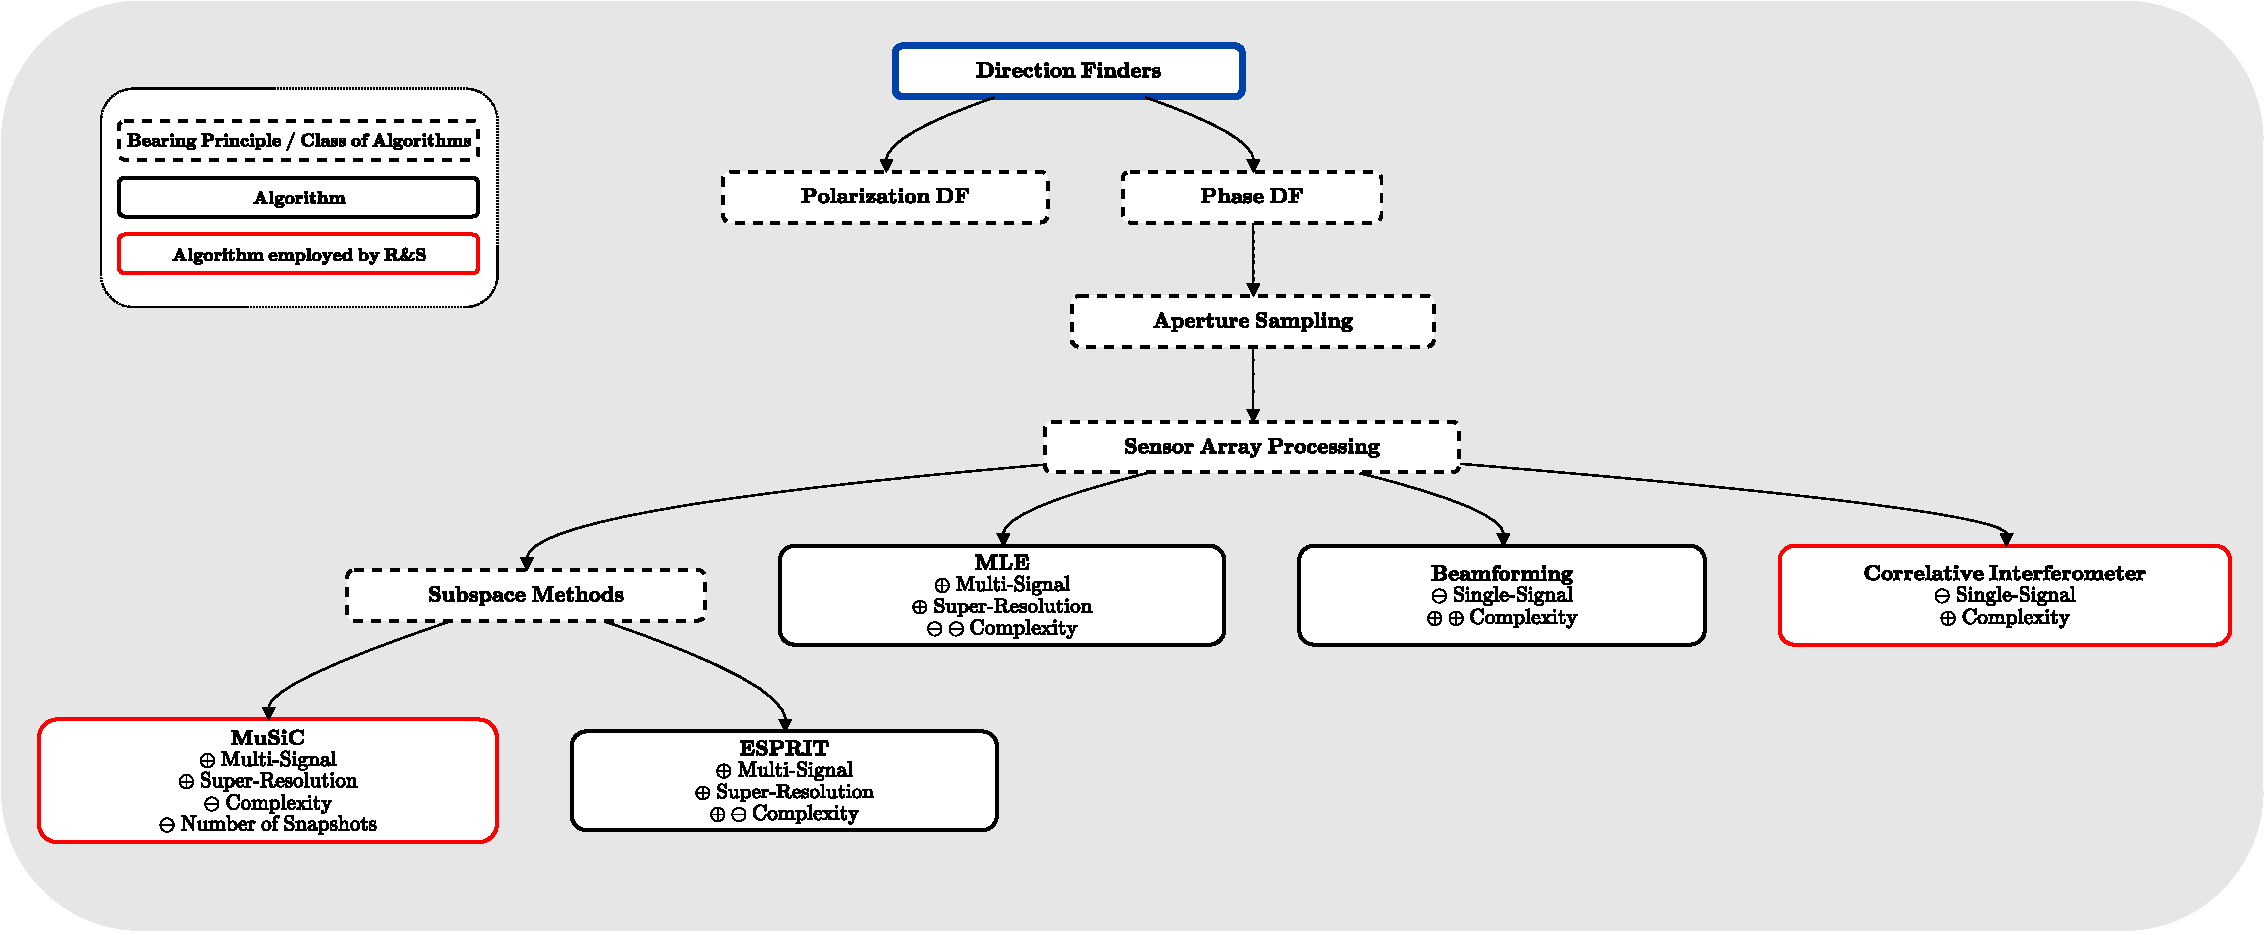
\includegraphics[width=1\textwidth]{figures/01_Introduction/direction_finder_graph.pdf}
    \caption{A graph representation of commonly employed direction finding techniques.}
    \label{fig:direction_finder_graph}
\end{figure}

\subsection{Challenges and Conventional Estimators}
In the domain of modern broadband direction finding, the accurate estimation of very short signals across extensive
bandwidths poses significant challenges. Conventional estimators, such as correlative interferometers and beamformers,
are computationally efficient and capable of providing accurate direction estimates after minimal measurements.
This efficiency renders them suitable for real-time applications and the estimation of short pulsed signals~%
\cite{meyer, tuncer.ch1, tuncer.ch2}.\\
However, these conventional methods inherently struggle with accommodating co-channel interference%
\footnote{The presence of multiple signals in the same frequency bin of the \gls{fft}.}
and multipath propagation. Additionally, they face limitations in resolving closely spaced signal sources when their
angular separation falls below the beam width of the antenna array. The performance of these methods is consequently
constrained in scenarios involving multiple incoming waves per frequency bin.\\

\subsection{Super-Resolution Methods} %TODO Subspace
To address the abovementioned limitations, super-resolution methods such as \gls{music} and \glsentryshort{esprit} are employed.
Grounded in subspace methods, these advanced techniques provide high-resolution \gls{doa} estimations and are
particularly effective in scenarios with multiple signals sharing the same frequency bin, as well as in situations where
signals have angular separations smaller than the antenna array's beamwidth. A more detailed exploration of the
\gls{music} method will be presented in \autoref{ch:OverviewMUSIC}.

Super-resolution methods are well-suited for continuous wave signals, requiring a sufficient number of
samples and a reasonable \gls{snr} to function effectively. They are capable of achieving angular resolutions as precise
as 0.1° and \glspl{rmse} of about 0.5°. However, these methods also demand higher computational resources and typically
need at least \( K \gtrsim 3M \) snapshots%
\footnote{One snapshot refers to a set of measurements that, while not necessarily captured simultaneously, are
collectively associated with a specific sampling cycle of an antenna array and includes samples from all antennas.
}
to produce reliable results, where \( M \) represents the number of antennas in
the \gls{uca}~\cite{tuncer.ch1}.


\section{Model Order Estimation}
The effectiveness of the aforementioned super-resolution methods relies on accurate estimates of the model order,
denoted as \( N \). This model order reflects the number of co-channel wavefronts concurrently impinging on the sensor array.\\
\gls{moe} is fundamentally grounded in the analysis of the eigenvalue profile of the signal's covariance matrix.
This analysis aims to distinguish signal eigenvalues from a cluster of low variance noise eigenvalues.
In an ideal scenario, the set of noise eigenvalues would have zero variance, facilitating a distinct separation between
signal and noise subspaces.\\
The classical \glspl{ic}, such as \gls{aic} and \gls{mdl}, which have been foundational in the field
for decades, will be elaborated in \autoref{sec:ClassicalInformationCriteria}.\\
The comprehensive discussion on the theoretical methodologies, including covariance matrix analysis, subspace concepts,
and the mathematical models underlying \gls{moe} and \gls{doa} estimation, will be detailed in \autoref{chap:DataModel}.


\subsection{Challenges in Conventional MOE}
While conventional \gls{moe} techniques, such as the \glspl{ic} \gls{aic} and \gls{mdl}, offer closed-form
solutions~\cite{barthelme2020}, making them relatively computationally efficient, they often falter under non-ideal
conditions:

\begin{itemize}
    \item \textbf{Low SNR:} In scenarios with low \glspl{snr}, these methods tend to underfit the model
    order, resulting in unreliable estimates~\cite{eft, yu22RCNN}.
    \item \textbf{High SIR:} With high \glspl{sir}, estimation errors increase without showing a distinct bias
    towards either overfitting or underfitting.
    \item \textbf{Sub-Sampled Covariance Matrix:} Utilizing sub-sampled covariance matrices decreases the goodness of fit
    of the estimated covariance matrix, leading to an increased variance in noise eigenvalues, a departure from theoretically
    expected noise eigenvalue distributions~\cite{meyer}, and the occurrence of negative eigenvalues~\cite{barthelme21sub, meyer}.
    \item \textbf{Limited Snapshots:} A limited number of signal snapshots%
\footnote{This tends to be the case when the number of snapshots \( K \) is of the same order as the number of antennas \( M \)~\cite{eft}}.
    affects the fidelity of the eigenvalue estimates~\cite{eft, barthelme2020, barthelme21sub}.
    \item \textbf{Coherent Multipath Interference:} Such interference typically results in overfitting, with the methods
    incorrectly interpreting multipath signals as separate, independent sources~\cite{yu22RCNN}.
    \item \textbf{Non-Gaussian Noise:} These estimators are designed to assume \gls{awgn}. Therefore, their performance
    is negatively impacted in the presence of non-Gaussian noise, especially in higher frequency ranges.
    \item \textbf{Susceptibility to Overfitting:} \gls{aic} and \gls{mdl} have been found to be generally prone to
    overfitting, especially when dealing with lower model orders~\cite{barthelme2020, eft}.
\end{itemize}

\subsection{Advancements in MOE}

\subsubsection*{Exponential Fitting Test (EFT)}
The \gls{eft} marks an algorithmic advancement in \gls{moe} for incoherent scenarios with a low number of snapshots and
the presence of non-Gaussian noise.
Introduced in~\cite{eft}, the \gls{eft} leverages the observation that noise eigenvalues approximately exhibit exponential
decay. It aims to detect mismatches greater than a threshold value between observed eigenvalues and the assumed exponential
profile, thereby effectively discerning signal from noise.
Despite subsequent enhancements to the \gls{eft} as detailed in~\cite{costa2007} and~\cite{costa2009}, the original

version still provides a baseline for comparative analysis against classical methods like \gls{aic} and \gls{mdl} and
the \glspl{dnn} explored in this thesis. A detailed elaboration on the \gls{eft} algorithm will be presented in \autoref{sec:eft}.

\subsubsection*{Recent Deep Learning Approaches}
The latest advancements in \gls{moe} have demonstrated the superiority of data-driven approaches, through the employment
of \glspl{dnn} over classical methods.
Research highlighted in~\cite{barthelme2020, barthelme21sub, yu22RCNN, yang2020, rogers2021} shows that \glspl{dnn}
outperform classical methods in terms of accuracy and computational efficiency, particularly in
challenging scenarios with sub-array sampling, multipath interference, and low numbers of snapshots.\\
These advanced \glspl{dnn} approaches represent a significant shift in \gls{moe}, providing more robust and adaptable
solutions in complex signal environments. A concise exploration of these DL-driven advancements in \gls{moe} will be
detailed in \autoref{sec:dl-advancements} before we will present our own \gls{dnn} approaches in \autoref{ch:model_exploration}
the choice for the input data and the underlying datasets in \autoref{ch:dataset_generation}.
The final chapters will than elaborate on the results and will also demonstrate the before mentioned caveats of the
classical approaches and we will end with a conclusion and outlook upon suggested future work in the field of \gls{moe}
in \autoref{ch:outlook}.

\endinput

% Recent advancements have demonstrated the superiority of data-driven approaches, particularly in the realm of
% \glspl{dnn}, for \gls{moe} \cite{barthelme2020, barthelme21sub, yu22RCNN, yang2020, rogers2021}. These DNN-based models have been shown to excel in MOE tasks,
% surpassing classical methods in accuracy and computational efficiency, especially in challenging scenarios with sub-array
% sampling. The study \cite{barthelme21sub} specifically highlights the effectiveness of NN-based estimation schemes in
% outperforming traditional estimators in both estimation accuracy and computational complexity.
% These innovative approaches represent a paradigm shift in MOE, offering more robust and adaptable solutions in complex
% signal environments.

% While many means towards improving the performance of these classical methods have been proposed, the latest research
% has shown the <überlegenheit> of fully data-driven approaches in the domain of \glspl{dnn}~\cite{barthelme2020, yu22RCNN}.
% - briefly mention the adaptations of classical methods:
% These limitations underscore the need for more robust and adaptable MOE methods, particularly in complex signal environments where traditional criteria may not provide accurate estimations.



% ---

% \cite{barthelme21sub}
% is the only paper that discusses DL-driven sulutions for \gls{doa} estimation and \gls{moe} in context of sub-array sampling.
% simulations show that the proposed NN-based estimation scheme iable to outperform the state-of-the-art estimators in terms of estimation accuracy and computational complexity

% \endinput
\chapter{Data Model}
\label{chap:DataModel}
This chapter outlines the data model that serves as the foundation for the direction-finding algorithms and various
\gls{moe}-methods explored in this thesis. The data model encompasses the signal model, the antenna model, and the
measurement model, which we will introduce in the following sections. The content of this chapter is based on the
master's thesis by~\cite{meyer} and follows common conventions in the field of \gls{doa} estimation as outlined in~\cite{}

%---------------------------------------------------------------------------


\imgsection{Emitter Model}{figures/02_SignalModel/emitter_left.pdf}
\label{sec:EmitterModel}

The emitter model captures both the wave characteristics and the spatial relationship of the received field to the
antenna array. Following the guidelines by~\cite[ch2.2]{meyer}, we assume identical polarization—either vertical or
horizontal—for the incoming wave and all \( M \) antennas.

The Poynting vector \( \bfm{S} \) indicates the directional electromagnetic energy flux of the received field and is
orthogonal to its components. This fundamental relationship can be expressed mathematically as
\( \bfm{S} = \bfm{E} \times \bfm{B} \), where \( \bfm{E} \) and \( \bfm{B} \)
are the electric and magnetic field strengths, respectively~\cite[ch2.1]{demmel}.
\\
Derived from the Poynting vector, the \gls{doa} vector \( \bfT \) can be interpreted as the
directional components of \( \bfm{S} \). It is defined as in Equation~\eqref{eq:DOAVector}.
\begin{equation}
    \bfT  =
    \begin{bmatrix}
        \azim \\
        \elev
    \end{bmatrix}, \azim\;\in \{\azim\;\in \mathbb{R} \quad|\quad 0 \le \azim < 360^\circ\},
    \elev \in \{\elev \in \mathbb{R} \quad|\quad -90^\circ \le \elev \le 90^\circ  \}.
    \label{eq:DOAVector}
\end{equation}

The two angles \( \azim \) and \( \elev \) represent the azimuth and elevation angles, and can be
interpreted visually via the beautiful illustration by~\cite{meyer} in \autoref{fig:PointingVector}.

\begin{figure}[H]
    \centering
    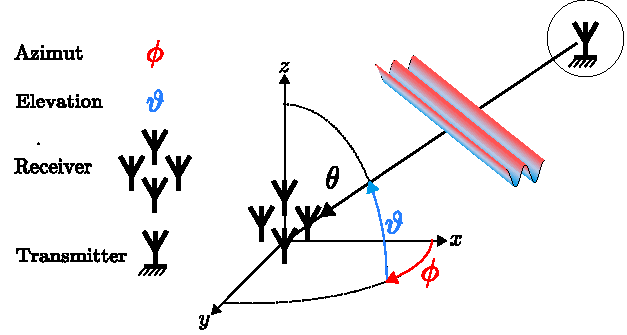
\includegraphics[width=0.6\textwidth]{figures/02_SignalModel/pointing_vect.drawio.pdf}
    \caption{Impinging wave-front - a visual representation of the Poynting vector \( \bfT \)}
    \label{fig:PointingVector}
\end{figure}
The x-axis of the cartesian coordinate system in \autoref{fig:PointingVector} is pointing towards the north, the
y-axis towards the east. Another simplifying assumption is the stationarity of the emitter during the duration of
one sampling period, which implies \( \frac{d\bfT}{dt} = 0 \).
\\

The emitter signal \( \widetilde{s}(t) \) can be expressed as a complex baseband signal \( s(t) \) modulated by a
carrier frequency \( f_C \)~\cite{tuncer.ch1}:
\begin{equation}
    \widetilde{s}(t) = s(t) \cdot \exp(j 2\pi f_C t)
    \label{eq:EmitterSignal}
\end{equation}
%---------------------------------------------------------------------------


\imgsection{Antenna Model}{figures/02_SignalModel/antenna.pdf}
\label{sec:AntennaModel}
The antenna model considers the directivity \( c(\theta, f_C) \) of real antennas which may distort the phase and
amplitude of received signals based on their frequency \( f_C \) and the angle of incidence \( \theta \).
The model assumes that the antenna is passive and does not amplify the received signal.
The voltage at the base of the antenna for an incoming wave is described in Equation~\eqref{eq:AntennaVoltage}.

\begin{equation}
    \widetilde{s}_A(t) = c(\theta, f_C) \cdot s(t) \cdot \exp(j 2\pi f_C t), \quad c \in \{c \in \mathbb{C} \,|\, |c| \leq 1\}
    \label{eq:AntennaVoltage}
\end{equation}
%---------------------------------------------------------------------------

\section{Measurement Model}
\label{sec:MeasurementModel}

\subsection{Introduction}
This section aims to elaborate on the measurement model used in the context of a \glsdesc{uca}.
A UCA comprises \( M \) antennas, uniformly distributed along a circle. The array enables the formation of an \( M \)-dimensional measurement
vector.
This measurement vector serves as the crucial link between the physical characteristics of incoming waves and the
digital signals that are subsequently processed.
The section further elaborates on how this model accommodates both single and multiple incoming waves.


\subsection{Single-Wave Case}
For a single incoming wave, each antenna \( A_m \) in an array of \( M \) antennas observes a phase \( \varphi_m \).
The phase differences \( \Delta\varphi_m \) between a reference antenna \( A_1 \) and all other antennas
\( A_m, \forall m \in \{2, 3, \ldots, M\} \) are expressed as:
\begin{align}
    \Delta\varphi_m(t) & = \varphi_m(t) - \varphi_1(t)                                                                                  \\
                       & = \pi \underbrace{\frac{d_{\text{Ant}}}{\lambda_C}}_D \cos(\elev) \sin\left(2\pi\frac{m-1}{M}-\azim\right).
    \label{eq:PhaseDiff}
\end{align}
The term \( \frac{d_{\text{Ant}}}{\lambda_C} \) is commonly denoted as aperture \( D \) and its influence on the array's
performance is discussed in Appendix~\ref{app:sec:ApertureInfluence}.\\
The narrowband approximation is a crucial assumption in~\eqref{eq:PhaseDiff}. It is expressed as
\( f_B \ll f_C \rightarrow d_{\text{Ant}}/\lambda_C \gg d_{\text{Ant}}/\lambda_B \), where \( f_B \) is the highest
occurring frequency in the baseband and \( f_C \) is the carrier frequency. This inequality implies that the phase
differences in the baseband signal are negligibly small compared to those at the carrier frequency.~\cite{tuncer.ch3}.

The relationship between the phase differences \( \Delta\varphi_m \) and the \gls{uca} are illustrated in \autoref{fig:UCA}.
\begin{figure}[H]
    \centering
    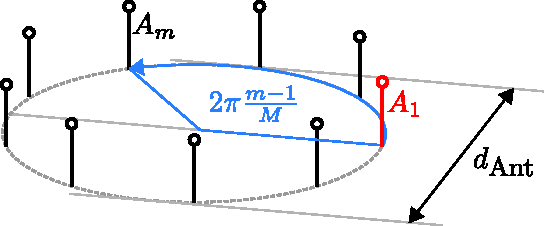
\includegraphics[width=0.5\textwidth]{figures/02_SignalModel/uca.pdf}
    \caption{The effect of the \gls{uca} on the phase differences \( \Delta\varphi_m \)~\cite{meyer}}.
    \label{fig:UCA}
\end{figure}

This leads to the antenna terminal voltage for the \( m \)-th antenna relative to the reference antenna as:
\begin{equation}
    \widetilde{s}_{A_m}(t) = c(\theta,f_C) \cdot \exp(j\Delta\varphi_m) \cdot \widetilde{s}(t)                \\
\end{equation}

The antenna terminal voltages are sampled and transformed into the complex baseband, introducing measurement noise. % TODO: Transformed to baseband. True?
This noise is assumed to be complex \gls{awgn} with zero mean and variance \( \sigma_\eta^2 \).
\( \eta_m \sim \mathcal{C}\mathcal{N}(0,\sigma_\eta^2) \), \( \eta_m \in \mathbb{C} \), and is statistically independent of the
baseband signal. The index \( k \) is defined as \( k = t / T_s \), where \( T_s \) is the sampling period.
This results in the measured voltage \( x_m[k] \) for the \( m \)-th antenna:
\begin{equation}
    x_m[k] = \underbrace{c(\bfT,\lambda_C) \cdot \exp(j\Delta\varphi_m)}_{a_m(\bfT)} \cdot s[k] + \eta_m[k]
    \label{eq:MeasScalar}
\end{equation}

The term \( a_m(\bfT) \) in~\eqref{eq:MeasScalar} is the \( m \)-th component of the steering vector \( \bfm{a}(\bfT) \),
which represents the array's spatial response to an impinging signal with from \( \bfT \), including amplitude
and phase information~\cite{oap.ch9}.
\begin{equation}
    \bfm{a}(\bfT) =
    \begin{bmatrix} a_1(\bfT) & a_2(\bfT) & \cdots & a_M(\bfT) \end{bmatrix}^T \in \mathbb{C}^{M}
    \label{eq:SteeringVector}
\end{equation}

Expanding~\eqref{eq:MeasScalar} to all \( M \) antennas yields the measurement vector \( \bfm{x}[k] \in \mathbb{C}^{M} \):
\begin{equation}
    \bfm{x}[k] = \bfm{a}(\bfT) \cdot s[k] + \bfm{\eta}[k],\quad \text{where}\: \bfm{\eta}[k] \sim \mathcal{C}\mathcal{N}(0,\sigma_\eta^2 \bfm{I}_M)
    \label{eq:MeasVecSingle}
\end{equation}

Considering the collection of all \( K \) measurements, results in the \textit{measurement matrix} \( \bfm{X} \)
\begin{equation}
    \bfm{X} = \begin{bmatrix} \bfm{x}[1] & \bfm{x}[2] & \cdots & \bfm{x}[K] \end{bmatrix} \in \mathbb{C}^{M \times K}
    \label{eq:MeasMatSingle}
\end{equation}
The measurement matrix \( \bfm{X} \) is commonly denoted as \( \bfm{x} \) -- measurement vector without the discrete time index.

The array manifold \( \mathfrak{A} \) is a function \( \mathfrak{A} : \mathbb{R}^2 \to \mathbb{C}^{M} \) that transforms
unit amplitude signals from spatial directions \( \bfT \in \mathbb{R}^2 \) into steering vectors
\( \bfm{a}(\bfT) \in \mathbb{C}^{M} \)~\cite{oap.ch4, tuncer.ch1}. Essentially, it characterizes the array's spatial
response to an incoming unit amplitude signal for given spatial parameters \( \bfT \)~\cite{yu22RCNN}.

\begin{figure}[H]
    \centering
    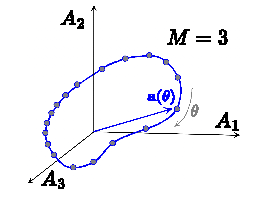
\includegraphics[width=0.6\textwidth]{figures/02_SignalModel/array_manifold.pdf}
    \caption{The array manifold \( \mathfrak{A} \)~\cite[ch4.5.2]{demmel}}
    \label{fig:ArrayManifold}
\end{figure}

\autoref{fig:ArrayManifold} visually represents the array manifold \( \mathfrak{A} \) by displaying the locus of
steering vectors for an antenna array with \( M = 3 \) antennas.
\\

\subsubsection*{Multi-Wave Scenario}
In scenarios involving multiple incoming waves, let \( \Theta = \{\bfT_1, \ldots, \bfT_N\} \) represent the set of
directions of theses \( N \)%
\footnote{The number of impinging waves \( N \) is also referred to as the \textbf{model order}.}
impinging waves. The Steering Matrix \( \bfm{A} \) is then defined as the set of steering vectors
corresponding to this \( \Theta \). The matrix has dimensions \( M \times N \) and is expressed as:
\begin{align}
    \bfm{A}(\bfm{\Theta}) =
    \begin{bmatrix} \bfm{a}(\bfT_1) & \cdots & \bfm{a}(\bfT_N) \end{bmatrix}
    \label{eq:SteeringMatrix}
\end{align}
Hence, the measurement vector in this multi-wave scenario becomes:
\begin{align}
    \bfm{x}[k] = \bfm{A}(\bfm{\Theta}) \bfm{s}[k] + \bfm{\eta}[k].
    \label{eq:MeasVecMult}
\end{align}

% \subsubsection*{Discrete Approximation of the Array Manifold}

% Immediately following our discussion on the continuous array manifold \( \mathfrak{A} \), it is pertinent to introduce
% its discrete approximation \( \widehat{\mathfrak{A}} \). This approximation is constructed from a finite set
% \( \{\bfT_1', \ldots, \bfT_Q'\} \) of spatial directions and serves as a sampled representation of \( \mathfrak{A} \).
% It is defined as:
% \begin{align}
%     \widehat{\mathfrak{A}} =
%     \begin{bmatrix}
%         a_1(\bfT_1') & \cdots & a_1(\bfT_Q') \\
%         \vdots       & \ddots & \vdots       \\
%         a_M(\bfT_1') & \cdots & a_M(\bfT_Q')
%     \end{bmatrix},
%     \quad \widehat{\mathfrak{A}} \in \mathbb{C}^{M \times Q}.
% \end{align}
% This discrete approximation will be essential for subsequent computational applications, such as the \gls{music} algorithm.




\section{Covariance Matrix and Subspaces}
\label{sec:CovarianceMatrix}
In the realm of advanced signal processing, covariance matrices serve as a cornerstone, particularly for
super-resolution \gls{doa} techniques such as \gls{music}, detailed in~\autoref{ch:OverviewMUSIC}. These techniques rely
on the evaluation of the subspaces spanned by the eigenvectors derived from the covariance matrix.
On the other hand, \gls{moe} methods, discussed in~\autoref{ch:ModelOrderEstimation}, as well as the Deep Learning (DL) approaches
examined in this thesis, focus primarily on the eigenvalues of the covariance matrix. This section delves into the
mathematical foundations of the covariance matrix, elucidates its significance in the derivation of signal and noise
subspaces, and outlines the conditions required for its accurate estimation in real-world applications.


\subsection{Subspaces}
\label{sec:sub:subspaces}
The notion of signal and noise subspaces is pivotal in the field of \gls{doa} estimation, especially when employing
super-resolution algorithms such as \gls{music}, as elaborated in~\autoref{ch:OverviewMUSIC}.
In mathematical terms, the signal subspace represents the span of measurement vectors \( \bfm{x}_i[k] \) in complex
space \( \mathbb{C}^M \) for a given \( \bfT_i \). This span can also be understood as a subset of points in
\( \mathbb{C}^M \) reachable by the linear combinations of the measurement vectors. Thus, the signal subspace
\( \bfm{U}_S \) is formally defined as:
\begin{equation}
    \bfm{U}_S = \mathrm{span}\{\bfm{x}_i[k]\} \subseteq \mathbb{C}^M
\end{equation}
The concept of the signal subspace provides an intuitive geometric representation of the measurement vectors as
previously described in~\autoref{sec:MeasurementModel}, given \( M = 3 \) antennas in three-dimensional space.
For a single-wave scenario, the noiseless measurement vector, \( \bfm{x}_i[k] \), manifests as a finite line
passing through the origin in \( \mathbb{C}^M \), characterized by its direction vector \( \bfm{a}(\bfT) \)~\cite{meyer}.
In a multi-wave context, each measurement vector \( \bfm{x}_i[k] \) can be considered a linear combination of
vectors \( \bfm{a}(\bfT_n) \). These vectors span the signal subspace \( \bfm{U}_S \), which is mathematically
defined as \( \bfm{x}_i[k] \in \bfm{U}_S \subseteq \mathbb{C}^M \)~\cite{meyer}. Both abovementioned scenarios
are illustrated in~\autoref{fig:subspace}.

\begin{figure}[H]
    \centering
    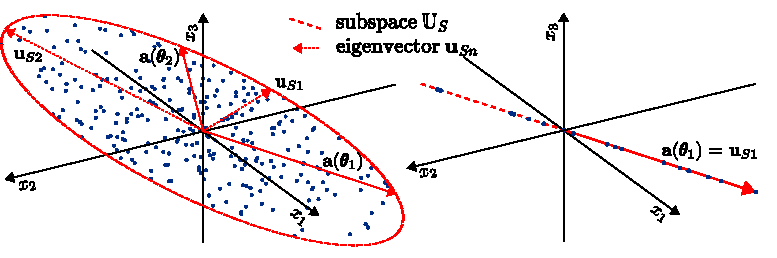
\includegraphics[width=0.9\textwidth]{figures/02_SignalModel/subspace.pdf}
    \caption{The signal subspace \( \bfm{U}_S \) for two and a single impinging wave(s)~\cite{meyer}}
    \label{fig:subspace}
\end{figure}

As per \autoref{eq:MeasVec}, additive white Gaussian noise \( \bfm{\eta}[k] \sim \mathcal{C}\mathcal{N}(0,\sigma_\eta^2\bfm{I}) \)
superimposes the linear combinations of steering vectors \( \bfm{a}(\bfT_n) \).
Given the presence of \( N \) waves, which span an \( N \)-dimensional signal subspace \( \bfm{U}_S \),
the noise subspace \( \bfm{U}_\eta \) spans an \( M \)-dimensional sphere in \( \mathbb{C}^M \).

Both subspaces are characterized by their eigenvectors \( \bfm{U} \) and eigenvalues \( \bfL \).
\begin{align}
    \bfm{C} & = \sum_{m=1}^M \lambda_m \bfm{u}_m \bfm{u}_m^H                                                 \\
            & = \bfm{U}_S \bfm{\Lambda}_S \bfm{U}_S^H + \bfm{U}_{\eta} \bfm{\Lambda}_{\eta} \bfm{U}_{\eta}^H
    \label{eq:EigenvalueDecomposition1}
\end{align}
In \autoref{eq:EigenvalueDecomposition1}, the eigenvalues
\( \bfm{\Lambda} = \text{diag}\{\lambda_1, \lambda_2, \ldots, \lambda_N\} \) and their corresponding eigenvectors
\( \bfm{U} = [\bfm{u}_{1},\ldots,\bfm{u}_{N}] \) are sorted in descending order, that is,
\( \lambda_1 \geq \lambda_2 \geq \cdots \geq \lambda_N \), as described in~\cite{tuncer.ch5}.

The signal subspace \( \bfm{U}_S \) is spanned by the first \( N \) eigenvectors,
\( \bfm{U}_S = [\bfm{u}_{1},\ldots,\bfm{u}_{N}] \), corresponding to the largest \( N \) eigenvalues.
Conversely, the noise subspace \( \bfm{U}_{\eta} \) is spanned by the remaining eigenvectors
\( \bfm{U}_{\eta} = [\bfm{u}_{N+1}, \ldots, \bfm{u}_{M}] \), which correspond to the smaller eigenvalues.

% \begin{equation*}
%     \bfm{U} &= \begin{bmatrix} \bfm{u}_{1} & \cdots & \bfm{u}_{N} & \bfm{u}_{N+1} & \cdots & \bfm{u}_{M} \end{bmatrix}
% \end{equation*}

\subsection{Covariance Matrix and its Eigenvalue Decomposition}
Expanding on the foundational principles of signal and noise subspaces, the covariance matrix \( \bfm{C} \) plays an
indispensable role in eigenvalue-based methods for \gls{doa} and \gls{moe} estimation. The covariance matrix captures
the second-order statistics of the received signals\footnote{Refer to \autoref{app:sec:GeneralCovMatrix} for a
    comprehensive form of the covariance matrix}, thereby integrating both their signal and noise attributes.

The covariance matrix \( \bfm{C} \) was previously introduced in \autoref{eq:EigenvalueDecomposition1}, constructed
from the eigenvalues \( \bfm{\Lambda} \) and eigenvectors \( \bfm{U} \) that characterize the signal and noise
subspaces. Given that these characteristics are not known a priori and are essentially the information sought for
\gls{doa} and \gls{moe} estimation, alternative methods must be employed for constructing the covariance matrix to
then being able to perform an eigenvalue decomposition.

If the signal and noise vectors are zero mean, and if the noise is spatially white and statistically independent of the
source signals~\cite{tuncer.ch5}, then the \( M \times M \) array covariance matrix can be calculated as:
\begin{align}
    \bfm{C}_x & = \mathbb{E}[\bfm{x}[k] \bfm{x}^H[k]]  \label{eq:CovarianceExpanded1}                                                                                                                                                                   \\
              & = \bfm{A} \mathbb{E}[\bfm{s}[k] \bfm{s}^H[k]] \bfm{A}^H + \bfm{A} \mathbb{E}[\bfm{s}[k] \bfm{\eta}^H[k]] + \mathbb{E}[\bfm{\eta}[k] \bfm{s}^H[k]] \bfm{A}^H + \mathbb{E}[\bfm{\eta}[k] \bfm{\eta}^H[k]]  \label{eq:CovarianceExpanded2} \\
              & = \underbrace{\bfm{A} \mathbb{E}[\bfm{s}[k] \bfm{s}^H[k]] \bfm{A}^H}_{\bfm{C}_S} + \; {\color{red}{0}} \; + \underbrace{\sigma_\eta^2 \bfm{I}}_{\bfm{C}_\eta} \label{eq:CovarianceExpanded3}                                                 \\
              & = \bfm{C}_S + \sigma_\eta^2 \bfm{I}  \label{eq:CovarianceExpanded4}
\end{align}\cite[Chapter 4]{meyer}

As shown in~\eqref{eq:CovarianceExpanded2}, the measurement vector \( \bfm{x} \) is decomposed into its signal component
\( \bfm{s} \), transformed by the steering matrix \( \bfm{A}(\bfm{\Theta}) \), and additive noise \( \bfm{\eta} \),
based on \autoref{eq:MeasVecMult}.
The terms related to cross-correlation in~\eqref{eq:CovarianceExpanded2} become zero, given the assumption that the
signal and noise are zero-mean and uncorrelated. This simplification leads to the final form of the covariance matrix
as shown in~\eqref{eq:CovarianceExpanded4}.
The noise covariance matrix \( \bfm{C}_\eta \) is denoted as \(\sigma_\eta^2 \bfm{I}\), where \(\sigma_\eta^2\) is the noise variance. Similarly,
\( \bfm{C}_S \) represents the signal covariance matrix.


\subsubsection*{Estimation of the Covariance Matrix}
In real-world scenarios, the covariance matrix \( \bfm{C}_x \) is typically estimated from a finite set of snapshots
\( K \) of the measurement vector \( \bfm{x}[k] \). The maximum-likelihood estimate for \( \bfm{C}_x \) is given by:
\begin{equation}
    \C = \frac{1}{K} \sum_{k=1}^{K} \bfm{x}[k] \bfm{x}^H[k]
    \label{eq:SampledCovarianceMatrix}
\end{equation}
The fidelity of the covariance matrix approximation improves as the number of snapshots \( K \) increases,
asymptotically approaching the true covariance matrix as \( K \to \infty \)~\cite{tuncer.ch7}.\\
All quantities derived from the estimated covariance matrix are denoted as follows%
\footnote{The model order \( N \), through its own merit, has earned the privilege of wearing a hat when estimated.}
\begin{align*}
    \bfm{U} & \mapsto \widehat{\bfm{U}} \\
    \bfm{U}_S & \mapsto \UsH \\
    \bfm{U}_{\eta} & \mapsto \UnH \\
    \bfL & \mapsto \widehat{\bfL} \\
\end{align*}


It is essential to have more samples \( K \) than antennas \( M \) for a reliable covariance matrix approximation.
This requirement ensures that each distinct eigenvalue of the true covariance matrix corresponds to a unique cluster in
the eigenvalue distribution. A sufficient number of samples allows for the separation of these clusters, enabling
accurate estimation of eigenvalues and eigenvectors, and thereby reducing ambiguity and enhancing the approximation's
accuracy~\cite{tuncer.ch7}.



\subsubsection*{Eigenvalue Decomposition of the Covariance Matrix}
The covariance matrix \( \bfm{C}_x \) is a Gram matrix and is positive semi-definite, a trait ensuring that its
eigenvalues are real and non-negative~\cite{tuncer.ch4}.

\begin{align}
    \bfL & = \sigma_\eta^2 + \bfL_S                                                                                                  \\
                  & = \begin{bmatrix} \lambda_{S_1} + \sigma_\eta^2 & \cdots & \lambda_{S_N} + \sigma_\eta^2 & \sigma_\eta^2 & \cdots & \sigma_\eta^2 \end{bmatrix}^T
    \label{eq:eigval_superimposed}
\end{align}\cite{oap.ch5, meyer}

All eigenvalues are superimposed by the noise variance \( \sigma_\eta^2 \), causing the covariance matrix to become positive
finite~\cite{tuncer.ch4, oap.ch5}. \\
Each noise eigenvalue \( \lambda_i \in \bfL_{\eta}\) for \( i \in \{N, \ldots, M\} \) is normally distributed \( \lambda_i \sim \mathcal{N}(\sigma^2_{\eta}, 0) \)
with mean \( \sigma^2_{\eta} \) and variance 0.

When \( \widehat{\bfL} \) is considered for a finite number of snapshots, the
noise eigenvalues \( \lambda_i \in \bfL_{\eta}\) for \( i \in \{N, \ldots, M\} \) empirically appear to be drawn from independent normal distributions
whose means are less than \( \sigma^2_{\eta} \) and separated approximately uniformly.
These distributions converge asymptotically to the theoretical value as \( K \to \infty \).
\begin{equation}
    \mathcal{N}(\mathbb{E}[\lambda_{i, \eta}], \sigma^2_{\lambda_{i, \eta}}) \stackrel{K \rightarrow \infty}{\xrightarrow{\hspace*{1cm}}} \mathcal{N}(\sigma^2_{\eta}, 0), \quad i \in \{N, \ldots, M\}
\end{equation}

\section{Incoherent Measurement Model}
\label{sec:InherentMeasurementModel}

The incoherent measurement model represents an adaptation of the coherent measurement framework, previously established,
to situations where the number of available antenna paths \( L \) is fewer than the total number of antennas \( M \).
This adaptation is necessitated by resource constraints inherent to each antenna path%
\footnote{Tuners, analog filters, ADCs, DDCs, ...\cite{demmel}.},
that limit the number of paths that can be simultaneously processed.
Considering a scenario with 9 antennas and 3 antenna paths, one path is permanently allocated to the reference antenna,
while the other two are switched in time-division across the remaining antennas.

\subsection{Incoherent Measurement Vector}
\label{subsec:IncoherentMeasurementVector}
The incoherent measurement vector \( \bfm{x}'[k] \) is an extension of the coherent measurement vector introduced
in \autoref{eq:MeasVec} for cases when \( L < M \). It captures the signal from a subset of antennas at each snapshot
and is formulated as follows~\cite[Chapter 6]{meyer}:
\begin{align}
    \bfm{x}'[k] &= \bfm{D}[j] \bfm{x}[k], & \bfm{x}' \in \mathbb{C}^{M} \\
    j &= \text{mod}(k-1, J) + 1.
\end{align}
Here, \( k \) represents the snapshot index, and \( j \) indicates the specific switching step within a cycle determined
by the total number of steps \( J \) -- \( J \) being the number of subarrays. This model assumes a time-division strategy, where different subsets of antennas
are activated at different times to form the overall measurement.%

\begin{table}[H]
    \caption{Sampling cycle for a \gls{uca} with \( M = 9 \) antennas and \( L = 3 \) RF-paths.}
    \label{tab:SamplingCycle}
    \centering
    \begin{tabular}{>{\bfseries}c*{5}{c}}
      \toprule
      Antenna Base & Path 1-2 & Path 1-3 & Path 2-3 & Diagonal & DF1 DF2 DF3 \\
      \midrule
      1 & \(x_{12}\) & \(x_{19}\) & \(x_{29}\) & \(\varnothing\) & \(A_{1}\, A_{2}\, A_{9}\) \\
      2 & \(x_{13}\) & \(x_{18}\) & \(x_{38}\) & \(\varnothing\) & \(A_{1}\, A_{3}\, A_{8}\) \\
      3 & \(x_{14}\) & \(x_{17}\) & \(x_{47}\) & \(\varnothing\) & \(A_{1}\, A_{4}\, A_{7}\) \\
      4 & \(x_{15}\) & \(x_{16}\) & \(x_{56}\) & \(x_{11}\) & \(A_{1}\, A_{5}\, A_{6}\)  \\
      \vdots & \vdots & \vdots & \vdots & \vdots & \vdots \\
      12 & \(x_{78}\) & \(x_{79}\) & \(x_{89}\) & \(x_{88}\) & \(A_{7}\, A_{8}\, A_{9}\) \\
      \bottomrule
    \end{tabular}
  \end{table}


\subsection{Impact on the Estimated Covariance Matrix}
\label{subsec:ImpactOnTheCovarianceMatrix}
Subsampling in an incoherent measurement setup negatively affects the estimation of the covariance matrix, \( \Csub \), as it's
based on a subset of the full antenna array signals at each snapshot. This leads to a covariance matrix that may not
fully capture the true signal correlations, denoted as:
\begin{equation}
    \Csub = \frac{1}{KJ}\sum_{\substack{k=1 \\ j=\text{mod}(k-1, J) + 1}}^{KJ} \text{selDiag} \left(\bfm{D}[j] \bfm{x}[k] \bfm{x}^H[k] \bfm{D}^H[j] \right)
    \label{eq:sub_sampled_covmat}
\end{equation}

The function ``selDiag'' selects the diagonal elements of the sub-array covariance matrices according to the switching
scheme outlined in \autoref{tab:SamplingCycle}. This process is essential to ensure that the diagonal elements of the
covariance matrices are sampled only once per antenna cycle. While the discarding of most off-diagonal elements certainly
results in a loss of information, the employment of according scaling factors to compensate for the varied accumulation
frequencies of the principal and off-diagonal elements has been shown to result in numerical errors.
As a result of the degraded estimation of the covariance matrix, the eigenvalues derived from \( \Csub \) exhibit
increased variance and potentially negative values.
The situation is further exacerbated when the number of snapshots is low, as more samples are generally required to achieve
an accurate estimation of the true covariance matrix.
This corruption of the eigenvalues leads to various challenges with typically employed \gls{doa} estimation techniques,
and exacerbates the problem of model order selection~\cite[Chapter 6, 8]{meyer}.

While the incoherent measurement vector and the respective sub-sampled covariance matrix will be the basis for all following sections, we will no longer distinguish
between coherent and incoherent values or symbols throughout the rest of this thesis for sake of convenience.


\section{Conclusion}
\label{sec:Conclusion}

\begin{figure}[H]
    \centering
    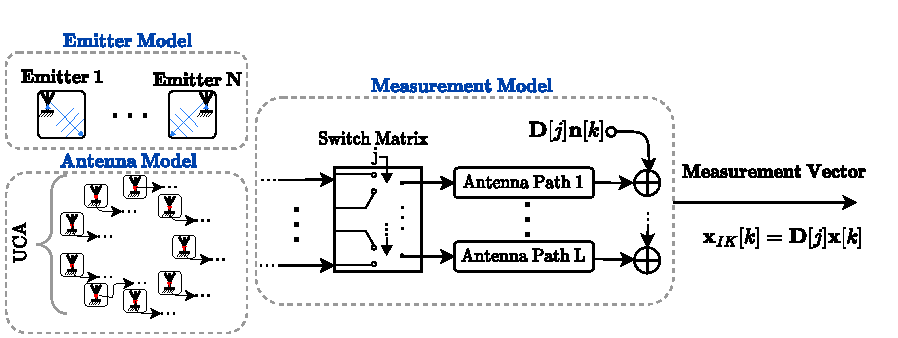
\includegraphics[width=1\textwidth]{figures/02_SignalModel/meas_model.pdf}
    \caption{The incoherent measurement model}
    \label{fig:IncoherentMeasurementModel}
\end{figure}

The data model as illustrated in \autoref{fig:IncoherentMeasurementModel} showcases the interplay of the various
``sub-models'' explored in this chapter. Starting with the emitter model, which assumed the far-field propagation of
a narrowband signal, followed by the antenna model, which considered the directivity of real antennas, and finally
the measurement model (\autoref{sec:MeasurementModel}), which captured the spatial relationship of the received
fields to the antenna array. The measurement model depicted in \autoref{fig:IncoherentMeasurementModel}, shows the
extension of the coherent measurement model, which was explored in the previous section.


\endinput





\chapter{DoA Estimation: Super-resolution via MuSiC}
\label{ch:OverviewMUSIC}

\section{Introduction}
The \gls{music} algorithm is a prominent high-resolution method in the realm of \gls{doa} estimation.
This chapter offers a brief overview of its fundamental mathematical underpinnings and practical considerations,
particularly highlighting the essentiality of prior knowledge of the model order \( N \). Although, a manifold of
variations of \gls{music} exist, this chapter focuses exclusively on the original \gls{music} algorithm, since these
variations still require \( N \) to be known a priori.

As hinted in the introductory chapter, super-resolution methods, including \gls{music}, differ significantly from
conventional \gls{doa} estimation methods. It was previously mentioned that conventional techniques like correlation
interferometers and beam-formers, while computationally efficient, fail to handle multiple incoming waves within a single
frequency bin. Super-resolution methods, on the other hand, are capable of estimating the \gls{doa} of signals even when
their angular separation is less than the beam-width of the antenna array. This capability is often refferred to as
``super-resolution''~\cite{tuncer.ch1}.

Theoretically, \gls{doa} estimation could be optimally achieved using a \glsdesc{mle} approach, as outlined
in~\cite{tuncer.ch1}. However, this method becomes computationally unsustainable for large antenna arrays, as it requires
an exhaustive search over an \( N \)-dimensional complex space.
In contrast, while the computational complexity of \gls{music} is higher compared to conventional methods, it remains
feasible for large arrays by reducing the search to a two-dimensional grid.
However, a notable limitation of \gls{music} is its requirement for a
higher number of snapshots \( K \), whereas conventional methods can already achieve reasonable results with a single
snapshot. This requirement for a higher number of snapshots is due to the need for a higher
\gls{snr} for accurate estimation~\cite{tuncer.ch1}.

\section{The MuSiC Algorithm}
\label{sec:music_algorithm}
The \gls{music} algorithm is predicated on the principles of subspace decomposition which were outlined in~\autoref{sec:CovarianceMatrix}.
It exploits the orthogonality between the signal subspace \( \UsH \) and the noise subspace \( \UnH \).
This perpendicularity is mathematically captured by the vanishing inner product between these two subspaces, as indicated
in~\autoref{eq:orthogonality}.

\begin{equation}
    \UsH^H \UnH = 0
    \label{eq:orthogonality}
\end{equation}

Building upon the concept that \( \UsH \) comprises a linear combination of the steering vectors \( (\bfm{a}(\bfT_1), \ldots, \bfm{a}(\bfT_N)) \),
as discussed in~\autoref{sec:sub:subspaces}, this orthogonality condition can be reformulated such that it becomes a
function of \( \bfT \).

\begin{equation}
    \bfm{a}^H(\bfT) \UnH = 0 \quad \text{for } \bfT \in \{\bfT_1, \ldots, \bfT_N\}
    \label{eq:orthogonality2}
\end{equation}

\autoref{eq:orthogonality2} underpins the formulation of the MuSiC pseudo-spectrum \( \widehat{P}_{\text{MuSiC}}(\bfT) \), defined as:
\begin{equation}
    \widehat{P}_{\text{MuSiC}}(\bfT) = \frac{1}{\|\bfm{a}^H(\bfT) \UnH \|^2}
\end{equation}

The MuSiC pseudospectrum is instrumental in identifying the \gls{doa} of incoming signals, as it exhibits local maxima
corresponding to the true \gls{doa} angles. In an ideal scenario without noise, the pseudo-spectrum would exhibit
infinite peaks at these angles. With the prerequisite knowledge of the model order \( N \), which signifies the number
of impinging waves, the task of estimating the \glspl{doa} translates into an optimization problem. The objective is to
locate the \( N \) angles \( \bfT \) that maximize the pseudo-spectrum. This optimization problem can be formally stated as:

\begin{equation}
    \{\widehat{\bfT}_1, \ldots, \widehat{\bfT}_N\} = \argmax_{\bfT} \widehat{P}_{\text{MuSiC}}(\bfT)
\end{equation}

\subsubsection*{Visualizing the MuSiC Pseudospectrum}
\autoref{fig:music_pseudospectrum} presents a three-dimensional conceptual plot of the pseudo-spectrum, delineated across
azimuth \( \azim \) and elevation \( \elev \) angles. The pronounced peaks, marked in red, correspond to the estimated
\glspl{doa} of the impinging signals. Notably, \( \bfT_3 \) and \( \bfT_4 \) display discernible deviations from the true
local maxima within the spectrum. Errors in the \gls{doa} estimates are usually quantified via the \gls{rmse} metric,
expressed in degrees.

\begin{figure}[H]
    \centering
    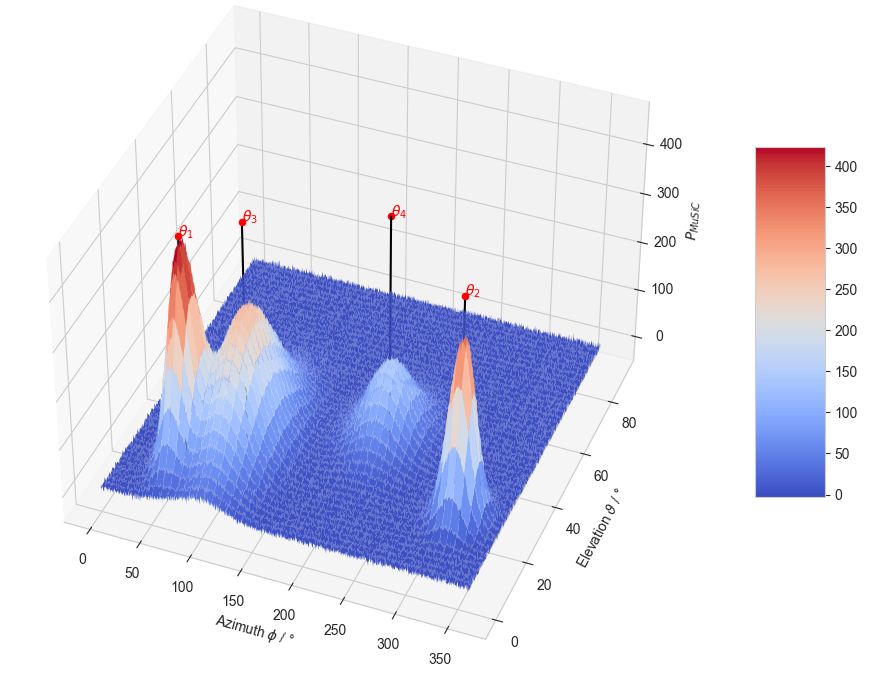
\includegraphics[width=0.76\textwidth]{figures/03_music/music_spectrum.png}
    \caption{Conceptual visualization of the MuSiC pseudo-spectrum for \( N = 4 \) impinging waves.}
    \label{fig:music_pseudospectrum}
\end{figure}

In practice, the accuracy of the peak detection directly influences the reliability of the \gls{doa} estimates.
Since the actual signal subspace \( \UsH \) is not utilized in computing the \gls{music}
spectrum, a peak's magnitude does not reflect signal strength. Instead, both the extent and magnitude of the peaks
are associated with the angular resolution and the adequacy of the estimated subspaces \( \UsH \) and \( \UnH \)
in representing the true subspaces. This can be attributed to a well approximated covariance matrix \(  K \gg 3M \implies \C \rightarrow \bfm{C}_x \),
a correct model order estimate \( \NPred = N \) a good fit of the estimated array manifold \( \mathfrak{A} \), which is heavily contingent on accurate calibration of the
antenna array.


\subsection{Summary of the MuSiC Algorithm}

\begin{figure}[H]
    \centering
    \includegraphics[width=1\textwidth]{figures/03_music/MuSiC.pdf}
    \caption{Block diagram / flowchart of the MuSiC algorithm.}
    \label{fig:music_algorithm}
\end{figure}

To succinctly summarize the MuSiC algorithm in accordance with \autoref{fig:music_algorithm}, we delineate the sequence
of its operational steps. Initially, the measurement vector \( \bfm{x} \) is captured to estimate the covariance
matrix \( \C \). Following this, the matrix undergoes eigenvalue decomposition to segregate the signal \( \UsH \) and
noise \( \UnH \) subspaces. The subsequent action is the estimation of
the model order \( \NPred \). This estimation can be achieved using methodologies such as \gls{aic}, \gls{mdl}, \gls{eft},
or neural networks and will be the focus of the remaining chapters.
With \( \NPred \) determined, an optimization approach, such as a grid search
\footnote{There are various optimization approaches and search-free variations of MuSiC.},
is employed to discern the \( \widehat{N} \) angles of arrival \( \{\widehat{\bfT}_1, \ldots, \widehat{\bfT}_{\NPred}\} \)
that elicit the peak responses from the MuSiC pseudo-spectrum \( \widehat{P}_{\text{MUSIC}}(\bfT) \).
The process concludes by calculating the MuSiC quality metrics as per \autoref{eq:music_quality}, which evaluate the accuracy of the \gls{doa}
estimates through the congruence of the steering vectors to the signal subspace. These procedural steps form the essence
of the MuSiC algorithm, cohesively represented in the accompanying flowchart.

\begin{equation}
    Q_{n}(\bfT_n) = \frac{\|\UsH^H\bfm{a}\left(\widehat{\bfT}\right)\|}{\|\bfm{a}^H\left(\widehat{\bfT}\right)\|}, \quad Q_n \in [0, 1], \quad n \in \{1, \ldots, \NPred\}
    \label{eq:music_quality}
\end{equation}

Another reason to define the \gls{music} quality metric in this thesis will become apparent in the last chapter
(\autoref{ch:conclusion_outlook}), where a variety of possible enhancements will be presented.

\endinput


\chapter{Dataset Generation and Parameters}
\label{ch:dataset_generation}
This chapter presents the choice of parameters for the datasets used in the context of this thesis.

\section{Primary Dataset}
The parameters which were used to generate the primarily used dataset for training, validation, and various evaluations
on the test set are listed in \autoref{tab:dataset_parameters}.

\begin{table}
    \centering
    \caption{Dataset Generation Parameters for \( \DMain \)}
    % \footnotesize
    \begin{tabularx}{\textwidth}{@{}lX@{}}
    \toprule
    \textbf{Parameter} & \textbf{Details} \\
    \midrule
    Dataset Size  \( \|\mathcal{D}\| \) & \( \num{2e6} \) samples \\
    Train-Validation-Test Ratios &
    \begin{tabular}{@{}lll@{}}
    0.6 (Training) & 0.2 (Validation)  0.2 (Test) \\
    \( \|\DTrain\| = \num{1.2e6}\) & \( \|\DVal\| = \|\DTest\| = \num{4e5}\)
    \end{tabular} \\
    \addlinespace
    \midrule
    \textbf{Signal Characteristics} & \\
    Signal Distribution &
    \begin{tabular}{@{}ll@{}}
    \( N \) & Relative Share \\
    \midrule
    0 & \( 1/6 \) \\
    1 & \( 1/6 \) \\
    2 & \( 1/6 \) \\
    3 & \( 1/6 \) \\
    4 & \( 1/6 \) \\
    5 & \( 1/6 \)
    \end{tabular} \\
    SNR Distribution & Random Uniform \\
    Frequency Bounds & \( f_{\text{c}} \): 1.15 \si{\giga\hertz} (Fixed frequency for all signals) \\
    SNR Bounds & \( [2.5, 30) \) dB \\
    SIR Bounds & \( [0, 29) \) dB \\
    Azimuth Range & \( [0^\circ, 360^\circ) \) \\
    Elevation Range & \( [0^\circ, 90^\circ) \) \\
    Minimum Azimuth Difference  & \( 5^\circ \) \\
    \addlinespace
    \midrule
    \textbf{Antenna Array Configuration} & \\
    Array Type & \glsdesc{uca} \\
    \# Elements \( M \) & 9 \\
    Center Element & False \\
    Diameter \( d_{\text{ant}} \) & 0.26 m \\
    Parameters \( a, b \) & \( a = 1 \), \( b = 0 \) \\
    \addlinespace
    \midrule
    \textbf{Subarray Sampling} & \\
    Status & Enabled \\
    \# RF Paths \( L \) & 3 \\
    Mode & Covariance Matrix \\
    \addlinespace
    \midrule
    \textbf{Preprocessing and Measurement} & \\
    \# Snapshots \( K \) & 100 \\
    Sampling Rate \( f_{\text{s}} \) & 12.8 \si{\kilo\hertz}  \\
    Bandwidth \( f_{\text{B}} \) & 1 \si{\kilo\hertz} \\
    Noise Level \( L_{\eta} \) & -120 \( \si{\decibel}_{(\si{\micro\volt})} \) \\
    Preprocess Measurement Vector & Differencing: True \\
    \bottomrule
    \end{tabularx}
    \label{tab:dataset_parameters}
\end{table}

\subsection{Choice of Parameters}
The dataset \( \DMain \) employs \textit{sub}array sampling with \( L = 3 \) RF paths, and performs the accumulation of the \( K = 100 \) snapshots by
averaging the single sub-array covariance matrices according to~\autoref{subsec:ImpactOnTheCovarianceMatrix}. \\
It consists of \( \num{2e6} \) samples, and was generated adhering to the data model described in \autoref{chap:DataModel}.\\
The individual dataset split sizes for training, validation, and testing are chosen to follow the common practice of a 60:20:20 split.

The model order \( N \) is uniformly distributed with a relative share of \( 1/6 \) for each \( N \in \NSet = \{0, \ldots, 5\} \).
A predecessor to \( \DMain \), employed an approximately Gaussian distribution with respect to the model order.
However, datasets with class imbalances should be avoided, unless the imbalances are a characteristic of the problem and
known a priori. The evaluation on this dataset would also have provided an unfair advantage to the neural networks over
the traditional methods, as the latter are incapable of considering various statistical distributions from previously
observed data into the decision-making process.

Only a single carrier frequency \( f_{\text{c}} = 1.15 \si{\giga\hertz} \) is used, to reduce the complexity of the parameter space for
ease of interpretation. \\
The diameter of the \gls{uca} \( d_{\text{ant}} \) are chosen such that the antenna aperture
becomes \( D \approx 1 \), given that \( D = f_C \cdot d_{\text{ant}} / c_0\).\\
The antenna parameters \( a \) and \( b \) are set such that the antenna elements exhibit isotropic radiation patterns,
simplifying the directivity to a constant \( c(\bfT, f_C) = const. = 1 \).

The noise level \( L_{\eta} \) is set to -120 \( \si{\decibel}_{(\si{\micro\volt})} \), which corresponds to a noise variance
of \( \sigma^2_{\eta} = 1 \si{\micro\volt\squared} \).

\newpage{}
\subsubsection{SNR and SIR Distributions}
\label{subsub:snr_sir_distrib}

The statistical distributions of the \glspl{snr} and \glspl{sir} hold pivotal roles in many fields of signal processing.
Its significance in the context of model order estimation in \gls{ddf} systems cannot be overstated, as will be detailed
in the following chapters. \\
Another parameter with even greater influence on the performance of model order estimation methods is the model order \( N \).

Understanding the interplay between SNR/SIR distributions and the model order is hence imperative for a
meaningful and comprehensive performance evaluation of various \gls{moe} methods against the backdrop of varying
SNR/SIR conditions, particularly as explored in \autoref{evaluation_results}.\\
For instance, the achieved test accuracy of a model order estimation method within a specific \( \SNRmin \) range, \( \SNRmin + \Delta\SNR \),
might appear phenomenal. However, further analysis of the sample density with in this range might reveal that the achieved
accuracy does not hold any significance due to the low density within this range. \\
Furthermore, an inconsiderate conclusion about the causal relationship between the maximum SNR, \( \SNRmax \), and the occurence of
some extraordinary important markers might be drawn, that later turns out to be only a correlation, whose actual cause
is the model order \( N \).\\

The \glspl{snr} of each signal are drawn from a random uniform distribution \( \mathcal{U}(l, u) \),
which is characterized by its lower \gls{snr} and upper bounds, which are defined in~\autoref{tab:dataset_parameters}.
The absolute amplitudes of the signals are subsequently calculated from the \gls{snr} levels, by adding them onto the
specified absolute%
\footnote{The utilized Python environment does currently not support varying noise floors. Considering the
relation between the noise floor and the behavior of the eigenvalues, this feature should be considered as a future extension.}
noise level \( L_\eta \), as per equations~\ref{eq:noise_amplitude} and~\ref{eq:signal_amplitude}.

\begin{align}
    \frac{\hat{a}_\eta}{1\si{\micro\volt}} &= 10^{\left(\frac{L_{\eta}}{20}\right)}
    \label{eq:noise_amplitude} \\
    \frac{\hat{a}_S}{1\si{\micro\volt}} &= \hat{a}_\eta \cdot 10^{\left(\frac{L_{\text{SNR}}}{20}\right)}
    \label{eq:signal_amplitude}
\end{align}

For ease of notation, we will henceforth refer to the \gls{snr} and \gls{sir} levels as per equations~\ref{eq:snr_min} to~\ref{eq:sir}.

\begin{align}
    \SNRmin &= 20 \lg \left(\frac{\hat{a}_{S, \min}}{\hat{a}_\eta}\right) = 10 \lg \left(\frac{\sigma_{S, \min}^2}{\sigma_{\eta}^2}\right) \label{eq:snr_min}\\
    \SNRmax &= 20 \lg \left(\frac{\hat{a}_{S, \max}}{\hat{a}_\eta}\right) = 10 \lg \left(\frac{\sigma_{S, \max}^2}{\sigma_{\eta}^2}\right) \\
    \SIR &= 20 \lg \left(\frac{\hat{a}_{S, \max}}{\hat{a}_{S, \min}}\right) =    10 \lg \left(\frac{\sigma_{S, \max}^2}{\sigma_{S, \min}^2}\right) \label{eq:sir}
\end{align}

The dependence of the \( \SNRmin \), \( \SNRmax \) and \( \SIR \) on the model order arises from the fact that
individual \( \SNR_i \) for \( i \in \{0, \ldots, N\} \) are independently sampled from \( \mathcal{U}(l,u) \).
Additionally, the definition of the \gls{sir} inherently necessitates the presence of more than one signal source to hold significance.\\
Although it's challenging to completely eliminate the profound influence of the model order on the subsequent analysis,
we aim to offer a brief discussion on how the model order \( N \) shapes the density estimates of \( \SNRmin \), \( \SNRmax \),
and \( \SIR \). \\
The following considerations lay the foundation for a meaningful understanding of the performance evaluation of
the \gls{moe} methods with respect to the \gls{snr} and \gls{sir}, which will be conducted in~\autoref{ch:evaluation_results},
and will also be of relevance in the context of addressing the initial challenges of eigenvalue-based \gls{moe} methods in~\autoref{sec:challenges_moe}.

All measures of interest are derived from the \( N \) dimensional vector of \gls{snr} values \( \bfm{\SNR} \in \mathbb{R}^N\):
\begin{align}
    \SNRmin & \sim \min\left(\SNR_0, \ldots, \SNR_N\right), \quad \SNR_n \sim  \mathcal{U}(l,u) & \text{for } N \geq 1 \\
    \SNRmax & \sim \max\left(\SNR_0, \ldots, \SNR_N\right) & \text{for } N \geq 1 \\
    \SIR & \sim \SNRmax - \SNRmin & \text{for } N \geq 2
    \label{eq:snr_sir_dist}
\end{align}


The foundational distribution for individual SNR values is the uniform distribution \(\SNR \sim \mathcal{U}(l,u)\),
characterized by the following \gls{pdf} and \gls{cdf}~\cite[Chapter 5.2]{blitzstein2019}:
\begin{align}
    f_{\mathcal{U}}(x)= \begin{cases} \frac{1}{u-l} & \text { if } l<x<u \\ 0 & \text { otherwise } \end{cases} \label{eq:uniform_pdf}\\
    F_{\mathcal{U}}(x)= \begin{cases} 0 & \text { if } x \leq l \\ \frac{x-l}{u-l} & \text { if } l<x<u \\ 1 & \text { if } x \geq u \end{cases}
    \label{eq:uniform_cdf}
\end{align}

By substituting the CDF of the uniform distribution \( F_{\mathcal{U}}(x) \) from~\autoref{eq:uniform_cdf} into the
order statistics equations for \( \SNRmin \) and \( \SNRmax \) (where \( F_{\SNRmin} = F_{(1)} \) and \( F_{\SNRmax} = F_{(N)} \)),
we obtain the CDFs of \( \SNRmin \) and \( \SNRmax \) for \( N > 1 \).
This process is detailed in~\cite[Chapter 8.6]{blitzstein2019}:

\begin{equation}
    F_{\SNRmin}(x) = 1 - \left(1 - \frac{x-l}{u-l}\right)^N \quad \text{for } x \in [l, u]
\end{equation}

\begin{equation}
    F_{\SNRmax}(x) = \left(\frac{x-l}{u-l}\right)^N \quad \text{for } x \in [l, u]
\end{equation}

The PDFs of \( \SNRmin \) and \( \SNRmax \) for \( N > 1 \) are subsequently obtained by differentiating the CDFs with respect to \( x \):
\begin{equation}
    f_{\SNRmin}(x) = \frac{d}{dx}F_{\SNRmin}(x) = \frac{N}{u - l} \left(1 - \frac{x - l}{u - l}\right)^{N-1} \quad \text{for } x \in [l, u]
    \label{eq:snrmin_pdf_nge1}
\end{equation}

\begin{equation}
    f_{\SNRmax}(x) = \frac{d}{dx}F_{\SNRmax}(x) = \frac{N}{u - l} \left(\frac{x - l}{u - l}\right)^{N-1} \quad \text{for } x \in [l, u]
    \label{eq:snrmax_pdf_nge1}
\end{equation}

To validate the soundness of the obtained PDFs, the theoretical PDFs of \( \SNRmin \) and \( \SNRmax \) were compared to
the density estimates of \( \SNRmin \) and \( \SNRmax \) obtained from the \( \DMain_{(\text{test})} \) dataset.
\begin{figure}[H]
    \centering
    \subfloat[\( f_{\SNRmin} \)]{{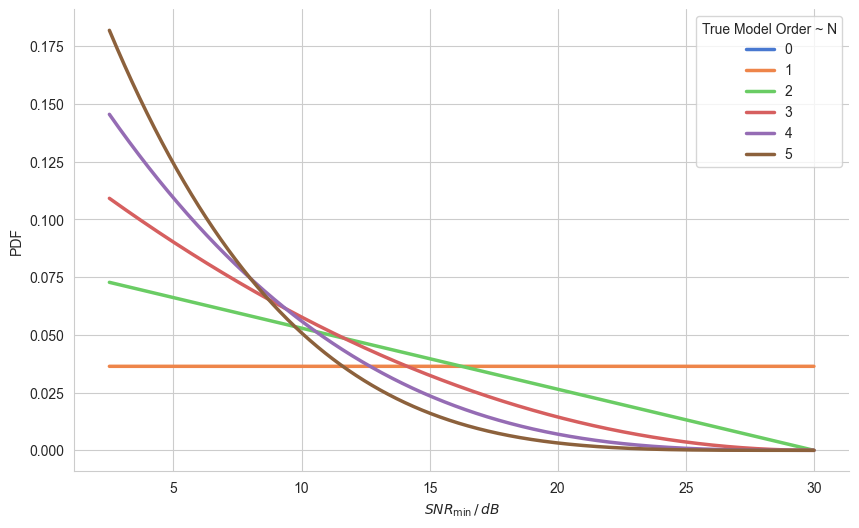
\includegraphics[width=0.5\textwidth]{figures/07_Evaluation/snr_hist/pdf_snr_min.png}}}
    \subfloat[\( \hat{f}_{\SNRmin} \)]{{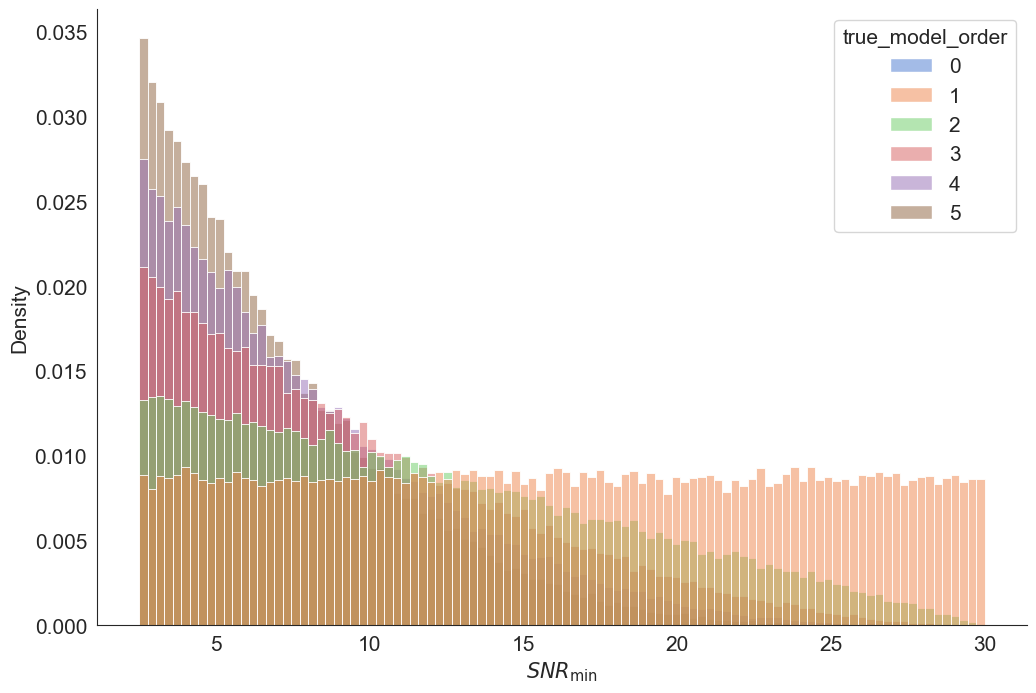
\includegraphics[width=0.5\textwidth]{figures/07_Evaluation/snr_hist/min_N.png}}}
    \newline
    \subfloat[\( f_{\SNRmax} \)]{{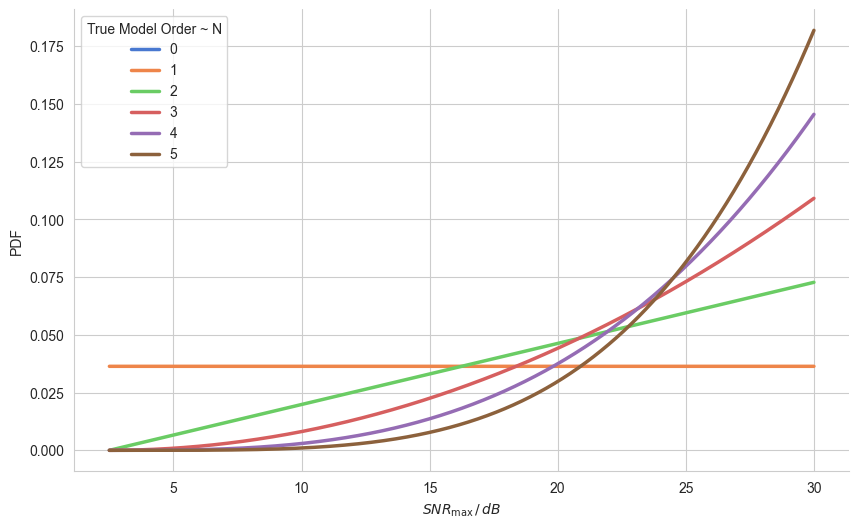
\includegraphics[width=0.5\textwidth]{figures/07_Evaluation/snr_hist/pdf_snr_max.png}}}
    \subfloat[\( \hat{f}_{\SNRmax} \)]{{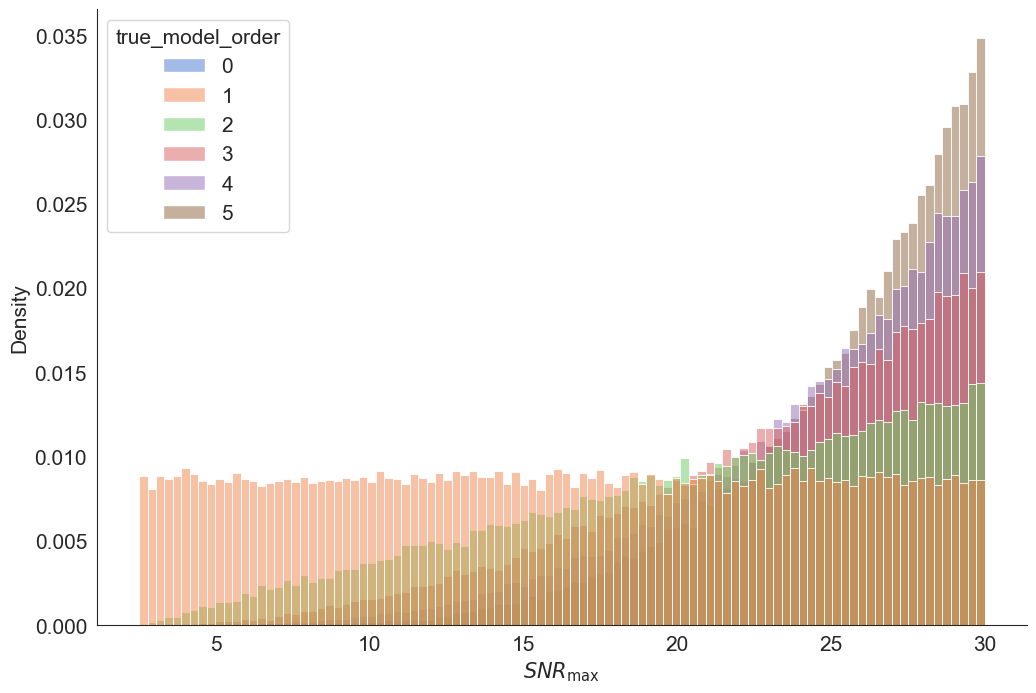
\includegraphics[width=0.5\textwidth]{figures/07_Evaluation/snr_hist/max_N.png}}}
    \caption{Theoretical \glspl{pdf} (a, c) and empirical density estimates (b, d) for \( \SNRmin \) and  \( \SNRmax \).}
    \label{fig:snr_pdf}
\end{figure}

To obtain the PDF of the \( \SIR \) distribution for \( N \geq 2 \), a convolution of the PDFs of the random variables \( \SNRmin \) and \( \SNRmax \)
is required. The convolution of the two PDFs is given by:
\begin{equation}
    f_{\SIR}(z) = \int_{-\infty}^{+\infty} f_{\SNRmax}(x) f_{\SNRmin}(z - x) \, dx
    \label{eq:sir_pdf}
\end{equation}

Numerical integration of the convolution in~\autoref{eq:sir_pdf} yielded the following PDF for \( \SIR \)~\cite[Chapter 8.2]{blitzstein2019}:
\begin{figure}[H]
    \centering
    \subfloat[\( f_{\SIR} \)]{{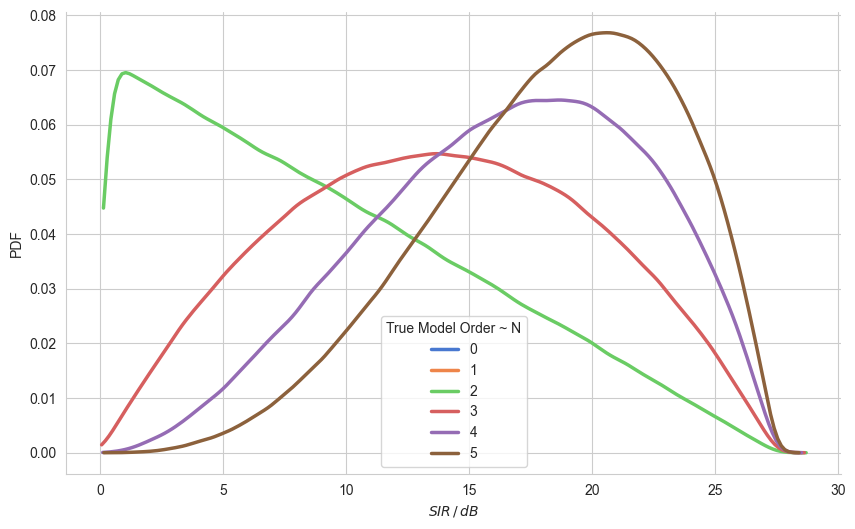
\includegraphics[width=0.5\textwidth]{figures/07_Evaluation/snr_hist/pdf_sir.png}}}
    \subfloat[\( \hat{f}_{\SIR} \)]{{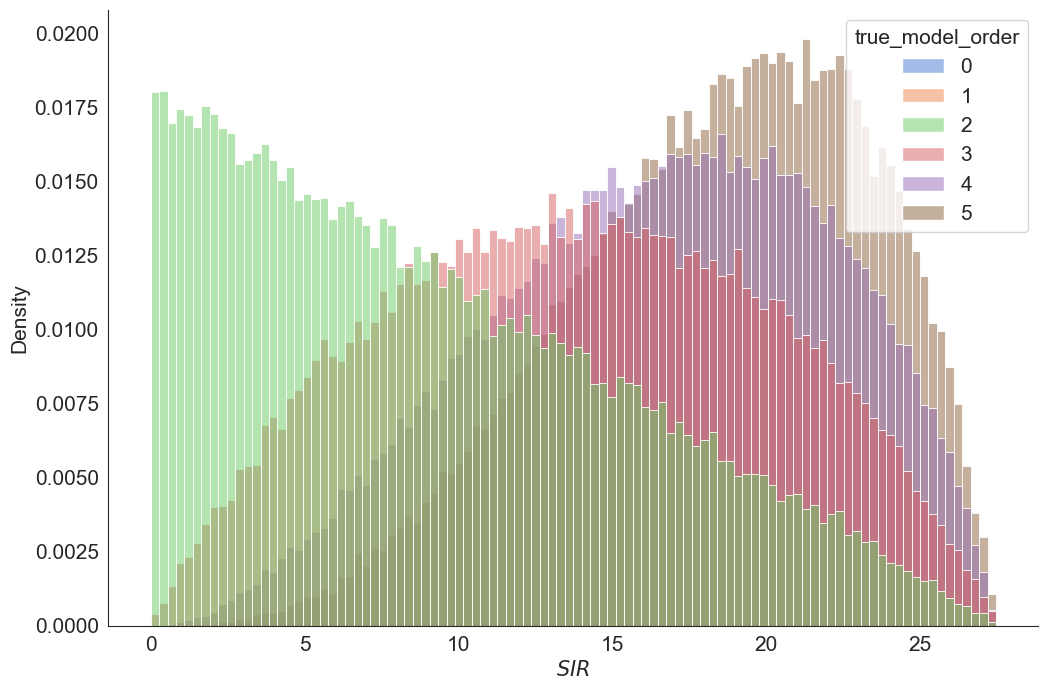
\includegraphics[width=0.5\textwidth]{figures/07_Evaluation/snr_hist/sir_N.png}}}
    \caption{Theoretical \glspl{pdf} (a) and empirical density estimates (b) for \( \SIR \).}
    \label{fig:sir_pdf}
\end{figure}
%%%%%%%%%%%%%%%%%%%%%%%%%%%%%%%%%%%%%%%%%%%%%%%%%%%%%%%%%%%%%%%%%%%%%%%%%%%%%%%%%%%%%%%%%%%%%%%%%%%%%%%%%%%%%%%%%%%%%%%%

\section{Supplementary Dataset Variations}
\label{sec:supplementary_datasets}
To further our understanding, we generated additional datasets with parameters largely mirroring those in \autoref{tab:dataset_parameters}.
These datasets, however, vary in the number of snapshots \( K \) or employ a fully sampled covariance matrix, as delineated below:

\begin{align*}
    \DKvar &\leftrightarrow  K = var. \land K \in [1, 1000]\\
    \DCoh &\leftrightarrow  \text{uses fully sampled covariance matrix}\\
\end{align*}


The sampling strategy for \( K \) within \( \mathcal{D}^{\{K_{var.},\text{Sub}\}} \) is as follows:

\[
    K_{var} =
\begin{cases}
    \text{2000 samples, increment of 1,} & \text{for } 1 < K \leq 10, \\
    \text{20000 samples, increment of 5,} & \text{for } 10 < K \leq 100, \\
    \text{20000 samples, increment of 10,} & \text{for } 100 < K \leq 200, \\
    \text{20000 samples, increment of 25,} & \text{for } 200 < K \leq 1000.
\end{cases}
\]

Post-generation, the dataset underwent uniform resampling with a step size of 25 to ensure a balanced distribution across
the spectrum of snapshots, thus providing a robust basis for model evaluation.




\chapter{Model Order Estimation}
\label{ch:ModelOrderEstimation}

\section{Introduction}
Model selection is a broad field in statistical analysis and signal processing, focusing on selecting the optimal model
from a set of candidate models based on specific criteria or metrics~\cite{costa2009}.
Within this context, \glsdesc{moe}%
\footnote{%
    Also referred to as \textit{model order selection} in the literature.
}
seeks to ascertain the most suitable number of parameters or components for fitting a model to a given dataset~\cite{barthelme2020}.\\
Classical methods for \gls{moe}, known as \glspl{ic}, aim to balance the goodness of fit of a model to the data
adversarial to its complexity by employing some form of regularization to avoid overfitting.

\subsubsection*{MOE in the Field of DOA Estimation}
In the domain of \gls{ddf}, \gls{moe} is concerned with discerning the count of incident far-field wave-fronts,
simultaneously impinging on an antenna array like a \gls{uca}.
The estimation of the model order is a crucial step in \gls{doa} estimation, as it fundamentally allows the selection
of the most likely signal model among several candidates~\cite{barthelme2020}.\\
As outlined in Section~\ref{sec:sub:subspaces}, the model order \( N \) corresponds to the rank of the signal subspace
\( \bfm{U}_S \) and also equals the number eigenvalues that are different from the smallest eigenvalue.
This assumption holds when all \( N \) incoming signals are uncorrelated and thus linearly independent and \( \C \rightarrow \bfm{C}_x \),
which can be assumed to be true for \( K \gg M \)~\cite{trees.ch7}.\\
As mentioned earlier, super-resolution algorithms such as \gls{music}, elaborated upon in the previous
chapter, rely on an accurate estimate of the model order \( \NPred \) for effective subspace decomposition (\( \bfm{U} = \bfm{U}_S \oplus \bfm{U}_N \)).
Furthermore, the operator of a \gls{ddf} system or a sophisticated policy-selection algorithm might use the condition
\( \NPred \overset{?}{>} 1 \) as a criterion to select the most suitable direction finding algorithm.


\section{Classical Information Criteria}
\label{sec:ClassicalInformationCriteria}
The \gls{aic} and the \gls{mdl}, both classical \glspl{ic},
are frequently employed for \gls{moe}. They were first utilized to determine the number of impinging wavefronts by introducing
a convenient reparametrization of the maximum likelihood estimate of the underlying signal model in~\cite{mdlAndAic}.
The general form of the log-likelihood function for our data model is given by:

\begin{equation}
    \NPred=\underset{n \in \NSet}{\argmax} \ln \left(p_{n}\left(\bfm{x} ; \widehat{\bfT}, \C, \widehat{\sigma}_\eta^2\right)\right)+ c(n)
    \label{eq:max_likelihood}
\end{equation}

The maximum likelihood estimate is denoted by \( p_{n}(\cdot) \), and \( c(n) \) is a regularization term that penalizes
large model orders~\cite{barthelme21sub}.
The reparametrization of the likelihood estimate significantly increases the simplicity of the
model order estimation problem, as it allows the likelihood function to be solely expressed in terms of the eigenvalues of the
covariance matrix \( \C \).
The essence of these classical approaches to \gls{moe} lies in discerning the set of eigenvalues from a covariance matrix that significantly diverge
from a tightly grouped cluster with low variance, which is centered around the noise variance \( \sigma^2_{\eta} \).
The aim is to reduce the variance among the smallest \( M - n \) eigenvalues, while adversarially penalizing large
values for \( M - n \) to avoid overfitting.\\


Central to both criteria is the ratio between the arithmetic mean \( \am(\bfL_n) \) and the geometric mean
\( \gm(\bfL_n) \) of the \( M - n \) smallest eigenvalues.\\
It is expressed as:
\begin{equation}
    \am(\bfL_n) \coloneqq \frac{1}{M-n} \sum_{i=n+1}^{M} \lambda_i
\end{equation}

Similarly, the geometric mean for these eigenvalues is:
\begin{equation}
    \gm(\bfL_n) \coloneqq \sqrt[M-n]{\prod_{i=n+1}^{M} \lambda_i}
\end{equation} %TODO: starting idx??

The ratio of the geometric mean to the arithmetic mean equals one when all eigenvalues are identical, reflecting a
uniform distribution—this would be the case for an ideally estimated subspace of \gls{awgn}.
A higher ratio indicates a departure from a uniform distribution in the set of considered eigenvalues, thus highlighting
the presence of signal eigenvalues. Both \glspl{ic} exploit this relationship, seeking the subset of
eigenvalues that most closely mirror a uniform distribution, and thereby distinguishing the noise subspace
from the signal subspace \( \bfm{U} = \bfm{U}_S \oplus \bfm{U}_N \)~\cite{meyer}.\\
For ease of reference and clarity, we define \( \NSet \) as the set of potential model orders. Specifically,
\( \NSet \coloneqq \{1, \ldots, N_{\max}\} \), where \( N_{\max} = M - 1\) is the maximum possible number of incoming signals%
\footnote{
In practice, \( N_{\max} \) is often set to a lower value to simplify computations, since the likelihood of encountering
up to \( M - 1 \) incoming signals is often negligible.
}.\\

\subsubsection{Akaike Information Criterion (AIC)}

For each potential model order \(n \in \NSet \), the AIC criterion \( \bfm{\mathrm{AIC}} \) can be represented as~\cite{mdlAndAic}:
\begin{equation}
    \bfm{\mathrm{AIC}}[n] = - 2 \cdot \underbrace{{\ln \left(\frac{\gm(\bfL_n)}{\am(\bfL_n)}\right)}^{K(M - n)}}_{log-likelihood} + \underbrace{2n(2M - n)}_{\text {regularization term }} \quad \text{for each } n \in \NSet
    \label{eq:AIC}
\end{equation}


Employing our previous notations, \( M \) denotes the number of antennas and \( K \) the snapshot count.
The estimated model order \( \NPred_\mathrm{AIC} \) can then be calculated as:

\begin{equation}
    \NPred_\mathrm{AIC}=\underset{n \in \NSet}{\argmin}\{ \bfm{\mathrm{AIC}}[n] \}
    \label{eq:AIC_argmin}
\end{equation}

\subsubsection{Minimum Description Length (MDL)}
The MDL criterion is formulated as~\cite{mdlAndAic}:
\begin{equation}
    \bfm{\mathrm{MDL}}[n]=  - {\ln \left(\frac{\gm(\bfL_n)}{\am(\bfL_n)}\right)}^{K(M - n)} + \frac{1}{2} n(2 M-n) \ln (K)
    \label{eq:MDL}
\end{equation}

The estimated model \( \NPred_\mathrm{MDL} \) order can than be calculated in the same fashion as in \autoref{eq:AIC_argmin}.\\
Both \gls{aic} and \gls{mdl} are based on the same principle, but differ in their approach to penalizing large model orders.
While both criteria linearly penalize the model order \( n \), \gls{mdl} additionally tends to favor smaller model orders given
an increasing number of snapshots.
\gls{mdl} tends to yield a more consistent model order estimate than \gls{aic}, which is more prone to overfitting in non-subsampled
scenarios~\cite{mdlAndAic, barthelme2020}.\\


\subsubsection{A Practical Example of Model Order Estimation}
\autoref{fig:aic_mdl_criteria} illustrates the application of \gls{aic} and \gls{mdl} to predict the model order for
a scenario, drawn from the dataset \( \DMain_{(\text{test})} \), with \( M = 9 \) antennas and \( K = 100 \) snapshots
and the use of the incoherent covariance matrix \( \Csub \).

\begin{figure}[H]
    \centering
    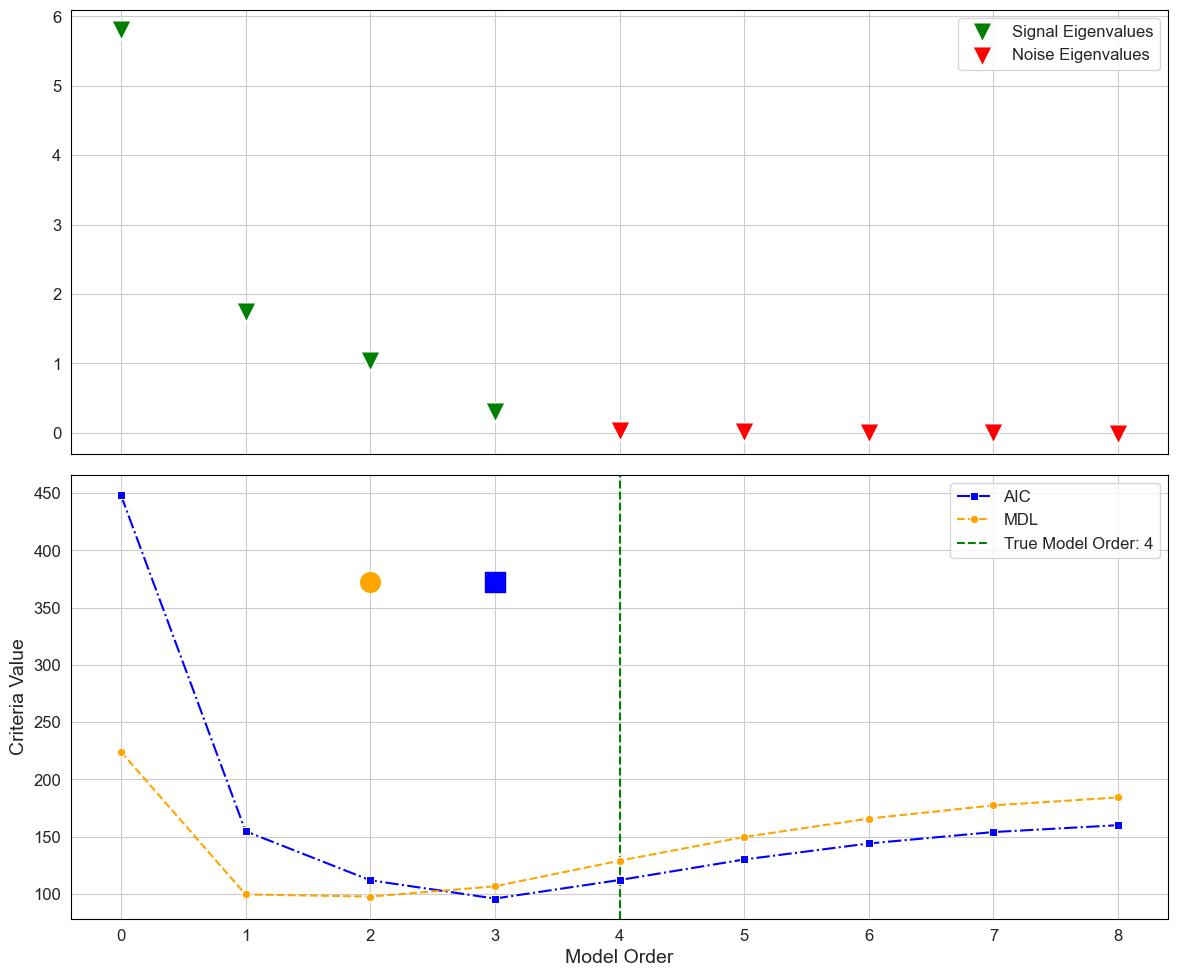
\includegraphics[width=0.8\textwidth]{figures/04_ModelOrderEstimation/aic_mdl_criteria.png}
    \caption{A working example of the \gls{aic} and \gls{mdl} estimators.}
    \label{fig:aic_mdl_criteria}
\end{figure}

For this setup, the \gls{aic} predicted a model order \( \NPred_\mathrm{AIC} = 3 \), while \gls{mdl} estimated
\( \NPred_\mathrm{MDL} = 2 \), reflecting the impact of the more pronounced regularization term in \gls{mdl}.
The underfitting of the model order prediction is not expected, given the actual \gls{snr} and \gls{sir} values, with \( \mathrm{SIR}_{\max} = 10.86 \, \text{dB} \)
and \( \mathrm{SNR}_{\min} = 14.77 \, \text{dB} \). \\
The reason for the underwhelming performance of the \gls{aic} and \gls{mdl} criteria in this
scenario is due to effects of sub-sampling and the ``limited'' number of snapshots \( K \).
The former effect seems to be the primary reason for a pronounced bias towards underestimating the model order.
These repercussions will be the subject of further investigation in \autoref{sec:challenges_moe} and \autoref{ch:evaluation_results}.



\section{Exponential Fitting Test (EFT)}
\label{sec:eft}
\subsection{Introduction}
The \glsdesc{eft}, first introduced by~\cite{eft} in 2007, marks an algorithmical paradigm shift the domain of \gls{moe}
the \gls{eft} aims to directly detect gap a gap between the noise and signal eigenvalues, rather than relying on
the indirect approach of discerning a uniform distribution among the noise eigenvalues.
It was designed to overcome the limitations of traditional methods when dealing with non-coherent sources and a small
number of snapshots, all while maintaining computational complexity comparable to the \glspl{ic} discussed in \autoref{sec:ClassicalInformationCriteria}.
The \gls{eft} leverages the observation that the descendingly ordered noise eigenvalues approximately exhibit exponential decay.
The algorithm seeks to robustly predict the model order by identifying discrepancies
that exceed a predetermined threshold between the observed eigenvalues and the
anticipated exponential decay curve, thereby effectively distinguishing between signal and noise. \\

Despite subsequent enhancements to the \gls{eft} as detailed in~\cite{costa2007} and~\cite{costa2009}, the original version
has been implemented as a baseline for comparative analysis against classical methods like \gls{aic} and \gls{mdl} and
the \glspl{dnn} architectures explored in this thesis.\\

\subsection{Algorithm}
\subsubsection*{Estimating the Decay Coefficients}

The \gls{eft} algorithm employs a recursive approach to model the exponential decay pattern of noise eigenvalues.
This decay is represented by\footnote{To distinguish between the predicted and observed eigenvalues, of the
\textit{estimated} covariance matrix \( \C \), the former are denoted as \( \hat{\lambda} \), while the estimated
observed eigenvalues will be denoted without their hat \( \widehat{\bullet} \).}:
\begin{equation}
    \hat{\lambda}_i = \lambda_1 \cdot {q(M, K)}^{i-1} \quad \text{for } i \in \NSet, \; q \in (0, 1)
    \label{eq:eft_decay_coeff}
\end{equation}
In \autoref{eq:eft_decay_coeff}, \( \lambda_1 \) represents the largest eigenvalue in a noise-only scenario, and \( q(M, K) \) is the decay
coefficient, which varies based on the number of antennas \( M \) and the number of snapshots \( K \).
The challenge lies in accurately determining the decay coefficient \( q : (M, K) \rightarrow \mathbb{R} \) to estimate
exponential decay of the noise eigenvalues.

\cite{eft} derived a method to estimate \( q \) based on the first order approximation of the noise variance \( \sigma^2_{\eta} \)
aussiming a noise-only scenario:
\begin{equation}
    \sigma^2_{\eta} \approx \frac{1}{M} \sum_{i=1}^{M} \lambda_i
    \label{eq:eft_noise_variance}
\end{equation}

Through a series of mathematical transformations, detailed in~\cite{eft}, a relation involving \( q \) is formulated:
\begin{equation}
    \frac{M+K}{M K} = \frac{(1-q)\left(1+q^M\right)}{\left(1-q^M\right)(1+q)}
\end{equation}

Solving this equation for \( q \) involves using a substitution \( q = \exp(-2a) \) and subsequently solving the
resultant cubic equation for \( a \):
\begin{equation}
    a=\sqrt{\frac{1}{2}\left\{\frac{15}{M^2+2}-\sqrt{\frac{225}{\left(M^2+2\right)^2}-\frac{180 M}{K\left(M^2-1\right)\left(M^2+2\right)}}\right\}} .
    \label{eq:eft_decay_coefficient}
\end{equation}

\subsubsection*{Iterative Eigenvalue Prediction and Comparison}
Following the calculation of the pre-computable decay coefficient \( q \), the predictive process of the \gls{eft} algorithm
begins by assuming the smallest observed eigenvalue \( \lambda_M \) to be part of the noise subspace,
setting the initial noise subspace dimension \(  p= 1 \). The process iteratively predicts each subsequent
eigenvalue according to the assumed exponential decay pattern, expanding the candidate noise subspace and recalculating
\( \hat{\lambda}_{M-p} \) from the updated estimate of the noise variance \( \widehat{\sigma}^2_{\eta} \).
This evaluation continues until a significant mismatch between the observed eigenvalue and the predicted noise profile is detected.
The predicted eigenvalue \( \hat{\lambda}_{M-p} \) is calculated as:
\begin{equation}
    \hat{\lambda}_{M-p} = \frac{1 - q(M, K)}{1 - {q(M, K)}^{p + 1}} \cdot \underbrace{\sum_{i=0}^{p}\lambda_{M-i}}_{(p+1)\widehat{\sigma}^2\eta}
    \label{eq:eft_predicted_eigenvalue}
\end{equation}


\subsubsection*{Hypothesis Testing}

With each iterative step of the \gls{eft} process, two competing hypotheses are considered for the eigenvalues under
examination:

\begin{align}
    \mathcal{H}_{p+1} &: \lambda_{M-p} \in \bfL_\eta \label{eq:hypothesis_noise} \\
    \widetilde{\mathcal{H}}_{p+1} &: \lambda_{M-p} \in \bfL_S \label{eq:hypothesis_signal}
\end{align}

Starting with the pair \( (\lambda_{M-1}, \hat{\lambda}_{M-1}) \), the relative distance between each of the
theoretical noise eigenvalues and their corresponding observed eigenvalue is computed. This difference is then assessed
against a predefined threshold value \( \tau_n \), which scales with the eigenvalue index. The condition for
determining the hypothesis to accept is as follows:

\begin{equation}
    \text{accept } \left\{
        \begin{array}{ll}
            \mathcal{H}_{p+1}, & \text{if } \left|\frac{\lambda_{M-p} - \hat{\lambda}_{M-p}}{\hat{\lambda}_{M-p}}\right| = \epsilon_n \leq \tau_n, \\
            \widetilde{\mathcal{H}}_{p+1}, & \text{otherwise}.
        \end{array}
    \right.
    \label{eq:threshold_condition}
\end{equation}


If the relative difference falls within the threshold, the eigenvalue is classified as noise; otherwise, it is considered
to be an eigenvalue of the signal subspace.
The process iterates, comparing each predicted noise eigenvalue with its observed counterpart,
until a relative error \( |\epsilon| > \tau \) is encountered, signifying a departure from the noise eigenvalue pattern and the
detection of the smallest signal eigenvalue.\\
\autoref{eq:threshold_condition} as proposed in \cite{eft} could classify a \( (\lambda_n, \hat{\lambda}_n) \) pair
as signal if the predicted eigenvalue is smaller than its observed counterpart, which seems unsound. Thus, the signed
relative error \( \epsilon \) should be used instead of the absolute relative error \( |\epsilon| \) in \autoref{eq:threshold_condition}.
The estimated dimension of the noise subspace \( \widehat{p} \) is thus determined to be the value
of \( p \) at which the hypothesis \( \mathcal{H}_{p+1} \) is rejected in favor of \( \widetilde{\mathcal{H}}_{p+1} \). Consequently, the estimated
model order, is given by \( \NPred = M - \widehat{p} \), marking the completion of the \gls{eft} process.\\

\begin{figure}[H]
    \centering
    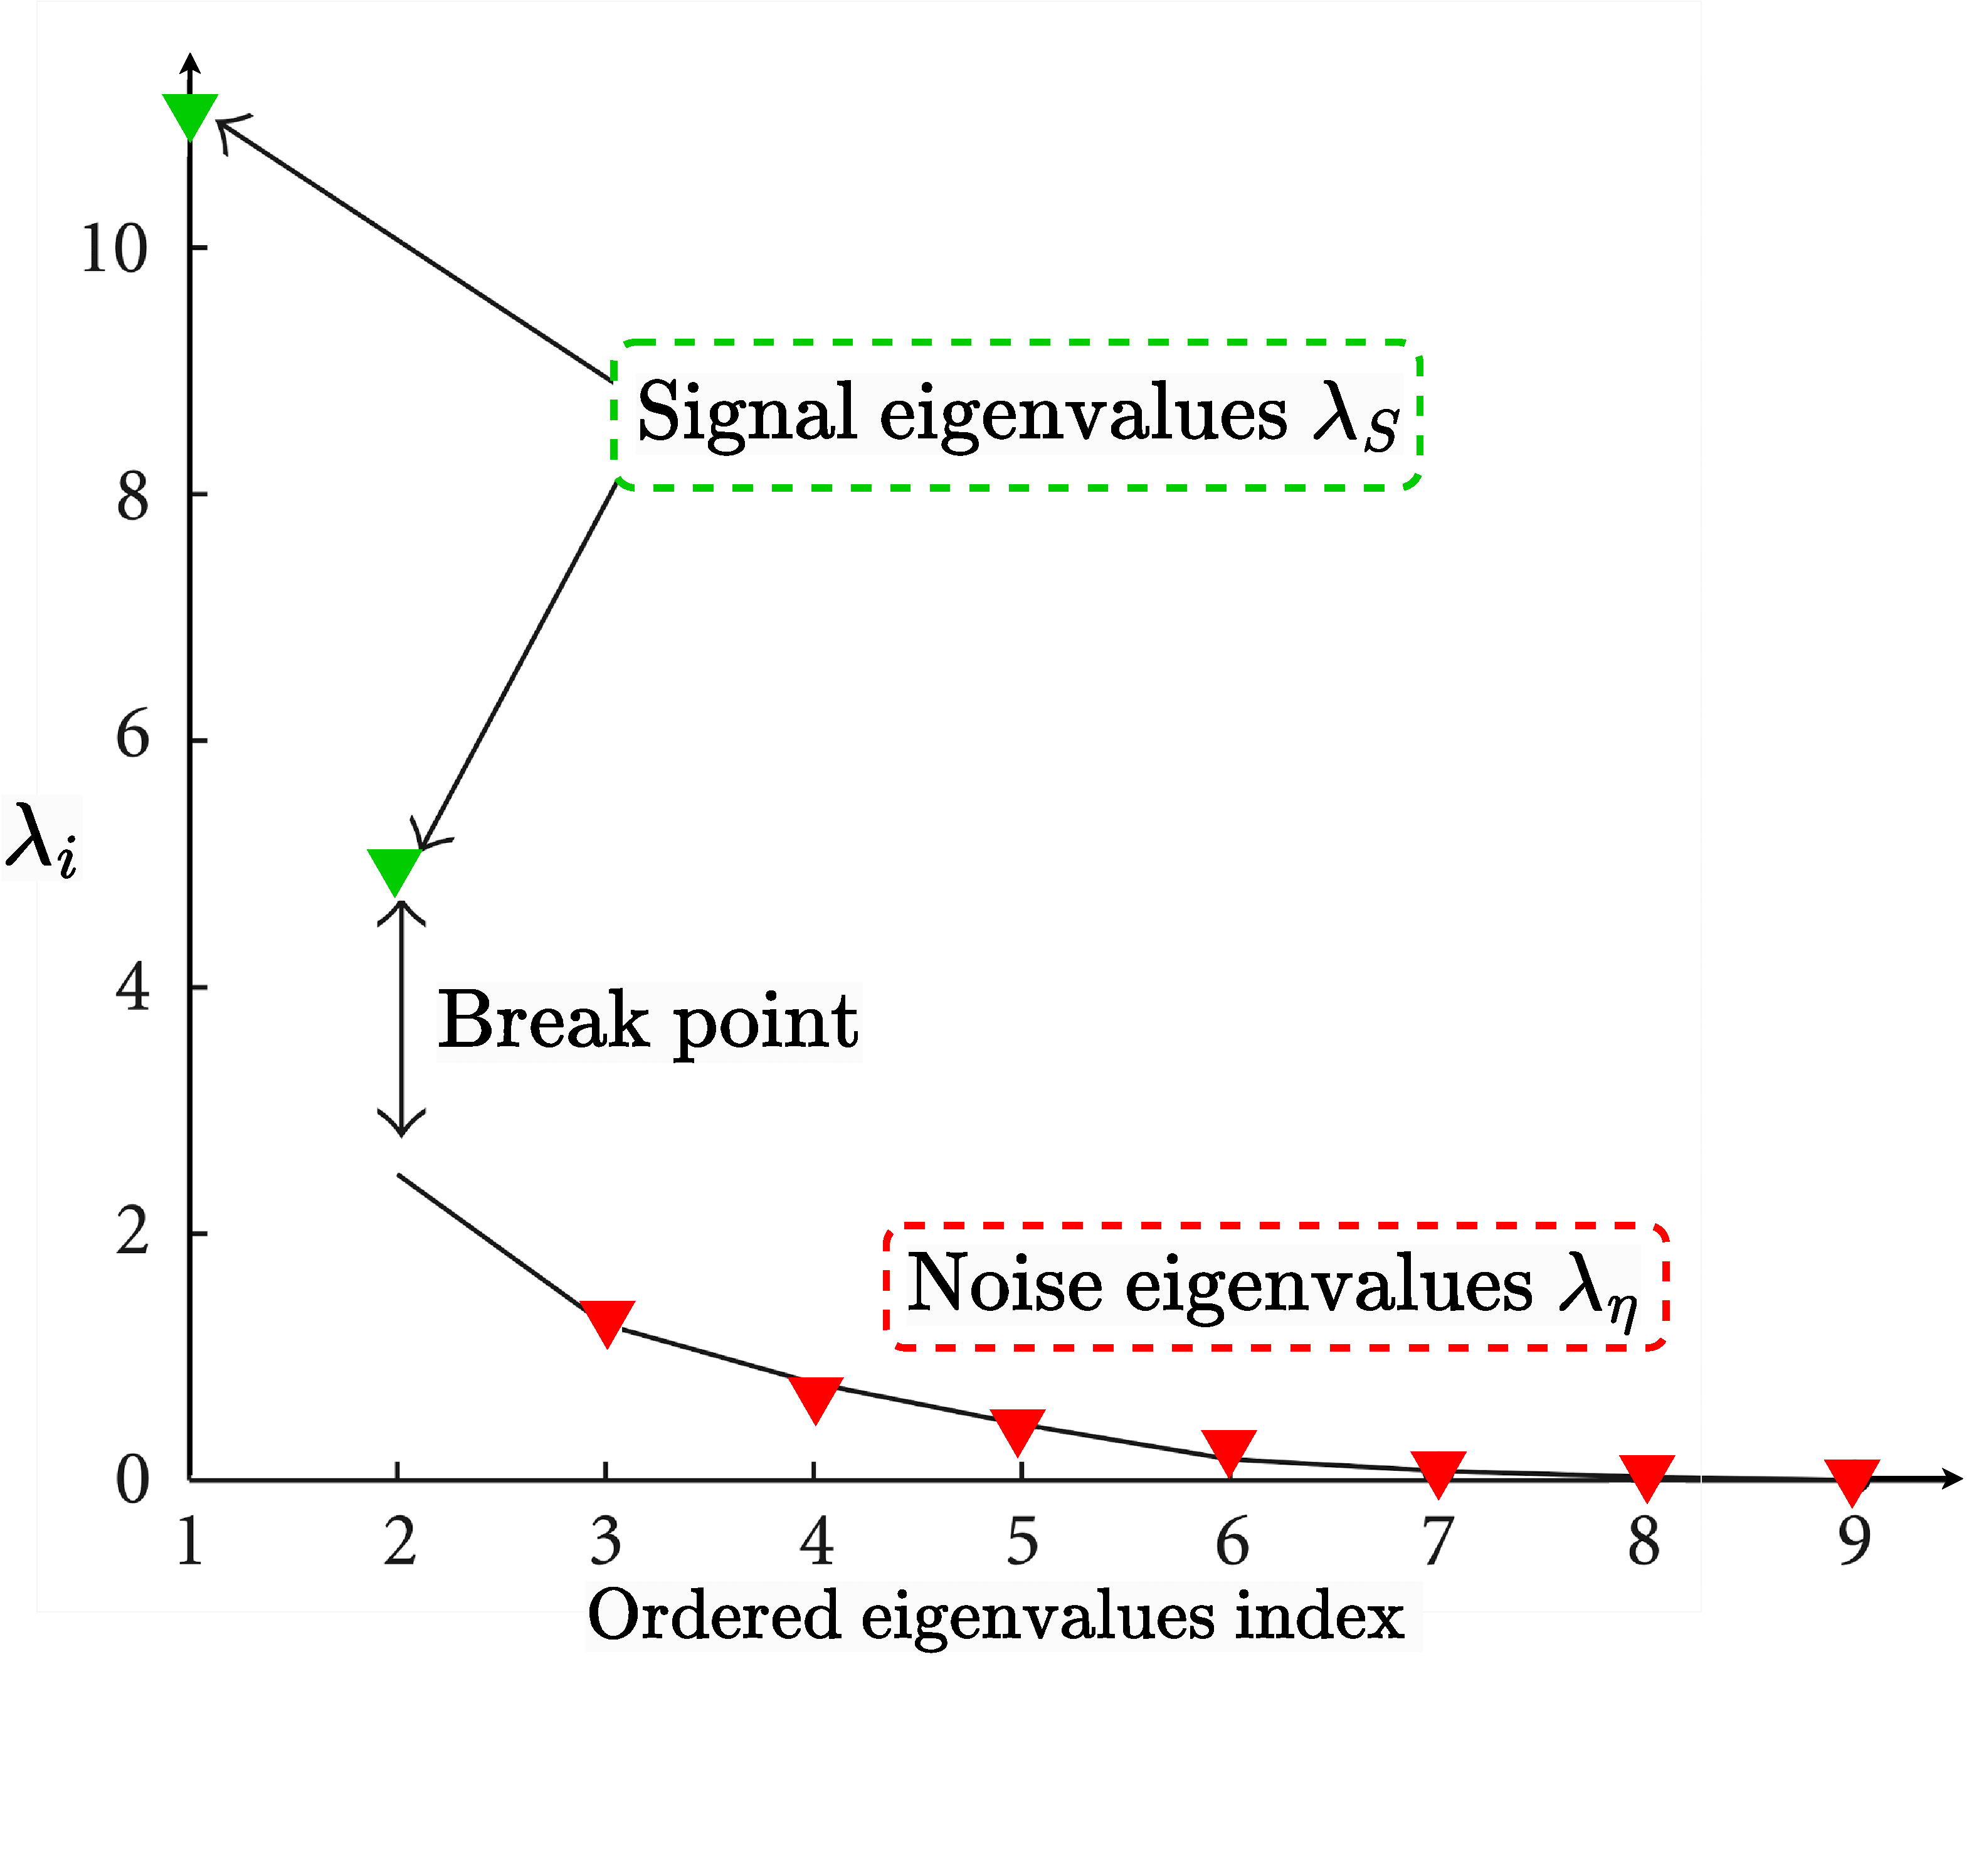
\includegraphics[width=0.55\textwidth]{figures/04_ModelOrderEstimation/eft_scheme.pdf}
    \caption{Conceptual illustration of the \gls{eft} technique-adapted from~\cite{eft}.}
    \label{fig:eft_scheme}
\end{figure}

\autoref{fig:eft_scheme} illustrates the \gls{eft} process for a scenario with \( M = 9 \) antennas and a model order of
\( N = 2 \). The eigenvalue distribution in the figure exposed the discrepancy between the noise and signal
eigenvalues.
For a given \( p = 7\), the hypothesis \( H_{7 + 1} \) is rejected in favor of \( \widetilde{H}_{7 + 1} \), revealing
the smallest signal eigenvalue to have the index \( M - \widehat{p} = \NPred = 2 \). This corresponds to the actual model order.


\subsection{Threshold Calculation}
Similar to the approach in the original study~\cite{eft}, the threshold values \( \epsilon_n \) were calculated based on
predefined false positive rates \( \bfm{F} \) for each possible model order \( n \in \NSet \).
The original study employed a single false positive rate of \( 1 \% \). However, this may not be optimal as eigenvalues
with higher indices are more likely to be checked, increasing the likelihood of false positives for these indices due to
the increased check frequency.

\begin{algorithm}[H]
\label{alg:eft_threshold_calculation}
\caption{EFT Threshold Calculation}
\DontPrintSemicolon
\KwIn{\;
\quad \( \bfm{E} \): Relative errors, calculated as per \autoref{eq:threshold_condition} on the train set\;
\quad \(\bfm{F}\): List of desired false positive rates for each potential signal eigenvalue\;
\quad \(N_{\max}\): Max model order}
\KwOut{\;
\quad \(\bfm{\tau}\): List of threshold values}

\SetKwFunction{FMain}{CalculateEFTThresholds}
\SetKwProg{Fn}{Function}{:}{}
\Fn{\FMain{\(\bfm{E}\), \(\bfm{F}\), \(N_{\max}\)}}{
    \(\bfm{\tau} \gets\) empty list\;
    \For{\(i \gets 0\) \KwTo \(N_{\max}\)}{
        \(\bfm{S} \gets \bfm{E}\) where \( N \leq i\)\;
        \(\bfm{S}_{\text{sorted}} \gets\) sort(\(\bfm{S}[:, i]\))\;
        \(L \gets\) length(\(\bfm{S}_{\text{sorted}}\))\;
        \(\mathrm{Idx} \gets \min(\left\lfloor(1 - \bfm{F}[i]) \cdot L\right\rfloor, L - 1)\)\;
        \(\tau_i \gets \bfm{S}_{\text{sorted}}[\mathrm{Idx}]\)\;
        Append \(\tau_i\) to \(\bfm{\tau}\)\;
    }
    \KwRet \(\bfm{\tau}\)\;
}
\end{algorithm}

Utilizing algorithm \autoref{alg:eft_threshold_calculation}, the following treshold values \( \bfm{\tau} \) were calculated
for the the respective false positive rate

\begin{table}[h]
    \centering
    \caption{Calculated EFT tresholds}
    \begin{tabular}{ccc}
    \toprule
    \( n \:/\: \NPred \) & FPR & \( \tau \) \\
    \midrule
    0 & 0.1 & 0.021 \\
    1 & 0.084 & 0.485 \\
    2 & 0.064 & 0.591 \\
    3 & 0.048 & 0.716 \\
    4 & 0.048 & 0.836 \\
    5 & 0.048 & 0.981 \\
    \bottomrule
    \end{tabular}
    \label{tab:eft_thresholds}
\end{table}

\subsubsection*{Conclusion}

\textbf{Threshold Adjustment and Bias Control:} The EFT aims for a delicate balance between the false
positive rate and the false negative rate, by accordingly adjusting the threshold values \( \tau_n \) for each potential
signal eigenvalue. This enables the EFT to explicitly control potential biases for over- or underestimation.
This balance is inherently tied to the careful selection and optimization of the threshold values
\( (\tau_1, \ldots, \tau_{M-1}) \), which introduce a degree of subjectivity but also a potentially
unwanted dependence that is not present in the parameter-free methods \glspl{ic}.\\
The procedure of selecting the threshold values should be invesiagted further. The following approaches could be considered:
\begin{itemize}
    \item Introduce an optimization process that considers the false negative rate in addition to the false positive rate.
    \item Investigate the choices of different false positive rates to compensate for the increased checking frequencies of
    eigenvalues with higher indices.
    \item After indentifying a suitable set of threshold values, utilize an objective driven optimization process to finetune
    the values. Empirical evidence which was gathered during the optimization of a single threshold value, indicates that
    the optimization problem is at least partially convex. Rather than optimizing all treshold values simultaneously,
    the optimization could be performed sequentially, starting with the threshold value for the smallest potential signal
    eigenvalue.~\autoref{fig:eft_treshold_optim} depicts the plot of the optimization process for a single threshold value.
\end{itemize}
%TODO Adapt plot!
\begin{figure}[H]
    \centering
    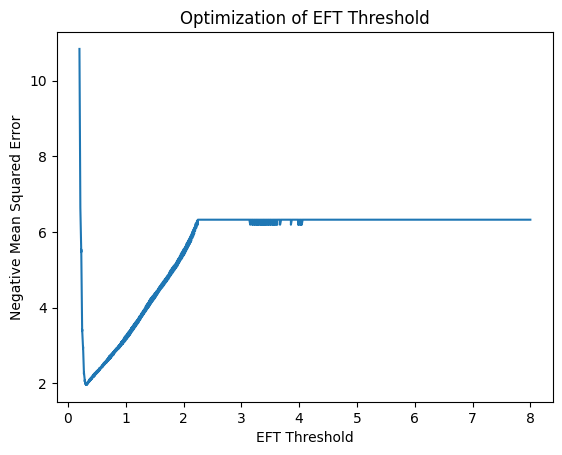
\includegraphics[width=0.5\textwidth]{figures/04_ModelOrderEstimation/eft_treshold.png}
    \caption{Optimization of a single EFT threshold value, where all \( \tau_n \) in \( \bfm{\tau} = \tau \)}
    \label{fig:eft_treshold_optim}
\end{figure}
The tresholds in \autoref{tab:eft_thresholds} differ significantly from the values which were identified in~\cite{eft}.
For \( N_{\max} = 4 \), the original study identified the following threshold values:
\[
    \bfm{\tau} = \left[26.34, 3.647, 1.238, 0.6336 \right]
\]
The divergence between the two sets of threshold values has not been subject to further scrutiny, as the EFT estimators
demonstrated superior performance compared to the AIC and MDL estimators.\\
Additionally, the transferability of these optimized threshold values to different scenarios has yet to be ascertained.
It has been observed that the EFT, with thresholds tailored to a dataset featuring a static snapshot count \( K = 100 \),
exhibited superior performance over the AIC and MDL when applied to a dataset with a variable snapshot count \( K \in [1, 1000] \).
Further details on this comparison are presented in \autoref{sec:influence_num_snapshots}.\\

\textbf{Computational Complexity:} As per~\cite{eft}, the computational complexity of the EFT is on par with that of AIC
and MDL. This assertion is presumably based on the shared requirement of these methods for an eigenvalue decomposition of
the covariance matrix. However, the EFT necessitates considerably fewer computations for the predictive steps, which are
contingent on the eigenvalues. The only computations required at runtime are:

\begin{itemize}
    \item In Equation \ref{eq:eft_predicted_eigenvalue}, the computation involves the summation of the assumed noise
    eigenvalues \( \bfL_\eta \), followed by a multiplication with the precomputed fraction for each potential model order.
    \item In Equation \ref{eq:threshold_condition}, the computation involves \( N_{\max} \) divisions and comparisons.
\end{itemize}

This computational requirement is significantly less than that of the AIC and MDL criteria, which necessitate the
computation of the logarithm of the geometric and arithmetic mean of the eigenvalues, in addition to subsequent
exponentiation for each potential model order.

\textbf{Specific Design for Incoherent Sources:} Tailored to perform well in the presence of incoherent sources,
the EFT's efficacy in environments with coherent sources or multipath interference has not been evaluated.

\textbf{Implementation Caution:}
The Python implementation of the EFT for this thesis presents some inconsistencies when compared to the original EFT
algorithm. A particular point of ambiguity is the calculation of the decay coefficient \( q \), which is not clearly
defined in the original study as to whether it depends on the number of snapshots \( K \) and the noise subspace
dimension \( p \), or on the number of snapshots \( K \) and the number of antennas \( M \).
The notation \( q : (p + 1, K) \rightarrow \mathbb{R} \) versus \( q : (M, K) \rightarrow \mathbb{R} \) is used in~\cite{eft}'s
equivalent to \autoref{eq:eft_predicted_eigenvalue} and is the source of this uncertainty.\\
Both possible versions have
been implemented, but the version with \( q(p+1, N) \) tends to result in estimated exponential decay profiles which
exhibit an unexpected curvature for an exponential function, as depicted in \autoref{fig:eft_coeff_comparison}.
Therefore the version with \( q(M, N) \) is used in this thesis.\\
Another point of ambiguity is the estimation of the noise variance \( \widehat{\sigma}^2_{\eta} \) in \autoref{eq:eft_predicted_eigenvalue}.
According to~\cite{eft}, the noise variance is estimated as the arithmetic mean of the \( p + 1 \) smallest eigenvalues,
this means that \( \lambda_n \) is utilized in the estimation of the noise variance, which will then be used to calculate
\( \hat{\lambda}_n \). This might introduce a bias towards underestimating the model order.

\begin{figure}[H]
    \centering
    \subfloat[]{{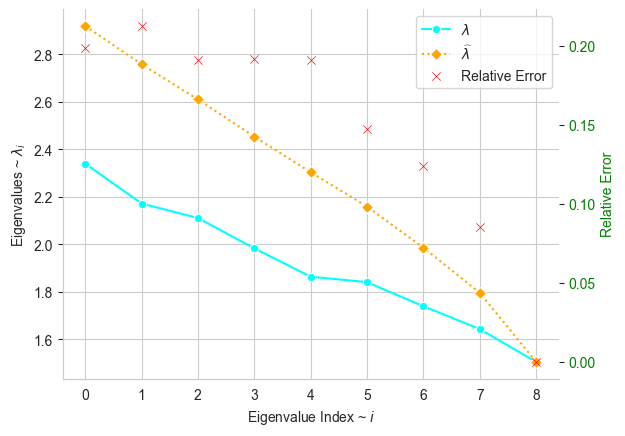
\includegraphics[width=0.45\textwidth]{figures/04_ModelOrderEstimation/eft_wrong_coeff.png}}}
    \subfloat[]{{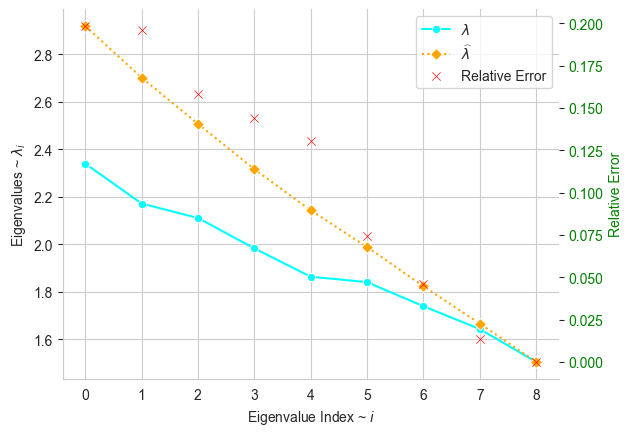
\includegraphics[width=0.45\textwidth]{figures/04_ModelOrderEstimation/eft_correct_coeff.png}}}
    \caption{Comparison of the EFT's predicted eigenvalues, with the decay coefficient \( q \) calculated with \( q(p+1, N) \) (a) and \( q(M, N) \) (b).}
    \label{fig:eft_coeff_comparison}
\end{figure}

\newpage{}
\section{Challenges of Eigenvalue Based MOE}
\label{sec:challenges_moe}

\subsection{Degradation of the Eigenstructure through Sub-Sampling}

The application of classical \glspl{ic} such as \gls{aic} and \gls{mdl} for model order estimation critically depends on the
soundness of the re-parameterization of the maximum likelihood function introduced in~\autoref{eq:max_likelihood}.
While robust and effective for coherently sampled covariance matrices, this methodology loses its validity
due to the severely increased challenge in capturing the true eigenstructure of the covariance matrix \( \bfm{C}_x \)
when sub-array sampling is employed~\cite{barthelme21sub}.

Barthelme et al.~\cite{barthelme21sub} asserted that the eigenstructure of the sub-sampled covariance matrix \( \Csub \)
can no longer be decomposed into signal and noise subspaces when the model order \( N \) exceeds the number of RF
chains \( L \).\\
In contrast, Meyer~\cite{meyer} demonstrated the convergence of \( \Csub \rightarrow \bfm{C}_x \) as \( K \rightarrow \infty \).
It is thus obvious that the sub-sampled covariance matrix's eigenstructure must still posses the capacity to encode
the coveted information (\( \{ \bfT_n :\, n \in \{1, \ldots, N\} \} \)). \\
This convergence, however, unfolds asymptotically and at a pace that challenges its practical utility in real-world scenarios.

The progression from theoretical considerations to empirical observations underscores the practical dilemmas posed by
sub-array sampling. The fidelity with which \( \Csub \) mirrors \( \bfm{C}_x \) is notably compromised, as it not only
loses positive semi-definiteness but also introduces a broader dispersion of the noise eigenvalues \( \bfL_{\eta} \).
This dispersion deviates from their expected individual normal distributions around the noise variance \( \sigma^2_\eta \)~\cite[Chapter 6]{meyer}.

These revelations prompt critical inquiry into the manifestation and progression of information loss within the
eigenstructure of \( \Csub \), especially under finite snapshot conditions. \\
Does this information loss occur abruptly with the emergence of negative eigenvalues, or does it manifest more gradually,
with eigenvalues slowly diverging from those of \( \bfm{C}_x \)?


\subsubsection{Distribution of the noise eigenvalues}
\label{subsub:noise_eigval_distrib}
\begin{figure}[H]
    \centering
    \subfloat[]{{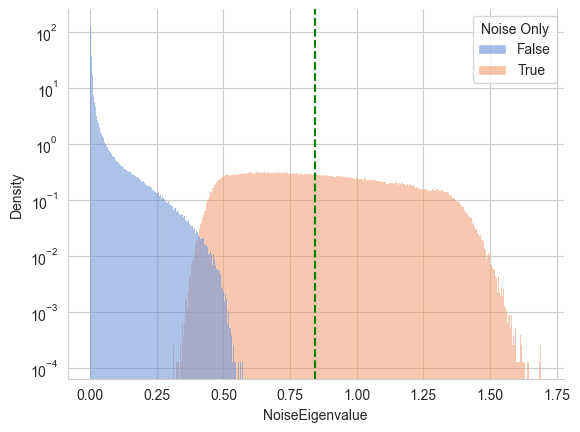
\includegraphics[width=0.5\textwidth]{figures/04_ModelOrderEstimation/noise_eigval_distrib.png}}}
    % \hspace{0.5cm}
    \subfloat[]{{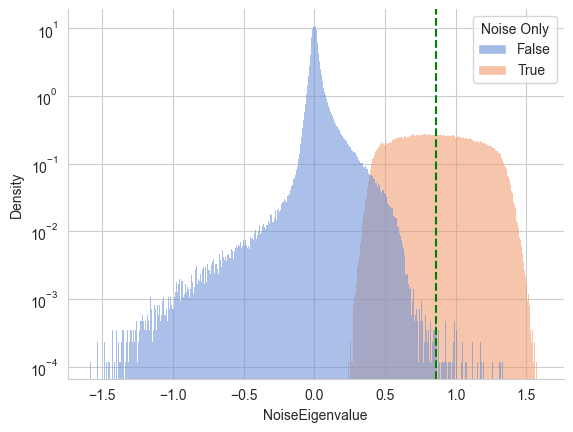
\includegraphics[width=0.5\textwidth]{figures/04_ModelOrderEstimation/noise_eigval_distrib_sub.png}}}
    \caption{Density estimates of noise eigenvalues of the full (a) and sub-sampled (b) covariance matrices, and \( K = 100 \).}
    \label{fig:noise_eigval_distrib}
\end{figure}

\autoref{fig:noise_eigval_distrib} depicts the density estimates of noise eigenvalues for both full and sub-sampled
covariance matrices, given a set number of snapshots \( K = 100 \).
The dataset was generated with a specified noise level of \( P_\eta = -120 \, \si{\deci\bel}_{(\si{\micro\volt})} \),
equating to a noise variance of \( \sigma^2_\eta = 1 \si{\micro\volt\squared} \). \\
The theoretical expectation for the distribution of the noise eigenvalues is given by~\autoref{eq:eigval_superimposed} and
assumes normally distributed noise eigenvalues around \( \sigma^2_\eta \).\\
In the noise-only case, where no signals are present (\( N = 0 \)), the orange distributions indeed aligns with this prediction.
However, the blue distribution, representing scenarios with one to five signals (\( N \in \{1, \ldots, 5\} \)), deviates
from this pattern.

\begin{figure}[H]
    \centering
    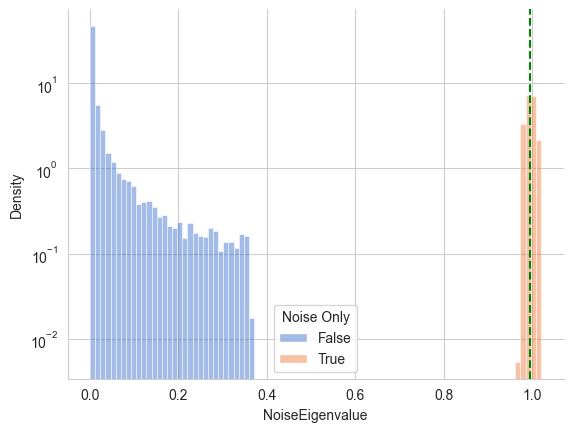
\includegraphics[width=0.45\textwidth]{figures/04_ModelOrderEstimation/noise_eigval_distrib_100k.png}
    \caption{Distribution of noise eigenvalues for \( K = 1e5 \).}
    \label{fig:noise_eigval_distrib_100k}
\end{figure}
Notably, with an increased snapshot count (\( K = 1e5 \)), depicted in \autoref{fig:noise_eigval_distrib_100k}, the
central tendency of the noise eigenvalues for \( N = 0 \) shifts closer to \( \sigma^2_\eta \) which is
in line with expectations. However, the separation between the two clusters—one corresponding to the noise-only case and
the other where signals are present— cannot be explained by the theoretical expectations. \\
Considering that this behavior is consistent across independent simulation environments, it is reasonable to assume that
this bifurcation cannot be explained by a simple ``bug'' in either simulation environment.\\

\subsubsection{Influence of the Model Order}
The emergence of negative eigenvalues within sub-sampled covariance matrices exhibits a strong correlation with the
true model order \( N \). As the complexity of the underlying model increases, the fidelity of the estimated sub-sampled covariance matrix
\( \Csub \) to the true covariance matrix \( \bfm{C}_x \) deteriorates \(\sim\: N \uparrow\; \rightarrow \; \mathcal{L}(\bfm{C}_x, \Csub) \uparrow \).\\
This deterioration is manifested through an increased likelihood of \( \Csub \) losing its positive semi-definiteness.

\begin{figure}[H]
    \centering
    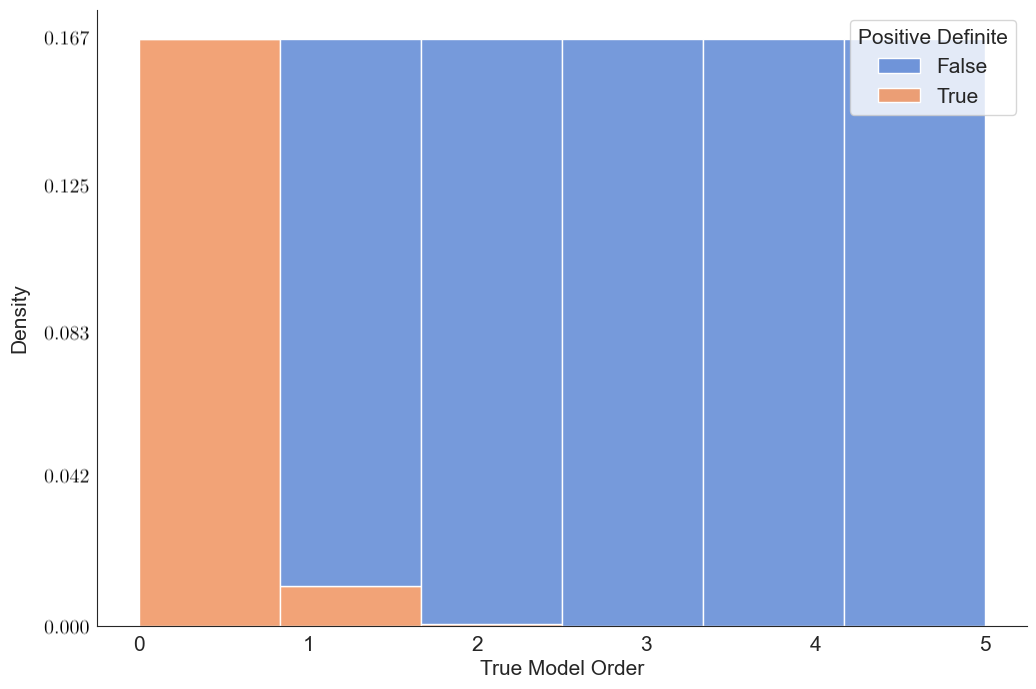
\includegraphics[width=0.45\textwidth]{figures/04_ModelOrderEstimation/eigval_PD_N.png}
    \caption{Illustration of the declining positive definiteness with increasing model order \( N \).}
    \label{fig:eigval_pd_n}
\end{figure}

\autoref{fig:eigval_pd_n}%
\footnote{The data depicted in \autoref{fig:eigval_pd_n} originates from the dataset \( \DMain_{(\text{test})} \), which is discussed in~\autoref{ch:dataset_generation}.}
demonstrates that, at \( K = 100 \), a considerable majority of samples with \( N > 0 \)
experience a loss of positive semi-definiteness in the sub-sampled covariance matrix. \\
Nonetheless, as detailed in~\autoref{ch:evaluation_results}, obtaining reliable model order estimates remains feasible
using the \gls{aic} and \gls{mdl} criteria for most samples where the model order \( N \) is less than the number of RF chains (\( N < L = 3 \)). Furthermore, both the \gls{eft} and deep learning models have been shown to provide accurate model order estimates for \( N \leq 3 \). Empirical evidence indicates that
the eigenvalues retain the ability to encapsulate essential information, enabling accurate predictions of \( N \) even when \( N > 3 \).


\begin{figure}[H]
    \centering
    \subfloat[]{{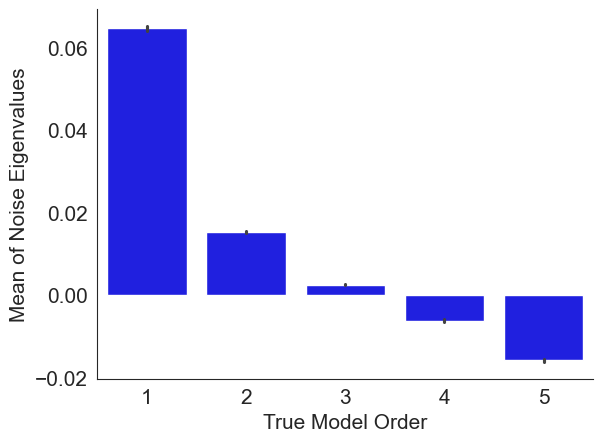
\includegraphics[width=0.37\textwidth]{
        figures/04_ModelOrderEstimation/noise_mean_N.png
    }}}
    \subfloat[]{{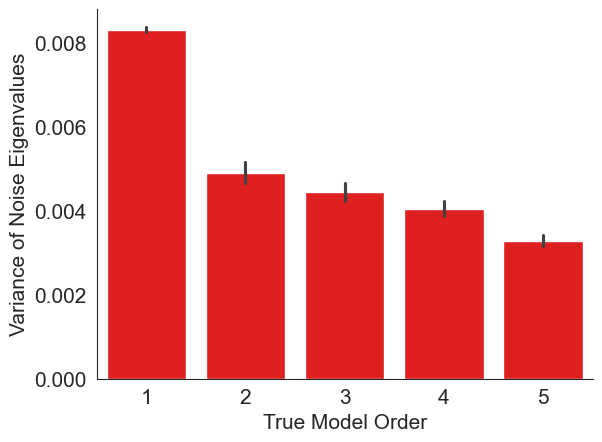
\includegraphics[width=0.37\textwidth]{
        figures/04_ModelOrderEstimation/noise_var_N.png
        }}}
    \caption{
        Mean (a) and variance (b) of the noise eigenvalues for varying model orders \( N \).
    }
    \label{fig:noise_eigval_mean_var_vs_N}
\end{figure}

\autoref{fig:noise_eigval_mean_var_vs_N} illustrates the mean and variance of the noise eigenvalues for varying model orders \( N \).
For sake of interpretability of the linearly scaled y-axis, the mean of the noise eigenvalues for \( N = 0 \) has been omitted from
the plot. \\
The clear correlation between the model order \( N \) and the mean and variance of the noise eigenvalues, can be interpreted
as evidence that the sought-after information about the model order is still encoded within the eigenstructure of the sub-sampled
covariance matrix. Another positive observation is that the \( 95\% \) confidence intervals of mean, as well as the variances
are approximately an order of magnitude smaller than the mean values.

\subsubsection{Influence of the SNR and Number of Snapshots}

Considering that positive definiteness of the covariance matrix seems only to occur for \( N \leq 1 \) for \( K = 100 \),
an evaluation of the relationship between the \gls{sir} and the probability of encountering negative eigenvalues
does not seem to be particularly insightful.\\
However, since both the \( \SNRmin \) and \( \SNRmax \) can already be defined for \( N = 1 \), it appears worthwhile to
investigate the influence of the \gls{snr} on the occurrence of negative eigenvalues.

\begin{figure}[H]
    \centering
    \subfloat[]{{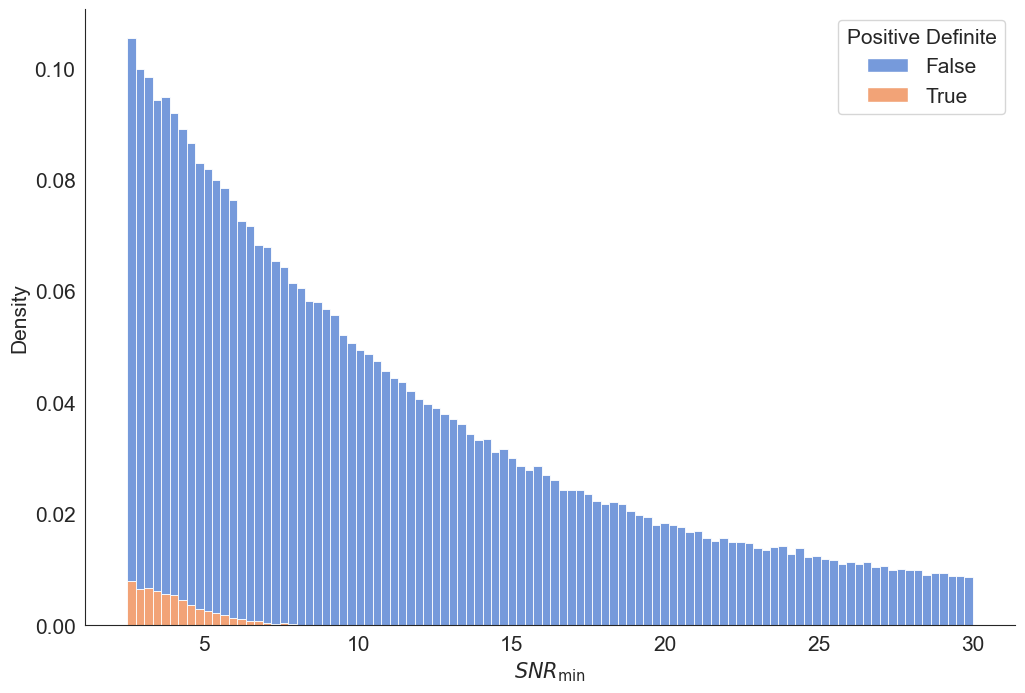
\includegraphics[width=0.33\textwidth]{figures/04_ModelOrderEstimation/snr_hist/min_PD.png}}}
    % \hspace{0.5cm}
    \subfloat[]{{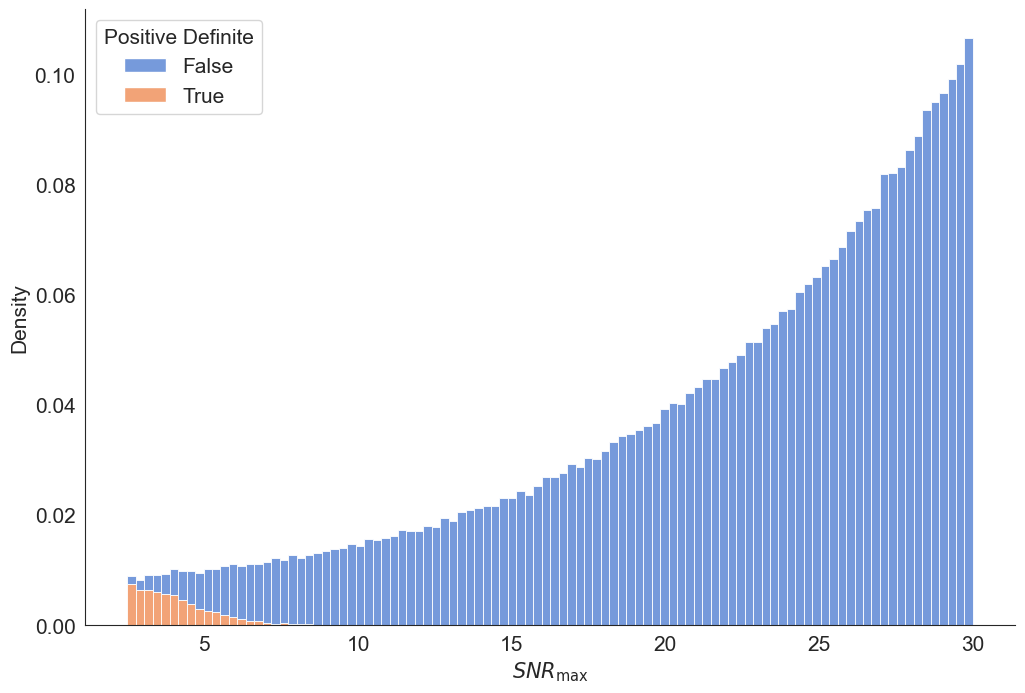
\includegraphics[width=0.33\textwidth]{figures/04_ModelOrderEstimation/snr_hist/max_PD.png}}}
    \caption{Histograms of the \( \SNRmin \) (a), \( \SNRmax \) (b), differentiated w.r.t.\ the positive definiteness.}
    \label{fig:snr_sir_hist}
\end{figure}

\autoref{fig:snr_sir_hist} illustrates the histograms of the \( \SNRmin \) and \( \SNRmax \) values, differentiated with
respect to the positive definiteness of the sub-sampled covariance matrix. \\
As elucidated in the previous chapter, the \gls{pdf} of the \gls{snr} is expected to be a uniform distribution. Utilizing
this knowledge to interpret the histograms, it is evident, that \( \Csub \) quickly loses its positive semi-definiteness
for increasing \( \SNRmin \) and \( \SNRmax \) values.\\


Further insights into the occurrence of negative eigenvalues can be gained by investigating the influence of the number of
snapshots \( K \). Our theoretical expectation is that the sub-sampled covariance matrix should converge asymptotically to the true covariance
matrix -- \( \Csub \rightarrow \bfm{C}_x \) as \( K \rightarrow \infty \). \\
We will therefore investigate the probability of encountering negative eigenvalues for varying numbers of snapshots \( K \)
on the dataset \( \DKvar \) for \( 1 \leq K \leq 1000 \). Subsequently, we will include the \gls{snr} into this evaluation
and present a two-dimensional analysis of the occurrence of negative eigenvalues.

\begin{figure}[H]
    \centering
    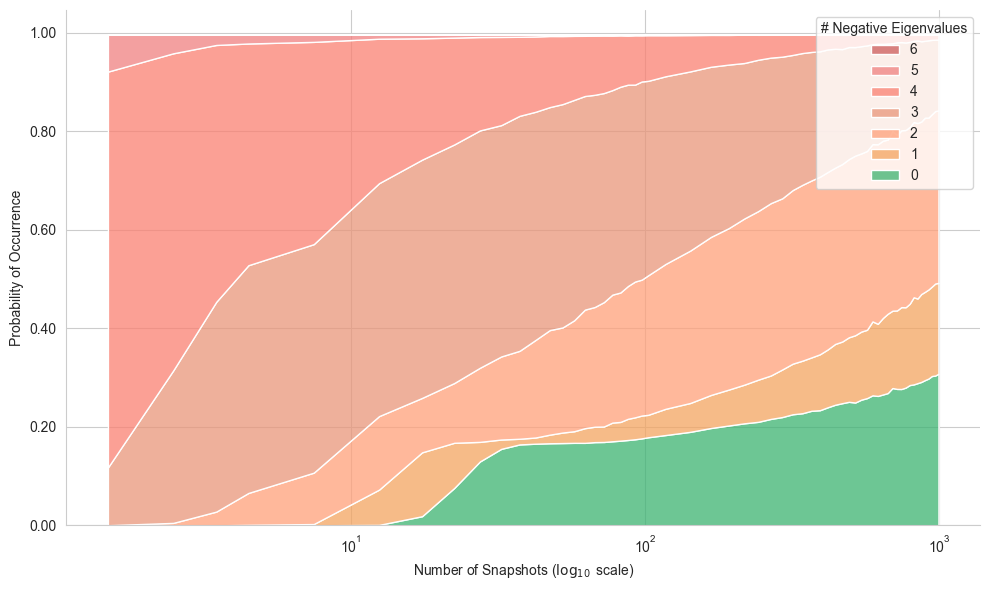
\includegraphics[width=0.8\textwidth]{figures/04_ModelOrderEstimation/num_neg_eigvals_vs_K.png}
    \caption{Probability of encountering \( \ell_{\textit{neg}} \) negative eigenvalues for varying numbers of snapshots \( K \).}
    \label{fig:num_neg_eigvals_vs_K}
\end{figure}

\autoref{fig:num_neg_eigvals_vs_K} illustrates that the likelihood of \( \Csub \) being positive semi-definite asymptotically
increases with \( K \), aligning with theoretical insights presented in~\cite{meyer}.
According to the observations, depicted in~\autoref{fig:eigval_pd_n}, the probability of encountering negative eigenvalues
at \( K = 100 \) should be approximately
\[
    \Pr(\ell_{\textit{neg}} > 0|K=100) = 1 - \Pr(\ell_{\textit{neg}} = 0| K=100) \approx  1 - (0.1\overline{6} + 0.01) = 0.82\overline{3}.
\]

Given the close agreement between both%
\footnote{\autoref{fig:eigval_pd_n} being observed on \( \DMain_{(\text{test})} \) and \autoref{fig:num_neg_eigvals_vs_K} on \( \DKvar \) for \(K = 100\).}
observed probabilities, we are poised to continue with the two-dimensional analysis.



\begin{figure}[H]
    \centering
    \subfloat[]{{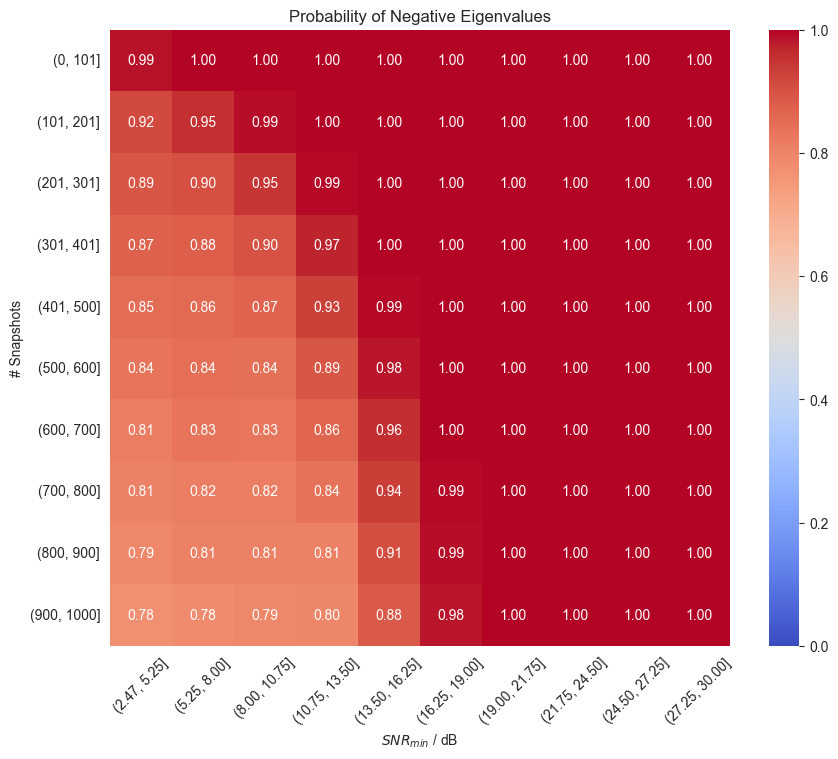
\includegraphics[width=0.45\textwidth]{figures/04_ModelOrderEstimation/snr_min.png}}}
    % \hspace{0.5cm}
    \subfloat[]{{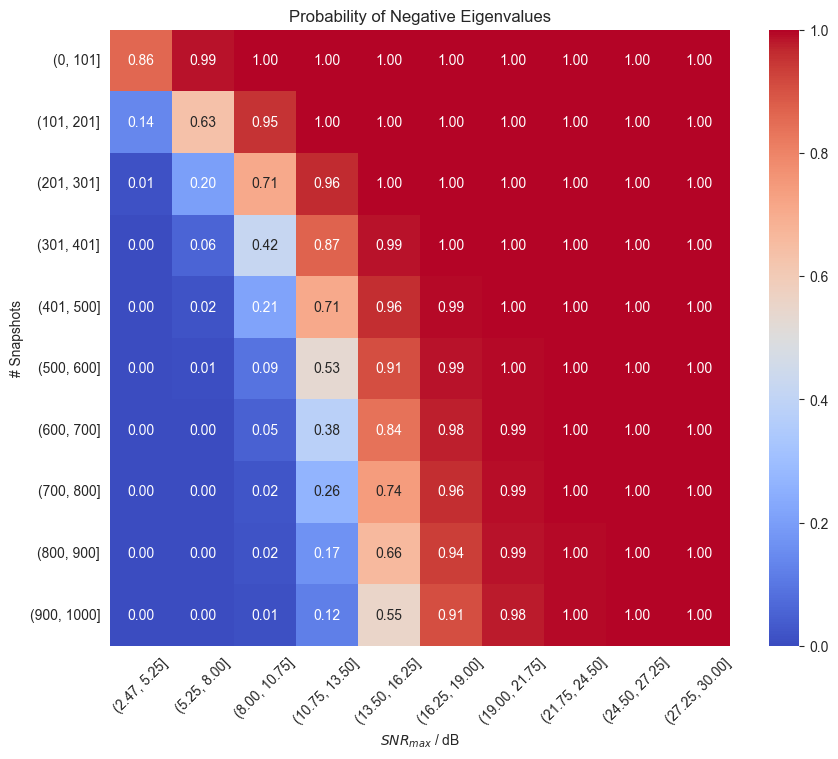
\includegraphics[width=0.45\textwidth]{figures/04_ModelOrderEstimation/snr_max.png}}}
    \caption{Probabilities of negative eigenvalues for the minimum (a) and maximum (b) \gls{snr}, for a varying number
    of snapshots.}
    \label{fig:snr_num_snapshots_pd}
\end{figure}

\autoref{fig:snr_num_snapshots_pd} shows that high \( \SNRmin \) and \( \SNRmax \) values strongly correlated with a
higher probability of negative eigenvalues. Whereas the \( \Pr(\ell_{\textit{neg}} > 0) \) seems to be mostly dependent
on \( N \) for \( K = 100 \), it is evident that other even hg


\subsubsection{Handling Negative Eigenvalues}
To still be able to use the beforementioned algorithmic methods, the eigenvalues need to be transformed so that the resulting
vector \( \bfL \) only contains non-negative values.
Since the \gls{aic}, \gls{mdl}, and \gls{eft} cannot cope with non-positive eigenvalues, they had to be inferred from transformed
eigenvalues \( \widetilde{\bfL} \) whose positivity was ensured according to~\autoref{eq:pos_eigvals}.

\begin{align}
    \widetilde{\bfm{\lambda}} &=
    \begin{cases}
      \bfm{\lambda} + \lambda_M + \epsilon_{\text{eft}} & \text{if } \lambda_M \leq \epsilon_{\text{eft}} \text{ for \gls{eft}}, \quad \epsilon_{\text{eft}} = \num{1e-6} \\
      \bfm{\lambda} + \lambda_M + \epsilon_{\text{IC}} & \text{if } \lambda_M \leq \epsilon_{\text{IC}} \text{ for \gls{aic} and \gls{mdl}}, \quad \epsilon_{\text{IC}} = \num{1} \\
      \bfm{\lambda} & \text{otherwise}
    \end{cases}
    \label{eq:pos_eigvals}
\end{align}

The additional offset term \( \epsilon_{\text{IC}} \) was introduced to ensure that \( \widetilde{\bfm{\lambda}}_{\text{IC}} \)
does not contain any values close to zero, which would result in most criteria values \( \bfm{\mathrm{AIC}}[n] \)  and \( \bfm{\mathrm{MDL}}[n] \) diverging to
\( \infty \). Lower values of \( \epsilon_{\text{IC}} \) appear to be correlated with a higher bias. A value of \( \epsilon_{\text{IC}} = 1 \) was chosen,
since \( \sigma^2_{\eta} = 1 \), and therefore the noise eigenvalues \( \bfm{\lambda}_{\eta} \) are expected to cluster around 1.\\
\gls{mdl} exhibited a slightly better performance in terms of bias and variance for eigenvalues \( \widetilde{\bfL} \) being
transformed by
\begin{equation}
    \mathcal{TF} \coloneq \{\| \bullet \| \rightarrow \text{sort}(\bullet) \rightarrow \bullet = \bullet + \epsilon_{\text{IC}}\}, \quad \mathcal{TF} : \bfL \mapsto \widetilde{\bfL}.
\end{equation}
The \gls{eft}, conversely, only requires a small offset to ensure that the eigenvalues are greater than zero. Increasing
the offset reduces the goodness of fit of the \gls{eft}'s predicted eigenvalue profile to the true eigenvalues.

% \section{Factors Influencing \gls{moe}}
% The \gls{moe} methods discussed in this thesis depend on the distribution of eigenvalues. Important factors influencing \gls{moe}
% include the \glsfirst{snr}, \glsfirst{sir}, the array's aperture \( D \), finite-sample effects when \( K < 10M \),
% modeling errors, and the impact of sub-sampling. As the conventional methods used at Rohde \& Schwarz are affected by
% these factors, they will be discussed further at the end of this chapter~\cite{meyer}.\\


% - multipath -> rank deficient -> overfitting -> higher model order: `By partitioning the whole array into sub-
% arrays and averaging of the sub-array received covariance matrices, the equivalent source covariance matrix becomes
% nonsingular. The FBSS scheme is widely-used since it can be regarded as a preprocessing before applying AIC and MDL [9]
% as well as DOA estimation algorithms`'\cite{yang2020}

% ---

% \begin{align}
%     \mathcal{H}_{p+1} &: \lambda_{M-p} \in \bfL_\eta \label{eq:hypothesis_noise} \\
%     \widetilde{\mathcal{H}}_{p+1} &: \lambda_{M-p} \in \bfL_S \label{eq:hypothesis_signal}
% \end{align}

% Starting with the pair \( (\lambda_{M-1}, \hat{\lambda}_{M-1}) \), the relative distance between each of the
% theoretical noise eigenvalues and their corresponding observed eigenvalue is computed. This difference is then assessed
% against a predefined threshold value \( \tau_n \), which scales with the eigenvalue index. The condition for
% determining the hypothesis to accept is as follows:

% \begin{equation*}
%     \lambda \in \left\{
%         \begin{array}{ll}
%             \bfL_{\eta}, & \text{if } \left|\frac{\lambda_{M-p} - \hat{\lambda}_{M-p}}{\hat{\lambda}_{M-p}}\right| = \epsilon_n \leq \tau_n, \\
%             \bfL_{S}, & \text{otherwise}.
%         \end{array}
%     \right.
% \end{equation*}
% \input{chapters/05_ModelOrderEstimationDL.tex}
\chapter{Model Exploration}
\label{ch:model_exploration}

\section{Introduction}

This chapter aims to outline the exploration of the inspected model and hyperparameter space.
The selection of the most appropriate form of input data forms the cornerstone of this exploratory process.
Subsequently, the chapter delves into the potential preprocessing steps that can be applied to the input data to increase
its suitability as input to \glspl{dnn}.\\
The chapter then extends to the architectural design choices of the models. The considered architectures are
variations of the classical dense, convolutional, and recurrent neural networks.
The \gls{cnn} and \gls{rnn} based models will be explored in more detail than the \gls{mlp} architecture, as they provide
each provide unique advantages for the task at hand, whereas the \gls{mlp} mostly serves as a baseline model.\\
A comparative analysis of the different model architectures among themselves and with the previously introduced algorithms
will then be conducted in~\autoref{ch:evaluation_results}.

\section{Choice of Input Data}

Selecting the optimal form of input data is a paramount initial step in designing \glspl{dnn}.
This choice is influenced by the data's capacity to efficiently encode the coveted information, ensuring that the model
can effectively learn and generalize from the input data, without overfitting on irrelevant features.


\subsection{Evaluation of Input Data Forms}

Various forms of input data were considered, assessing their potential in effectively conveying information pertinent to
model order estimation:

\textbf{Measurement Matrix \( \bfm{X} \):}
The sub-sampled measurement matrix \( \bfm{X} \in \mathbb{R}^{M \times L} \) contains the IQ samples of the
individual subarrays, each column consisting of \( L \) complex data points. \\
This form of input data offers a direct signal representation but entails the highest dispersion of the sought-after
model order information.

A system with \( M = 9 \) antennas, \( L = 3 \) RF chains, and \( K = 100 \) snapshots would result in a matrix with
\begin{equation}
    \#\text{Elements} = 2 \cdot K \cdot J \cdot L = 7200 \text{ samples.}
\end{equation}
As per~\autoref{subsec:IncoherentMeasurementVector}, \( J \) denotes the number of subarrays, and the factor of two
accounts for the real and imaginary parts of the complex samples. It is evident that a potential model would need to be able
to handle a varying number of samples, which would be a significant downside of this form of input data.

Contrasting to the downside of the low information density, it is clear that
the measurement matrix \( \bfm{X} \) contains uncorrupted information about the model order \( N \). However, it would
require a much more sophisticated and complex model to extract this information and would have a higher risk of overfitting%
\footnote{This would be especially problematic given probable discrepancies between synthetic and real-world data.}.
This form of input data can thus be considered most unsuitable for the task at hand.

\textbf{Eigenvectors \( \bfm{U} \):}
Eigenvectors derived from the covariance matrix are fundamentally scale-invariant,
making them unsuitable for discerning the model order \(N\) directly. This scale-invariance implies that multiplying an
eigenvector by any scalar does not affect its direction or its role in spanning the signal or noise subspaces~\cite{axler.ch5}.
This claim is an obvious consequence of the definition of eigenvectors, as shown in \autoref{eq:eigenvector_definition}.
\begin{equation}
    \bfm{U} = \left\{ \nu \bfm{u}_i \,\middle|\, \bfm{u}_i \in \mathbb{R}^M \land \bfm{C}\bfm{u}_i = \lambda_i\bfm{u}_i,\: \nu \in \mathbb{R} \right\}
    \label{eq:eigenvector_definition}
\end{equation}

Moreover, the orthogonal relationship between the noise subspace and the signal subspace further diminishes the utility of eigenvectors as potential input data.
Since \( \bfm{U}_\eta \perp \bfm{U}_S \), the directional properties of the eigenvectors do not encode information
pertinent to the model order \(N\).

\textbf{Covariance Matrix \( \bfm{C} \):}
A logical consequence of the eigenvector's unsuitability is that the covariance matrix cannot hold any additional information
about the model order \( N \) beyond what is encapsulated in the eigenvalues. Although, this conclusion can already be drawn
from \autoref{eq:eigenvector_definition}, it might be helpful to reiterate that the covariance matrix is simply a linear
combination of the eigenvectors and eigenvalues, as shown in \autoref{eq:covariance_matrix_eigenvalue_decomposition}.
\begin{equation}
    \bfm{C}_x = \bfm{U}_S \bfm{\Lambda}_S \bfm{U}_S^H + \bfm{U}_{\eta} \bfm{\Lambda}_{\eta} \bfm{U}_{\eta}^H
    \label{eq:covariance_matrix_eigenvalue_decomposition}
\end{equation}

Despite recent studies~\cite{barthelme21sub, yu22RCNN, barthelme2020} demonstrating the efficacy of covariance matrix-based deep learning models,
we decided against pursuing this approach, based on unsatisfactory results from internal research, that tried to replicate the
findings in~\cite{barthelme2020}.
While the replication yielded promising results for low \gls{sir}, the performance of the model dropped below the performances
of the classical \gls{aic} and \gls{mdl} for higher \gls{sir} values. \\

\textbf{Eigenvalues \( \bfL \):}
The previous considerations lead to the conclusion that the eigenvalues of the covariance matrix are the most suitable
choice for input data. The distribution and magnitude of the \( M \) eigenvalues in \( \bfL \) must encapsulate the model
order \( N \) in the most effective manner. This decision as well as the reasoning are in line with the findings in~\cite{yang2020}.\\
A practical downside of using eigenvalues as input data is the exorbitant computational cost of the eigenspace decomposition.
Though, given the pre-existing necessity of this operation, as a preliminary step for the employed super-resolution algorithms, the
eigenvalues-as well as all other discussed alternatives-are already available in the computational pipeline of the considered
direction finding systems.\\
Nonetheless, the degradation of the information encoded into the eigenvalues due to the loss of positive semi-definiteness
in the covariance matrix remains an unresolved topic of concern. This issue is subject to further investigation
in~\autoref{ch:evaluation_results}.


\section{Input Data Preprocessing}
\label{sec:input_data_preprocessing}

\subsubsection{Transposition of Eigenvalues}
% TODO add formulas on transponation of the vector of eigenvalues to either (B, 1, M), (B, M, 1) or (B, M),
Different types of \glspl{dnn} necessitate specific tensor shapes for their input data. Hence, a transposition of the vector of
eigenvalues \( \bfL \in \mathbb{R}^M \) is imperative. The batch size \( \B \) adds a dimension during training, which
must be accounted for in the input tensor.

\begin{align}
    &\bullet \; \textbf{Fully Connected Layers:} & (\B, \#\textit{features}) \;& \longleftrightarrow \; T_{\mathrm{FC}} : \bfL \mapsto \bfLT_{\mathrm{FC}} \in \mathbb{R}^{\B \times M} \label{eq:transposition_mlp}\\
    &\bullet \; \textbf{Convolutional Layers:} & (\B, \#\textit{channels}, L) \;& \longleftrightarrow \; T_{\mathrm{CNN}} : \bfL \mapsto \bfLT_{\mathrm{CNN}} \in \mathbb{R}^{\B \times 1 \times M} \label{eq:transposition_cnn}\\
    &\bullet \; \textbf{Recurrent Layers:} & (\B, L, \#\textit{features}) \;& \longleftrightarrow \; T_{\mathrm{RNN}} : \bfL \mapsto \bfLT_{\mathrm{RNN}} \in \mathbb{R}^{\B \times M \times 1} \label{eq:transposition_rnn}
\end{align}

The \( L \) in the equations~\ref{eq:transposition_cnn} and~\ref{eq:transposition_rnn} denote the length of the \gls{cnn}'s and
\gls{rnn}'s input ``sequence''.
\( T_{\mathrm{FC}} \), \( T_{\mathrm{CNN}} \), and \( T_{\mathrm{RNN}} \) are the transposition functions for the respective layer types, and
\( \bfLT_{\mathrm{FC}} \), \( \bfLT_{\mathrm{CNN}} \), and \( \bfLT_{\mathrm{RNN}} \) are the transposed input tensors.\\
To allow a more intuitive understanding of the resulting tensor shapes, we will briefly describe how the employed layer
types will ``perceive'' their respective input data for the unbatched case.
Whereas the fully connected layers expect a one dimensional input tensor, whose \( M \) elements are considered
spatially independent individual features, the convolutional layers regard the input as single-channel one-dimensional
signals, whose singular spatial dimension consists of \( M \) elements.
The recurrent layers, on the other hand, regard the input as a temporal sequence whose length \( L \) equals the number
of eigenvalues \( M \), with each element of the sequence being a singleton feature.

To facilitate an intuitive grasp of how the data is structured post-transposition, and how slices of the tensors are
retrieved for analysis or further processing, the following notations will be adopted:
\begin{align*}
    &\bfLT := \bfLT_{\mathrm{FC}} \\
    &\bfLT^{\D} := \textit{Tensor of entire dataset } \D \\
    &\bfLT^{\D}_{:,i} := \textit{Slice through } \bfLT^{\D} \textit{, selecting the i-th column} \\
    &\overline{\bfLT}_{:, :} := \textit{Mean of all samples in } \D \\
    &\bfLT^{\D}_{:,:N}:= \textit{Signal eigenvalues across all samples in } \D
\end{align*}


\subsubsection{Input Data Normalization}
\label{subsec:input_data_normalization}

Normalization is a commonly utilized preprocessing step in deep learning, enhancing the model's training efficiency and numerical
stability. While theoretically, neural networks can learn to adjust scaling factors autonomously,
input normalization aids in the rapid convergence of initial layers by ensuring uniformity in the scale of input features,
which is particularly beneficial in avoiding potential issues with biased gradients and enabling higher learning rates by
mitigating ``zigzag''-like trajectories through the loss landscape~\cite{yangMedium2020}.

Typically, normalization in \glspl{cnn} and \glspl{rnn} is applied across channels-or features-, ensuring that the mean and
the standard deviation of each feature are \( \mu_{\bfm{x}_{\mathrm{ch},:}} = 0 \) and \( \sigma_{\bfm{x}_{\mathrm{ch},:}} = 1 \).\\
Given our data's structure (Equations \ref{eq:transposition_mlp} \( \ldots \) \ref{eq:transposition_rnn}), normalization could be applied
either channel-wise over all samples in the dataset-which would align with the typical approach for \glspl{cnn}-, sample-wise
where each vector of eigenvalues is normalized independently of the dataset, or index-wise, normalizing along the spatial
indices of the eigenvalues.\\
The latter approach seemed most suitable at the time of implementation, as it respects the spatial nature of the eigenvalues,
ensuring that each eigenvalue's contribution is scaled uniformly, and is formulated as follows:

\begin{algorithm}[H]
    \caption{Index-wise Normalization of Eigenvalues}
    \label{alg:index_wise_normalization}
    \DontPrintSemicolon
    \KwIn{\;
        \quad \( \DTrain \): Training split of \( \DMain \)\;
    }
    \KwOut{\;
        \quad \( \widetilde{\bfLT} \): Tensor of normalized eigenvalues
    }

    \SetKwFunction{FMain}{IndexWiseNormalize}
    \SetKwProg{Fn}{Function}{:}{}
    \Fn{\FMain{\(\DTrain\)}}{
        \(\bfLT \gets T_{\mathrm{FC}}(\DTrain.\mathrm{Eigenvalues})\)\;
        \(\widetilde{\bfLT} \gets\) empty tensor of shape \(\bfLT.\mathrm{Shape}\)\;
        \For{\(i \gets 0\) \KwTo \(M-1\)}{
            \( \mu_i \gets \mathbb{E}[\bfLT_{:,i}] = \frac{1}{\B} \sum_{b=1}^{\B} \bfLT_{b,i} \)\;
            \( \sigma_i \gets \sqrt{\mathbb{E}[(\bfLT_{:,i} - \mu_i)^2]} = \sqrt{\frac{1}{\B} \sum_{b=1}^{\B} (\bfLT_{b,i} - \mu_i)^2} \)\;
            \For{\(b \gets 1\) \KwTo \(\B\)}{
                \( \widetilde{\bfLT}_{b,i} \gets \frac{\bfLT_{b,i} - \mu_i}{\sigma_i} \)\;
            }
        }
        \KwRet \( \widetilde{\bfLT} \)\;
    }
\end{algorithm}

The impact of the index-wise normalization on the distribution of the eigenvalues is depicted in \autoref{fig:eigenvalues_norm},
showcasing violin plots for each eigenvalue index both before and after normalization.

\begin{figure}[H]
    \centering
    \subfloat[]{{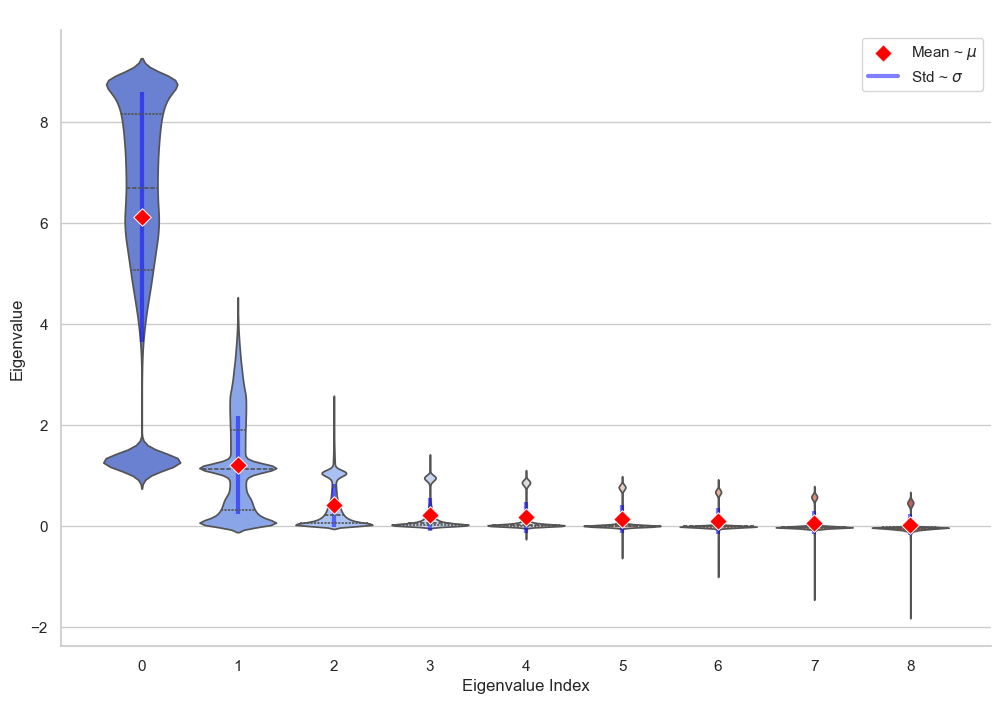
\includegraphics[width=0.5\textwidth]{figures/06_ModelExploration/1_InputData/eigval_violin_raw.png}}}
    \subfloat[]{{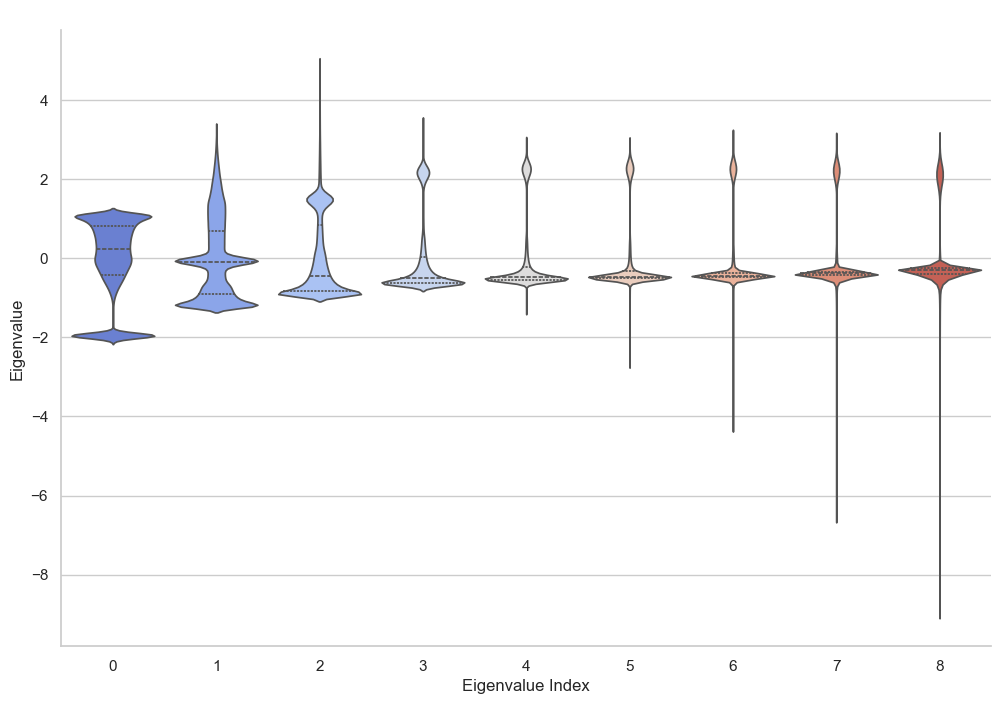
\includegraphics[width=0.5\textwidth]{figures/06_ModelExploration/1_InputData/eigval_violin_norm.png}}}
    \caption{Distributions of the eigenvalues \( \bfL \) before (a) and after (b) index-wise normalization.}
    \label{fig:eigenvalues_norm}
\end{figure}

The violin plot of the unnormalized
eigenvalues, shows that the eigenvalues, belonging noise-only scenarios, are clustered around the noise variance \( \sigma^2_{\eta} = 1\si{\micro\volt\squared}\),
and that an intuitive manual separation of the signal and noise eigenvalues is in most cases only possible for \( N < 3 \).
\hyperref[fig:eigenvalues_norm]{Figure~\ref*{fig:eigenvalues_norm}a} also depicts the mean and standard deviation of the
unnormalized eigenvalues, which additionally are gathered in \autoref{tab:dataset_stats}.

\begin{table}[H]
    \centering
    \caption{Statistics of Training Dataset Eigenvalues}
    \label{tab:dataset_stats}
    \begin{tabular}{lrrrrrrrrr}
    \toprule
    & \multicolumn{9}{c}{\textbf{Eigenvalue Index}} \\
    \cmidrule{2-10}
    & 1 & 2 & 3 & 4 & 5 & 6 & 7 & 8 & 9 \\
    \midrule
    \( \mu_i \) & 6.122 & 1.220 & 0.419 & 0.236 & 0.179 & 0.143 & 0.110 & 0.075 & 0.035 \\
    \( \sigma_i \) & 2.478 & 0.973 & 0.428 & 0.334 & 0.305 & 0.279 & 0.253 & 0.229 & 0.203 \\
    \bottomrule
    \end{tabular}
\end{table}



The evaluation of index-wise normalization's role in enhancing the predictive capabilities of an early \gls{cnn} iteration,
is detailed in \autoref{tab:model_performance}.

\begin{table}[H]
    \centering
    \caption{Impact of input data normalization on model performance}
    \label{tab:model_performance}
    \begin{tabular}{@{}lcccccc@{}}
    \toprule
    & \multicolumn{2}{c}{\( \meanLossCEVal \)} & \multicolumn{2}{c}{ \( \meanAccVal \)} & \multicolumn{2}{c}{\#MACs} \\
    \cmidrule(lr){2-3} \cmidrule(lr){4-5} \cmidrule(lr){6-7}
    Normalization & \( \nu \) & \( \%\Delta \) & \( \nu \) & \( \%\Delta \) &  &\\
    \midrule
    False & 0.616 & — & 0.725 & — &  — \\
    True & 0.615 & \gnbx{-0.30\%} & 0.726 & \gnbx{0.06\%} & \redbigoplus{} \\
    \bottomrule
    \end{tabular}
\end{table}

The results in \autoref{tab:model_performance} indicate that the index-wise normalization yields only a marginal improvement in the
model's performance, with a slight decrease in the mean validation loss%
\footnote{
    \( \meanLossVal \coloneq \mathbb{E}_{(\mbf{Z}, \mbf{Y}_N) \sim \DVal}[\lossCEVal(\mbf{Z}, \dot{\mbf{Y}}_N)]\), \( \mbf{Z} \) being
    the model's logits, and \( \dot{\mbf{Y}}_N \) the one-hot encoded ground truth labels.
}.
and a neglectable increase in the validation accuracy,
while coming at the cost of an increased number of \glspl{mac} through the additional normalization operations.


\subsubsection{Reevaluation of Index-wise Normalization}
\label{subsubsec:reevaluation_index_wise_normalization}

Upon retrospective reflection of the index-wise normalization approach, several insights have emerged that warrant
reconsideration of its appropriateness for the task at hand.

Firstly, the examination of the eigenvalue distribution underscores a relatively constrained variance, particularly
highlighted by a manageable peak to peak spread and level difference:
\begin{align*}
    \Delta\lambda_{pp} &= \max(\bfLT^{\D}_{:,:}) - \min(\bfLT^{\D}_{:,:}) \approx 11.2\si{\micro\volt\squared}, \\
    L_{\mu,pp} &= L_{\mu_1} - L_{\mu_M} = \num{44.9}\si{\decibel}.
\end{align*}

The practice of index-wise normalization, while theoretically enhancing uniformity across eigenvalue magnitudes,
amplifies the variability of lower-magnitude eigenvalues due to their low relatively low standard deviation and the
resulting inherent reciprocal scaling effect on outliers. This increased spread would mostly affect noise eigenvalues,
whose values might not encode any meaningful information about the model order, due to the effects of sub-sampling.
Enforcing uniformity across the priorities of all eigenvalues might not be aligned with the task's inherent
requirements.

Another argument advocating against normalization is the fact that the mean and standard deviation of some eigenvalues
exhibit low absolute values, which would exacerbate numerical errors in low-precision computational environments.
The subtraction of two relatively small numbers and the subsequent division by a small number would most likely lead to
the occurrence of high numerical errors, especially in the case of hardware implementation, which would require lower
precision fixed-point numbers.

Given the neglectable performance gain and the additional computational cost, the low complexity of the input data, and
the aforementioned detrimental effects, it was decided not to utilize the normalized eigenvalues as input data for the
networks.



% \section{Previous Deep Learning Approaches}
% [\cite{yang2020}]
% ```
% Based on information theory [6], the covariance matrix C contains the key information for the source number detection. One natural idea is to employ DNN to learn the source number directly from the covariance matrix C. However, it is would not be an effective way to to so due to the information redun- dancy in C that contains all unknown information besides the number of sources (will be verified in simulations).
% Although DL exhibits powerful learning capability in extracting features from massive data, model information, if can be well utilized, would provide significant enhancement in performance [11]. To see this, let us express C as

% where lambda and um are the m-th eigenvalue and correspond- ing eigenvector of C, respectively. From the array signal processing theory [5], the eigenvectors would construct the signal subspace and the noise subspace, from which the ESPRIT and MUSIC algorithms can be applied to estimate the DOA, respectively. Nevertheless, it is clearly that eigenvectors themselves do not contain information of the number of the sources and hence would bring redundancy if being input to the DNN. Hence, instead of input the whole C, we propose to only input the DNN the eigenvalues , which is also consistent with the AIC and MDL approaches. Notice that the eigenvalues  are all real numbers, therefore, complex operations are not required in the proposed ERNet and ECNet.
% ```
% They employed a fully connected NN, and no sub-sampling
% + Eigenvalues and Eigenvectors are \( \in \mathbb{R} \) and not complex such as the covariance matrix
% + \cite{yang2020} showed <überlegene> performance of eigenvalues over covariance matrix in for non-coherent sources and varying numbers of snapshots
% - \cite{yang2020} When the sources are coherent, which is the common in the real environment, the signal covariance matrix is rank- deficient, and therefore the performance of eigenvalue based methods degrades [16]. To solve the problem, the FBSS scheme is adopted [9], where the the total array of M antennas is divided forward/backward into overlapping sub-arrays with size M 0. The number of forward/backward sub-arrays is T = M - M0 + 1. Note that the M0 >     K and T >= K should be satisfied as proved in [16]. Then, the forward/backward averaged covariance matrix is given by [9]


\section{Choice of Optimization Objective}

\subsection{Regression}
When faced with the challenge of estimating discrete ordinal quantities, such as the number of sources in model order estimation tasks,
the initial inclination might lean towards employing regression models.
At first glance, these models offer a straightforward approach, potentially allowing for the interpretation of their
quasi-continuous output as a discrete source count after appropriate rounding.\\
However, this method exhibits intrinsic limitations due to the absence of inherent output bounds in regression models,
leading to the necessity for artificial scaling interventions.

Solutions like applying a scaled sigmoid function to the regression layer's output have been contemplated to confine the
predictions within the required range of \( [0, N_{\max}] \).\\
Despite its theoretical viability, this approach inadvertently biases the model towards mid-range values,
complicating the differentiation between adjacent classes, especially at the boundary values.

A more feasible alternative is to transform the output of the regression layer according, would be to round it to
the nearest integer and clamp it, such that it falls within the valid range of source counts.
% Add a brief explanation of ˜\hat{bfm{y}}_reg˜ - single neuron output -> #Params in regression layer: # CHs_prev_layer * 1
\begin{equation}
    \bfm{\NPred}_{\text{reg}} = \max\left(0,\:\min(N_{\max},\:\nint{\hat{\bfm{y}}})\right), \quad \hat{\bfm{y}} \in \mathbb{R}^{\B}, \: \bfm{\NPred}_{\text{reg}} \in \NSet^{\B}
    \label{eq:regression_clamp}
\end{equation}

Similarly to~\cite{yang2020} we decided to employ the \gls{mse} (\( \mathcal{L}_2 \)) loss function for the regression model.
\begin{equation}
    \lossMSE(\hat{\bfm{y}}, \bfm{N}) = \frac{1}{\B} \sum_{i=1}^{\B} \left(\hat{y}_i - N_i\right)^2, \quad \hat{y}_i \in \mathbb{R},\: N_i \in \NSet
    \label{eq:mse_loss}
\end{equation}

\subsection{Classification}
For convenience, let \( C \coloneq N_{\max} + 1 = \| \NSet \| \) denote the number of classes in the classification task.\\
The classification approach provides a more intuitive and efficient solution to the task. Rather than using a regression
layer with a single neuron output, we utilize a classification layer that produces a tensor of logits \( \bfm{Z} \in \mathbb{R}^{\B \times C}\).
This enables the classification model to have separate output units for each class.\\
To denote the logits vector for a specific sample within the batch, let \( \bfm{z} \coloneq \bfm{Z}_{b,:} \),
where \( \bfm{z} \in \mathbb{R}^{C} \) represents the logits for the \( b \)-th sample across all \( C \) classes.\\
The interpretation of each element within the logits vector \( \bfm{z} \) corresponds to the log-likelihood for class
memberships, where \( z_c = \ln \Pr(N=c|\bfL; \bfm{\omega}) \) represents the logarithm of the probability that
the model order \( N \) equals class \( c \), conditioned on the input \( \bfL \) and parameterized by the model weights
\( \bfm{\omega} \)~\cite[Chapter 6]{dlbook}.

During inference, the model order estimate \( \NPred_{\text{cls}} \) is obtained by determining the index of the maximum element in
the logits vector \( \bfm{z} \):
\begin{equation}
    \bfm{\NPred}_{\text{cls}} = \argmax_{c \in \NSet} \bfm{Z}_{:,c}, \quad \bfm{\NPred}_{\text{cls}} \in \NSet^{\B}
    \label{eq:classification_argmax}
\end{equation}

For the purpose of training, however, the softmax activation function is applied to the logits, converting them into a valid probability
distribution across the class labels. The transformation \( \mathrm{softmax} : \mathbb{R}^C \rightarrow [0, 1)^C \) is defined by:
\begin{equation}
    \hat{y}_c = \text{softmax}(\bfm{z})_c = \frac{e^{z_c}}{\sum_{j=1}^{C} e^{z_j}}, \quad c \in \NSet
    \label{eq:softmax}
\end{equation}
where \(\hat{y}_c\) represents the predicted probability that the model assigns to class \(c\), given the logits
vector \(\bfm{z}\) for a specific sample. The softmax function ensures that the output probabilities sum to one,
facilitating a direct comparison with the true class labels.

Consequently, the cross-entropy loss function is utilized to quantify the discrepancy between the predicted probability
distribution and the true label distribution and is defined as follows:
\begin{equation}
    \lossCE(\hat{\bfm{Y}}, \dot{\mbf{Y}}_N) = -\frac{1}{\B} \sum_{b=1}^{\B} \sum_{j=1}^{C} N_{bj} \ln(\hat{y}_{bj}), \quad \dot{\mbf{Y}}_N, \hat{\bfm{Y}} \in \mathbb{R}^{\B \times C}
    \label{eq:ce_loss}
\end{equation}
In \autoref{eq:ce_loss}, \( \dot{\mbf{Y}}_N \) represents the true class labels in one-hot encoding. Each row of \( \hat{\bfm{Y}} \),
denoted as \( \hat{\bfm{y}} = [\hat{y}_1, \ldots, \hat{y}_c] \), represents the model's predicted probabilities for a particular sample.

\subsection{Comparison and Conclusion}

\begin{figure}[H]
    \centering
    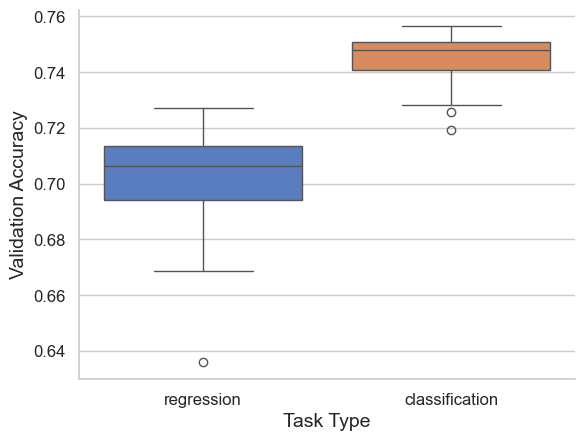
\includegraphics[width=0.45\textwidth]{figures/06_ModelExploration/conv_task_type.png}
    \caption{Boxplot of \( \meanAccVal \) for the regression and classification tasks.}
    \label{fig:task_type}
\end{figure}

Figure~\ref{fig:task_type} compellingly demonstrates the superior performance of the classification paradigm over
regression in terms of validation accuracy. A brief explanation of the employed boxplots is provided in~\autoref{app:sec:Boxplot}.
To quantify this advantage,~\autoref{tab:accuracy_change} details the relative improvement when switching from regression
to classification.

\begin{table}[H]
    \centering
    \caption{Quantitative Performance Metrics: Regression vs. Classification}
    \label{tab:accuracy_change}
    \begin{tabular}{@{}lcc@{}}
    \toprule
    & \multicolumn{2}{c}{\( \meanAccVal \)} \\
    \cmidrule(lr){2-3}
    Task Type & \( \nu \) & \( \%\Delta \) \\
    \midrule
    Regression~\bigoplus~\( \lossMSE \) & 0.7062 & — \\
    Classification~\bigoplus~\( \lossCE \) & 0.7478 & \gnbx{+5.889\%} \\
    \bottomrule
    \end{tabular}
\end{table}

The data presented in \autoref{tab:accuracy_change} as well as the boxplots in \autoref{fig:task_type} were obtained by optimizing for
the respective loss functions \( \lossMSE \) and \( \lossCE \) on the validation set \( \DMain_{(\text{val})} \) using an
earlier the \gls{cnn} architecture, which will be introduced in \autoref{sec:cnn}.


The only downside of employing the classification approach is an increase in computational cost due to the
additional \( C - 1 \) neurons in the output layer. Assuming a total of \( K_{\text{CH}} \) channels or features in the
previous layer, the number of parameters in the output layer for both tasks given by:
\begin{align}
    \#\text{Params}_{\text{head,reg}} &= K_{\text{CH}} \times 1 \\
    \#\text{Params}_{\text{head,cls}} &= K_{\text{CH}} \times C
\end{align}

This increased computational cost is a small price to pay for the significant improvement in performance, which is
why we decided to proceed with the classification approach for the remainder of the study. Both, the softmax activation
function and the multi-class cross-entropy loss function are embedded into the categorical cross-entropy loss function
that is provided by the \textsc{PyTorch} library.

Given the applicability of cost functions like \gls{mse} \( \loss^{\text{MSE}} \) regardless of the task type, it might
be worthwhile to explore the use of \gls{mse} or a similar loss function with an emphasis on the regressive nature of
the output, in a hybrid approach in combination with the softmax \( \oplus \) cross-entropy loss.

\section{Convolutional Neural Network}
\label{sec:cnn}
\subsection{Hyperparameter Optimization}

\subsubsection{Convolutional Layers}

Convolutional layers are the core of the \gls{cnn} architecture by harnessing three key concepts—sparse interactions,
parameter sharing, and spatially equivariant feature representations—that collectively contribute to a robust and efficient
component for feature extraction~\cite[Chapter 9]{dlbook}. \\
These layers employ multiple kernels (\( \coloneqq \) filters) that extend across all channels of the input data and perform
a convolution through the spatial dimension of the input sequence. \\
Our input data to the one-dimensional convolutional layers (\texttt{nn.Conv1d}) can be perceived as a
sequence of eigenvalues with length \(  L_{\text{seq}} = M \), exhibiting a single channel \( C_{\text{in}} = 1\), or
as a singleton sequence with \( C_{\text{in}} = M \) channels. \\
Each filter produces a feature map, representing the presence of specific patterns detected in the input, with the number
of output channels in a convolutional layer corresponding to the number of these finite impulse response filters.

\textbf{The Number of Channels} presents a critical hyperparameter that dominates the model's capacity for feature detection.

\begin{figure}[H]
    \centering
    \subfloat[]{{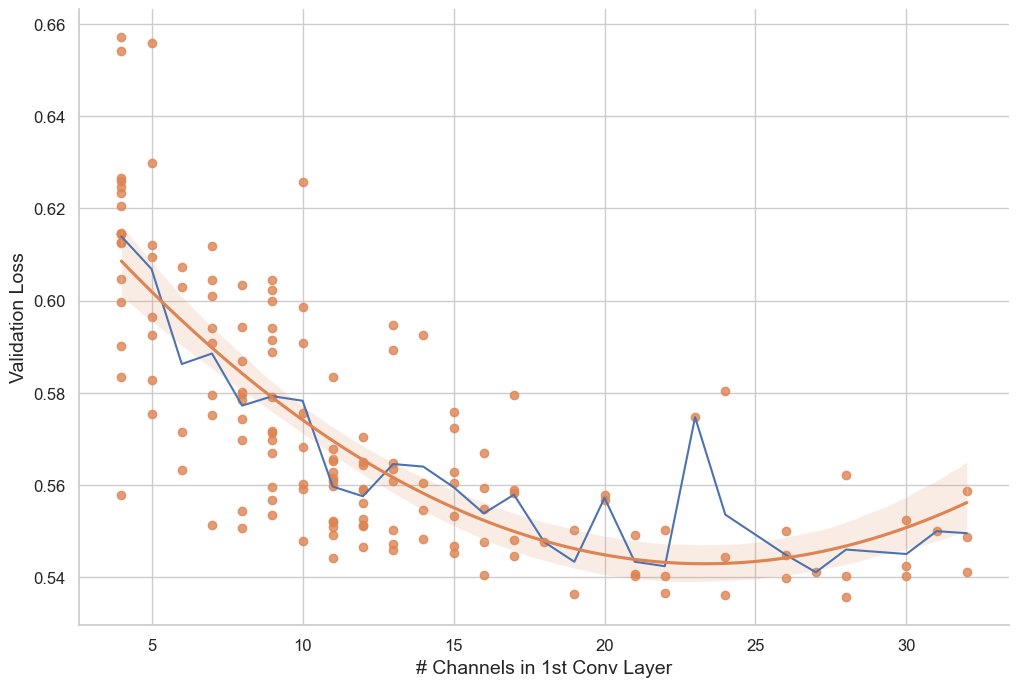
\includegraphics[width=0.48\textwidth]{figures/06_ModelExploration/4_CNN/conv_ch1.png}}}
    \subfloat[]{{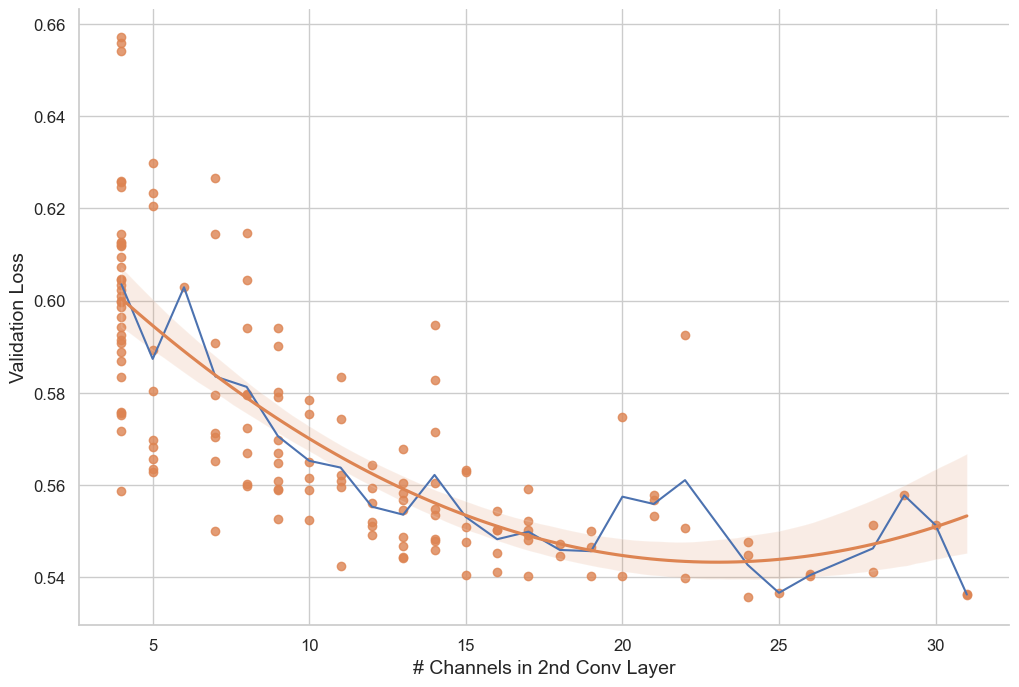
\includegraphics[width=0.48\textwidth]{figures/06_ModelExploration/4_CNN/conv_ch2.png}}}
    \caption{Influence of the number of channels in the first (a) and second (b) convolutional layers on \( \lossCEVal \).}
    \label{fig:ch1ch2}
\end{figure}

\begin{figure}[H]
    \centering
    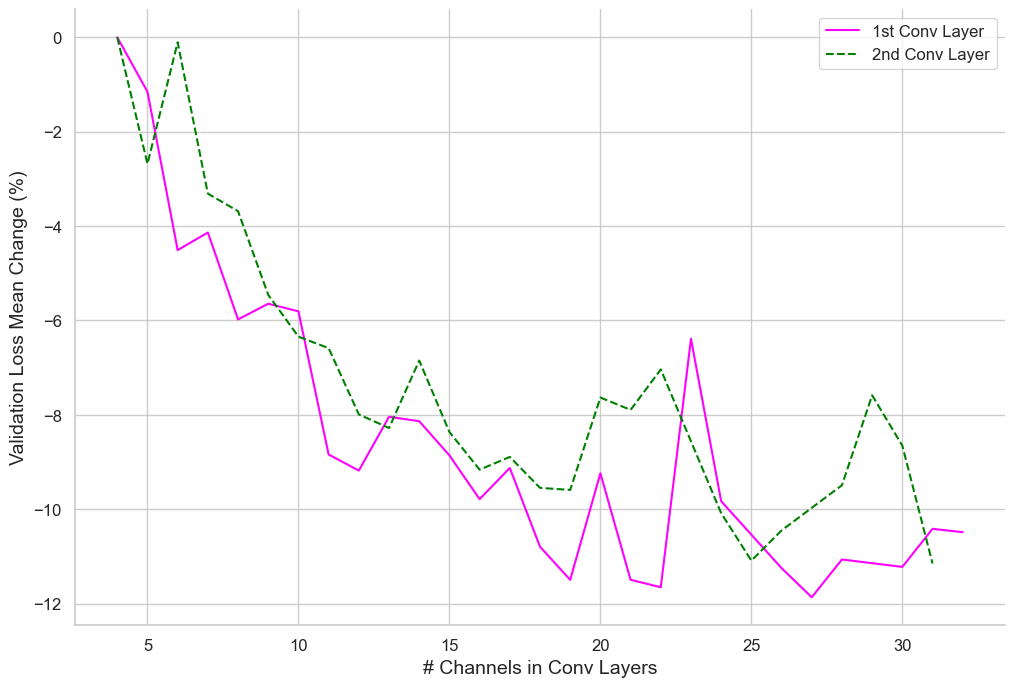
\includegraphics[width=0.5\textwidth]{figures/06_ModelExploration/4_CNN/conv_ch_change.png}
    \caption{Relative changes in validation loss for varying number of channels in both conv blocks.}
    \label{fig:ch1ch2_relchange}
\end{figure}

Figures~\ref{fig:ch1ch2} and~\ref{fig:ch1ch2_relchange} illustrate how varying the number of channels affects model
performance, guiding the selection towards an optimal balance that maximizes feature extraction while minimizing the
likelihood of overfitting.\\
Both figures indicate that the explored ranges of channels \( C_{\text{out}} \) were chosen appropriately, given that
the validation loss \( \lossCEVal \) exibits a local minimum, beyond which the loss increases due to overfitting. \\

\textbf{Pooling Layers} complement convolutional layers by reducing the spatial dimension of the feature maps,
thus allowing the model to capture higher-level features with a greater local dispersion. \\

The sizes of the pooling windows as well as other hyperparameters which are linked to the convolutional layers, all have
an impact on the model's performance, as depicted in Figure~\ref{fig:param_impact}.

\begin{figure}[H]
    \centering
    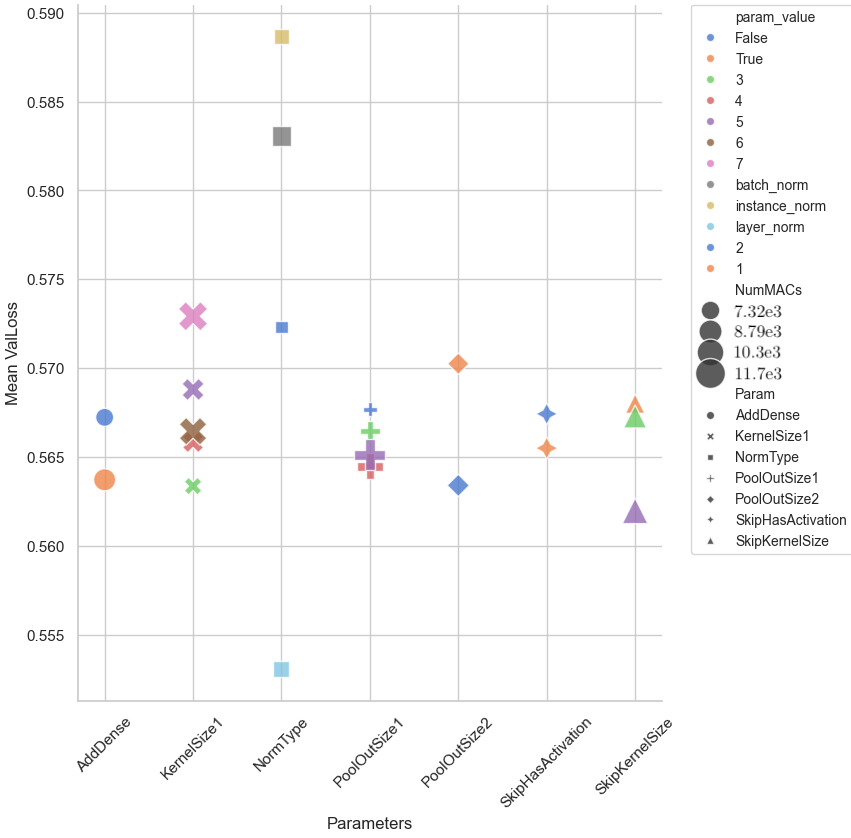
\includegraphics[width=0.6\textwidth]{figures/06_ModelExploration/4_CNN/scatter.png}
    \caption{Scatter plot showing the impact of different hyperparameters on mean validation loss.}
    \label{fig:param_impact}
\end{figure}

Figure~\ref{fig:param_impact} presents a scatter plot of various hyperparameter configurations and their corresponding
mean validation loss. Each point represents a unique combination of parameters such as kernel size, normalization type,
and pooling size. The plot indicates the sensitivities of the validation loss to these hyperparameters, with certain
configurations leading to lower loss values and thus better model performance.

The scatter plot also highlights the trade-offs between model complexity, as indicated by the size of the points
representing the number of \glspl{mac}.\\
For example, larger kernels and additional dense layers may contribute
to a lower validation loss but also increase the computational requirements. Conversely, smaller kernels and fewer dense
layers might yield a less complex model but potentially at the cost of higher validation loss.

The other depicted criteria, such as the type of normalization layer, will be discussed subsequently.

\subsubsection{Normalization Layers}
Normalization layers, crucial for modern deep networks, standardize the activations of each layer,
thus enhancing the optimization process and the network's generalization capabilities. \\
Even in shallow networks, normalization proves beneficial, as it stabilizes the gradient flow by reducing the sharpness
of the loss surface. \\
A smoother loss surface is associated with a reduced risk of overfitting since it is less likely
to contain sharp local minima, which are more prone to overfitting and generally hinder the optimization process~\cite{lyu2023norm}.\\
Another advantage is the reduction of the internal covariate shift, which is the change in the distribution of network's activations during training, as
well as the consequent potential for faster convergence through the employment of larger learning rates. \\

In the context of this work, three normalization layers were considered: Batch Normalization, Instance Normalization,
and Layer Normalization, each visualized in~\autoref{fig:all_norm_types}.

\begin{figure}[H]
    \centering
    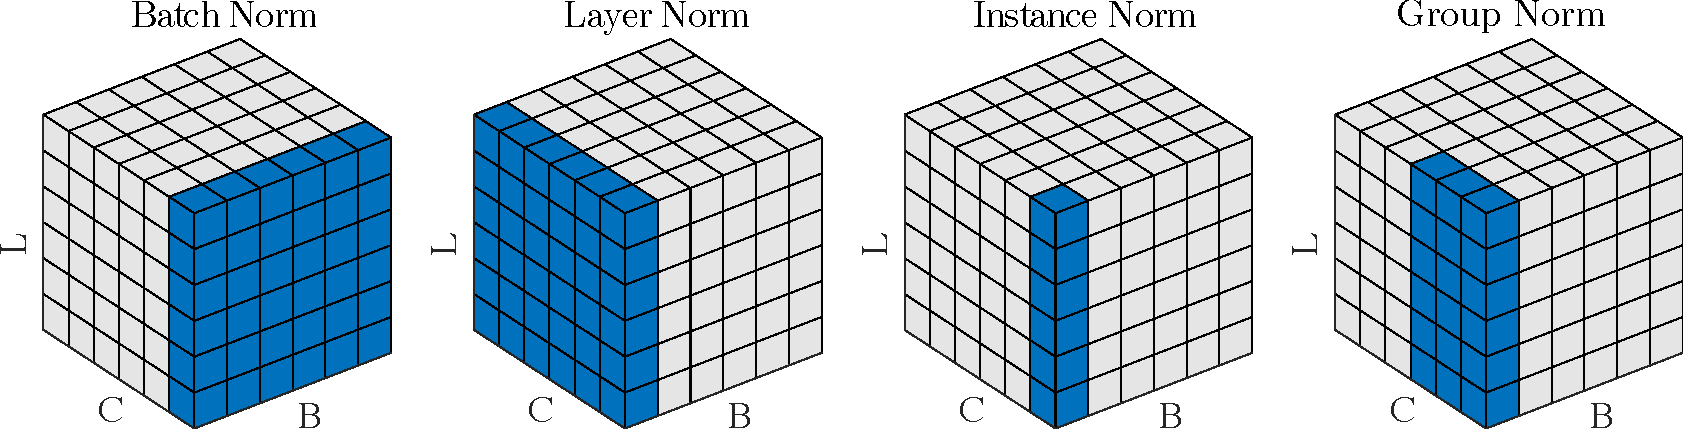
\includegraphics[width=0.6\textwidth]{figures/06_ModelExploration/4_CNN/all_norms.pdf}
    \caption{Feature map tensors -- blue units are normalized by the same mean and variance~\cite{wu2018group}.}
    \label{fig:all_norm_types}
\end{figure}

Although, Group Normalization was not considered in this work, it is worth mentioning it, since it was shown to outperform
the other normalization layers in the context of small batch sizes~\cite{wu2018group}, while being on par with Group Norm for larger batch
sizes, while exhibiting no dependence on the batch size. \\
Batch Normalization computes statistics (\(\mathbb{E}[\bfm{X}], \operatorname{Var}[\bfm{X}]\)) across the spatial
dimensions and all samples in the mini-batch for each channel, Layer Normalization along the \((L, C)\) axes for each
sample, and Instance Normalization along the \(L\) axis for each sample and channel~\cite{wu2018group}.

They all aim to compensate for the possible loss of representational capacity by introducing a learnable linear
transformation, parametrized by \( \bfm{\gamma} \) and \( \bfm{\beta} \),
that scales and shifts the normalized value~\cite{wu2018group}, expressed for Layer Normalization as~\cite{PyTorchLayerNorm}:
\begin{equation}
    \bfm{Y}_{b, :, :} = \bfm{\gamma} \odot \left( \frac{\bfm{X}_{b, :, :} - \mathrm{E}[\bfm{X}_{b, :, :}]}{\sqrt{\operatorname{Var}[\bfm{X}_{b, :, :}] + \epsilon}} \right) + \bfm{\beta}, \quad \text { where } \bfm{\gamma}, \bfm{\beta} \in \mathbb{R}^{C \times L}
\end{equation}

The validation loss for each normalization layer is depicted in~\autoref{fig:norm_type}.
\begin{figure}[H]
    \centering
    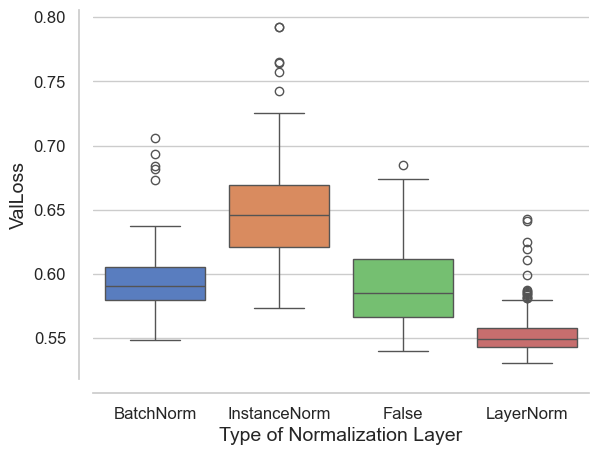
\includegraphics[width=0.6\textwidth]{figures/06_ModelExploration/4_CNN/conv_norm_type.png}
    \caption{Validation loss for different normalization layers.}
    \label{fig:norm_type}
\end{figure}

As shown in~\autoref{fig:norm_type}, the application of layer normalization (Layer Norm) resulted in the lowest \( \meanLossCEVal \),
while Instance Norm and Batch Norm performed worse. The respective layer's impacts on the model's performance and complexity
are summarized in~\autoref{tab:norm_type}.

\begin{table}[H]
    \centering
    \caption{Comparison of different normalization layers and their effects on mean validation loss and model complexity.}
    \label{tab:norm_type}
    \begin{tabular}{@{}lcccccccc@{}}
    \toprule
    & \multicolumn{2}{c}{\( \meanLossCEVal \) } & \multicolumn{2}{c}{\( \meanAccVal \)} & \multicolumn{2}{c}{\#Params} & \multicolumn{2}{c}{\#MACs} \\
    \cmidrule(lr){2-3} \cmidrule(lr){4-5} \cmidrule(lr){6-7} \cmidrule(lr){8-9}
    Normalization & \( \nu \) & \( \%\Delta \) & \( \nu \) & \( \%\Delta \) & \( \nu \) & \( \%\Delta \) & \( \nu \) & \( \%\Delta \) \\
    \midrule
    None               & 0.590 & —            & 0.737 & —            & 2322 & —    & 7.01e3 & — \\
    Batch Norm          & 0.596 & \rdbx{+0.98\%} & 0.732 & \rdbx{-0.573\%} & 2787 & \rdbx{+20.0\%} & 10.7e3 & \rdbx{+53.6\%} \\
    Instance Norm       & 0.648 & \rdbx{+9.91\%} & 0.712 & \rdbx{-3.31\%}  & 2858 & \rdbx{+23.1\%} & 10.6e3 & \rdbx{+52.3\%} \\
    Layer Norm          & 0.553 & \gnbx{-6.16\%} & 0.748 & \gnbx{+1.61\%}  & 3414 & \rdbx{+47.0\%} & 9.52e3 & \rdbx{+35.8\%} \\
    \bottomrule
    \end{tabular}
\end{table}


The underwheling performance of Instance Norm is likely due its inherent unsuitablity for the task at hand, given that
it was originally designed for style transfer and image generation tasks and generally requires larger spatial or temporal
dimensions to effectively estimate the mean and variance of the input data.
Moreover, Instance Norm was \emph{not} implemented with the subsequent affine transformation, which also contributed to its
underperformance.\\
Layer Norm has demonstrated its capability to address various shortcomings of Batch Norm~\cite{ba2016layer}, although
such shortcomings were not expected to be significant in this context.

Surprisingly, Batch Norm's performance was not as strong as anticipated, despite its common application in \gls{cnn} architectures
and the use of a relatively large batch size \( \B = 1024 \). The most likely explanation is that the optimization process
was conducted with a dropout rate of eight percent in each convolutional block.
Since both Batch Norm and Dropout layers introduce noise to the optimization process, their combined use could have
hindered optimal convergence. \\
It would be worthwhile to investigate Batch Norm's performance without the inclusion of dropout layers, as it is
hypothesized to surpass Layer Norm's performance when considering the large batch size~\cite{wu2018group}.


Layer Norm distinguished itself among the normalization techniques evaluated, offering superior model performance and lower complexity. \\
The advantage of Layer Norm over Batch Norm, in terms of the number of \glspl{mac}, seems paradoxical.
Batch Norm separates the entire mini-batch into \( C \) independent normalization groups, whereas Layer Norm normalizes
each sample independently. Considering that \( \B \gg C \), and \( \text{\#Params}_{\text{LN}} = L \cdot \text{\#Params}_{\text{BN}} \),
this result appears counterintuitive. \\



\subsubsection{Activation Function}
Activation functions play a critical role in neural networks, introducing non-linear properties to the system,
which allows the model to learn complex non-linear patterns in the data. The choice of activation function can
significantly affect the learning dynamics and performance of the network.

Traditionally, the \gls{relu} has been widely used due to its simplicity, effectiveness in addressing the vanishing
gradient problem, and its advantageous effects on the convergence of the optimization process over activation functions that
introduce non-zero second derivatives~\cite[Chapter 6.3.1]{dlbook}.\\
However, \gls{relu} can introduce ``dead units'', which are neurons that never activate, and therefore bring no contribution
to the network's discriminative and predictive capabilities.\\
To overcome this, variations like leaky \gls{relu}, \gls{prelu} and \gls{elu} have been proposed, which allow a small,
positive gradient for negative input values, thus preventing the issue of dead units and allowing higher learning rates~\cite{dyingRelu}.

The equations defining each activation function are as follows:

\begin{align}
    \texttt{ReLU}(x) &= \max(0, x) \label{eq:relu} \\
    \texttt{PReLU}(x) &= \begin{cases}
        x & \text{if } x > 0 \\
        \alpha x & \text{if } x \leq 0
    \end{cases}, \quad \text{where } \alpha \text{ is a learnable parameter} \label{eq:prelu} \\
    \texttt{ELU}(x) &= \begin{cases}
        x & \text{if } x > 0 \\
        \alpha \left( e^x - 1 \right) & \text{if } x \leq 0
    \end{cases}, \quad \text{where } \alpha = 1 \text{ per default}\label{eq:elu}
\end{align}

\begin{figure}[H]
    \centering
    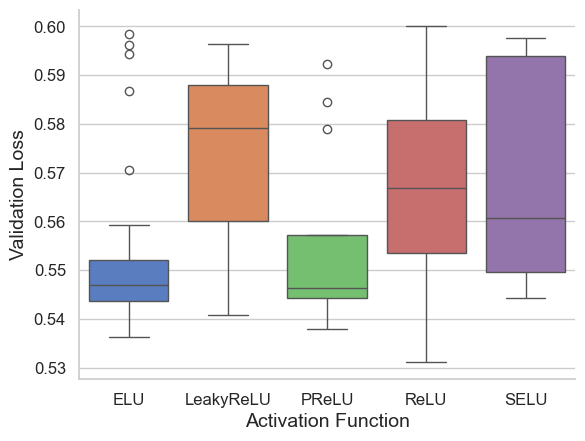
\includegraphics[width=0.55\textwidth]{figures/06_ModelExploration/4_CNN/activ_fn.png}
    \caption{Boxplots of \( \lossCEVal \) for different activation functions.}
    \label{fig:activ_fn}
\end{figure}

\autoref{fig:activ_fn} demonstrates the influence of activation functions on model performance through the distribution
of validation loss. Among the evaluated functions, \gls{prelu} and \gls{elu} show a slight advantage over \gls{relu} in terms of validation
loss, indicating potential improvements in learning dynamics and model robustness. \\
The advantages of \gls{prelu} and \gls{elu} over \gls{relu} are further quantified in \autoref{tab:activation_fn}.

\begin{table}[H]
    \centering
    \caption{Comparison of Validation Loss for Different Activation Functions}
    \label{tab:activation_fn}
    \begin{tabular}{@{}lcc@{}}
    \toprule
    Activation Function & \multicolumn{2}{c}{\( \meanLossCEVal \) } \\
    \cmidrule(lr){2-3}
                      & \( \nu \) & \( \%\Delta \) \\
    \midrule
    \gls{relu}    & 0.567 & —           \\
    \gls{prelu}   & 0.555 & \gnbx{-2.10} \\
    \gls{elu}     & 0.551 & \gnbx{-2.69} \\
    \bottomrule
    \end{tabular}
\end{table}

\gls{elu}'s smoother transition from negative to positive inputs theoretically benefits learning dynamics but
comes at a higher computational cost due to the exponential function, which might be disadvantageous for deployment on resource-constrained platforms like \glspl{fpga}.
Conversely, \gls{prelu} offers a compromise by introducing a learnable parameter, \( \alpha \), that adjusts the slope for negative inputs, offering flexibility without
significantly increasing computational demands. For this reason, \gls{prelu}, with a single shared \(\alpha\) parameter across
channels, is chosen for its balance between performance improvement and computational efficiency.
This consideration ensures that the selected activation function optimizes learning while remaining feasible for deployment
on resource-constrained platforms.

\subsubsection{The Resulting CNNP Block}
\label{subsubsec:cnn_block}

The construction of the \texttt{CNNP} block represents a synthesis of empirical findings from the exploratory process
and theoretical considerations, yielding a composite layer structure within the convolutional neural network framework.

It comprises a sequential arrangement of a one-dimensional convolutional layer (\texttt{nn.Conv1d}), followed by a
layer normalization module (\texttt{nn.LayerNorm}), a parametric rectified linear unit (\texttt{nn.PReLU}), and an
adaptive max pooling layer (\texttt{nn.AdaptiveMaxPool1d}), concluding with a dropout layer to mitigate overfitting.

\[
    \texttt{CNNP} \coloneqq \underbrace{\texttt{nn.Conv1d}}_{\text{\textbf{C}onv}}
    \rightarrow \underbrace{\texttt{nn.Layer Norm}}_{\text{\textbf{N}orm}}
    \rightarrow \underbrace{\texttt{nn.PReLU}}_{\text{\textbf{N}on-linear}}
    \rightarrow \underbrace{\texttt{nn.AdaptiveMaxPool1d}}_{\text{\textbf{P}ool}}
    \rightarrow \texttt{nn.Dropout}
\]

The dropout rate was optimized parallel to the other hyperparameters, depicted in~\autoref{fig:param_impact}, and its
impact on the model's performance can be found in the appendix~\autoref{fig:dropout_cnn}.


\subsubsection{Skip Connection}

Skip connections, are a fundamental architectural feature in deep neural networks that enable the training of significantly
deeper models by providing advantageous optimization trajectories through the loss landscape or allowing for the reuse or
preservation of important features throughout the network. \\
The most prominent example of a skip connection is the residual connection, which was first introduced in the ResNet architecture~\cite{he2015deep}.
Residual connections aim to address the degradation problem, which is the phenomenon where increasing the depth of a network
results in higher training error due to various optimization difficulties. \\
The application of residual connections mostly aims to achieve better optimization dynamics by reformulating the
bypassed layers' training objectives to learn the residual (\( \coloneq \) difference) from the identity mapping, instead
of learning an unreferenced mapping from scratch.

Since the phenomenon of degradation is more prevalent in very deep networks, which might be up to 2 orders of magnitude deeper
than our model, the use of skip connections is not motivated by the degradation problem, but rather by the goal to allow
for more diverse feature representations.
The use of skip connections in our model architecture is motivated by the
desire to create an ensemble of the two parallel paths, which can be seen as an ensemble of the serially connected
\texttt(CNNP)s and a layer that performs the operation formalized in~\autoref{eq:skip_connection}.
\begin{equation}
    \bfm{X}_{:, j}^{\text{(skip)}} = \texttt{ReLU}\left(\text{bias}_j + \sum_{k=0}^{M} \bfLT_{:, k, 1}^P \cdot W_{jk}\right), \quad  \bfm{X}^{\text{(skip)}} \in \mathbb{R}^{\B \times C_{\text{out}}^{(\text{skip})}}, \: j = 1, \ldots, C_{\text{out}}^{(\text{skip})}
    \label{eq:skip_connection}
\end{equation}
The input to the skip connection is the permuted tensor of eigenvalues \( \bfLT^P \coloneqq \texttt{permute}( \bfLT, [0, 2, 1] ) \).
\( C_{\text{in}}^{(\text{skip})} = M = \| \bfL \| \) is the number of input channels, \( C_{\text{out}}^{(\text{skip})} \)
is the number of output channels, and \( \bfm{W} \) are the weights of the \( 1 \times 1 \) convolutional layer in the
skip connection.

In contrast to a residual connection, the outputs of our skip connection \( \bfm{X}^{\text{(skip)}} \) are not
added to the outputs of the ``main'' path, but are concatenated to them. \\
Adding the outputs of the skip connection and the main path requires both operands to exhibit the same dimensions, which is
not the case in our model architecture. Moreover, concatenation preserves a more diverse feature representation since
it allows both paths to learn different features, rather than simplifying the learning task by allowing the model to
learn the residual from the identity mapping. \\

\begin{table}[H]
    \centering
    \caption{Comparison of model performance with and without skip connections}
    \label{tab:residual_comparison}
    \begin{tabular}{@{}lcccccccc@{}}
    \toprule
    & \multicolumn{2}{c}{\( \meanLossCEVal \) } & \multicolumn{2}{c}{\( \meanAccVal \)} & \multicolumn{2}{c}{\#Params} & \multicolumn{2}{c}{\#MACs} \\
    \cmidrule(lr){2-3} \cmidrule(lr){4-5} \cmidrule(lr){6-7} \cmidrule(lr){8-9}3
    Skip Connection & \( \nu \) & \( \%\Delta \) & \( \nu \) & \( \%\Delta \) & \( \nu \) & \( \%\Delta \) & \( \nu \) & \( \%\Delta \) \\
    \midrule
    None & 0.544 & - & 0.753 & - & 2667 & - & 8984 & - \\
    Skip & 0.545 & \rdbx{0.296} & 0.751 & \rdbx{-0.183} & 2721 & \rdbx{2.02} & 9038 & \rdbx{0.601} \\
    Skip \( \oplus \) Conv & 0.537 & \gnbx{-1.28} & 0.756 & \gnbx{0.435} & 2747 & \rdbx{3.00} & 9036 & \rdbx{0.568} \\
    \bottomrule
    \end{tabular}
\end{table}

\autoref{tab:residual_comparison} shows the comparison of model performance with and without the skip connection. The second
column ``Skip'' refers to a model, in which the output of the serially connected \texttt{CNNP} blocks is concatenated with
the original input tensor of eigenvalues.
The third column ``Skip \( \oplus \) Conv'' refers to the model with skip connections as introudced in~\autoref{eq:skip_connection},
and depicted in~\autoref{fig:cnn_architecture}.\\
\autoref{fig:ch_skip} shows the influence of the number of channels in the skip connection \( C_{\text{out}}^{(\text{skip})} \) on
the validation loss \( \lossCEVal \).

\begin{figure}[H]
    \centering
    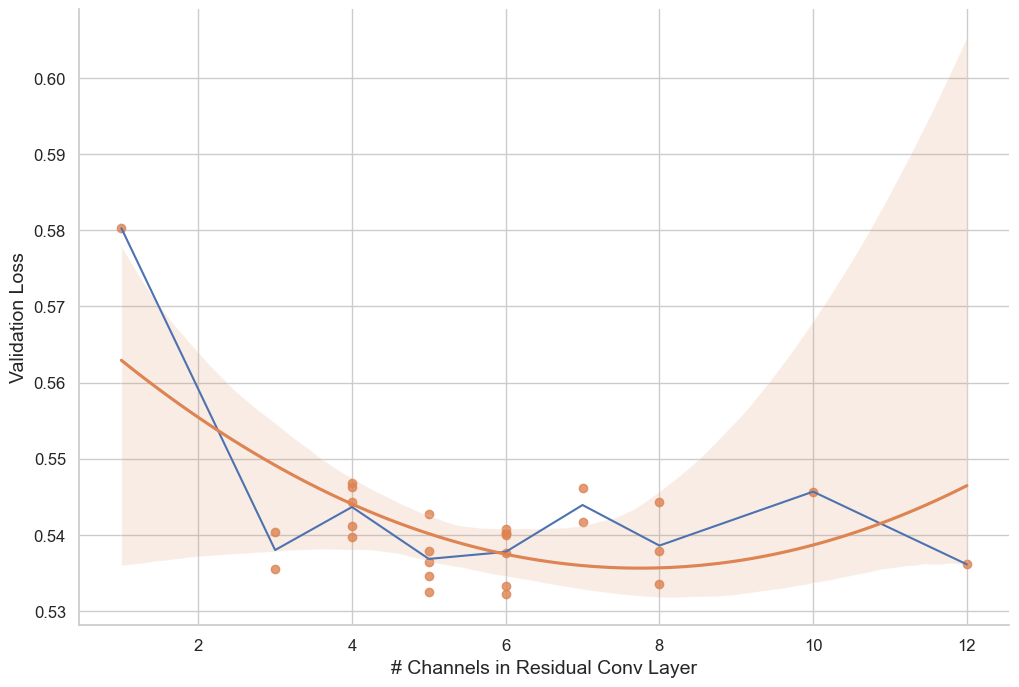
\includegraphics[width=0.45\textwidth]{figures/06_ModelExploration/4_CNN/conv_chskip.png}
    \caption{Influence of the number of channels in the skip connection.}
    \label{fig:ch_skip}
\end{figure}

Given the low number of optimization trials used to evaluate  \( C_{\text{out}}^{(\text{skip})} \), we decided to choose
a more conservative value of \( C_{\text{out}}^{(\text{skip})} = 5 \) to avoid overfitting. \\
Empirical evidence indicated a marginal performance increase when applying the \gls{relu} activation function to the
output of the skip connection. Its application post-concatenation introduces non-linearity that helps in the differentiation
and processing of features. Given its low
computational overhead and subtle positive impact on model performance, we decided to apply ReLU to our skip connections, thereby
leveraging the advantages of non-linearity while maintaining computational efficiency.

\paragraph{Varying Snapshot Count}
\hyperref[fig:cnn_plus_arch]{Figure~\ref*{fig:cnn_plus_arch}} conceptualizes the adaptation of the employed CNN architecture to handle a variable number
of snapshots by embedding the number of snapshots \( K \) into the skip branch of the network.
The results of the evaluation of the model with varying snapshot count will be presented in~\autoref{sec:influence_num_snapshots}.

\subsection{Resulting Architecture}
\label{subsubsec:resulting_architecture}

The development of the \gls{cnn} architecture, delineated in~\autoref{fig:cnn_architecture}, was achieved through a
methodical hyperparameter optimization facilitated by \textsc{Optuna}.
The optimization targeted a multidimensional objective function that accounted for validation loss (\( \meanLossCEVal \)),
model complexity (number of parameters and \glspl{mac}), and validation accuracy (\( \meanAccVal \)).

\begin{figure}[H]
    \centering
    \subfloat[]{{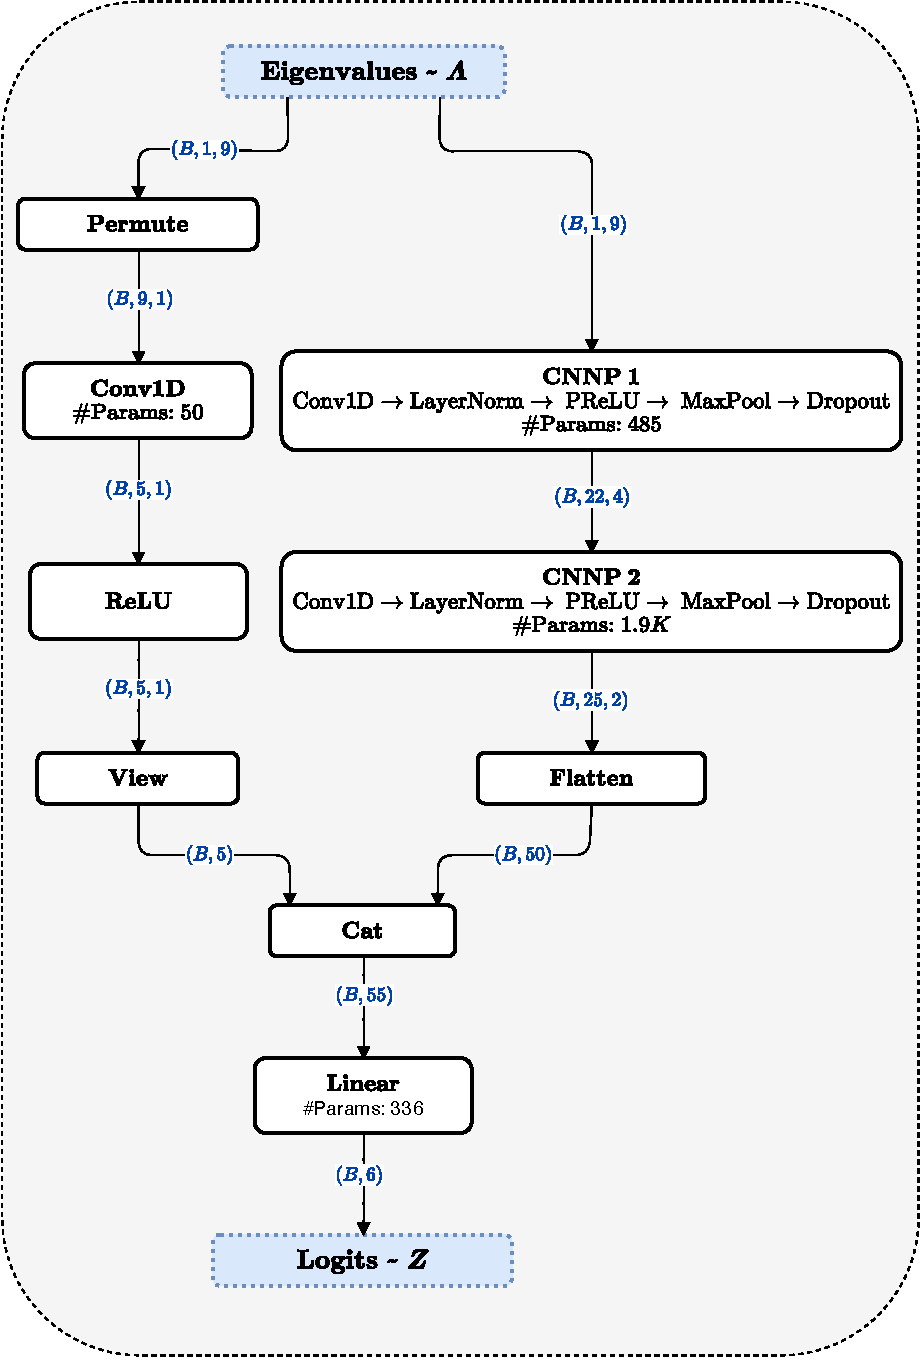
\includegraphics[width=0.41\textwidth]{figures/06_ModelExploration/4_CNN/cnn.pdf}}}
    \hspace{0.5cm}
    \subfloat[\label{fig:cnn_plus_arch}]{{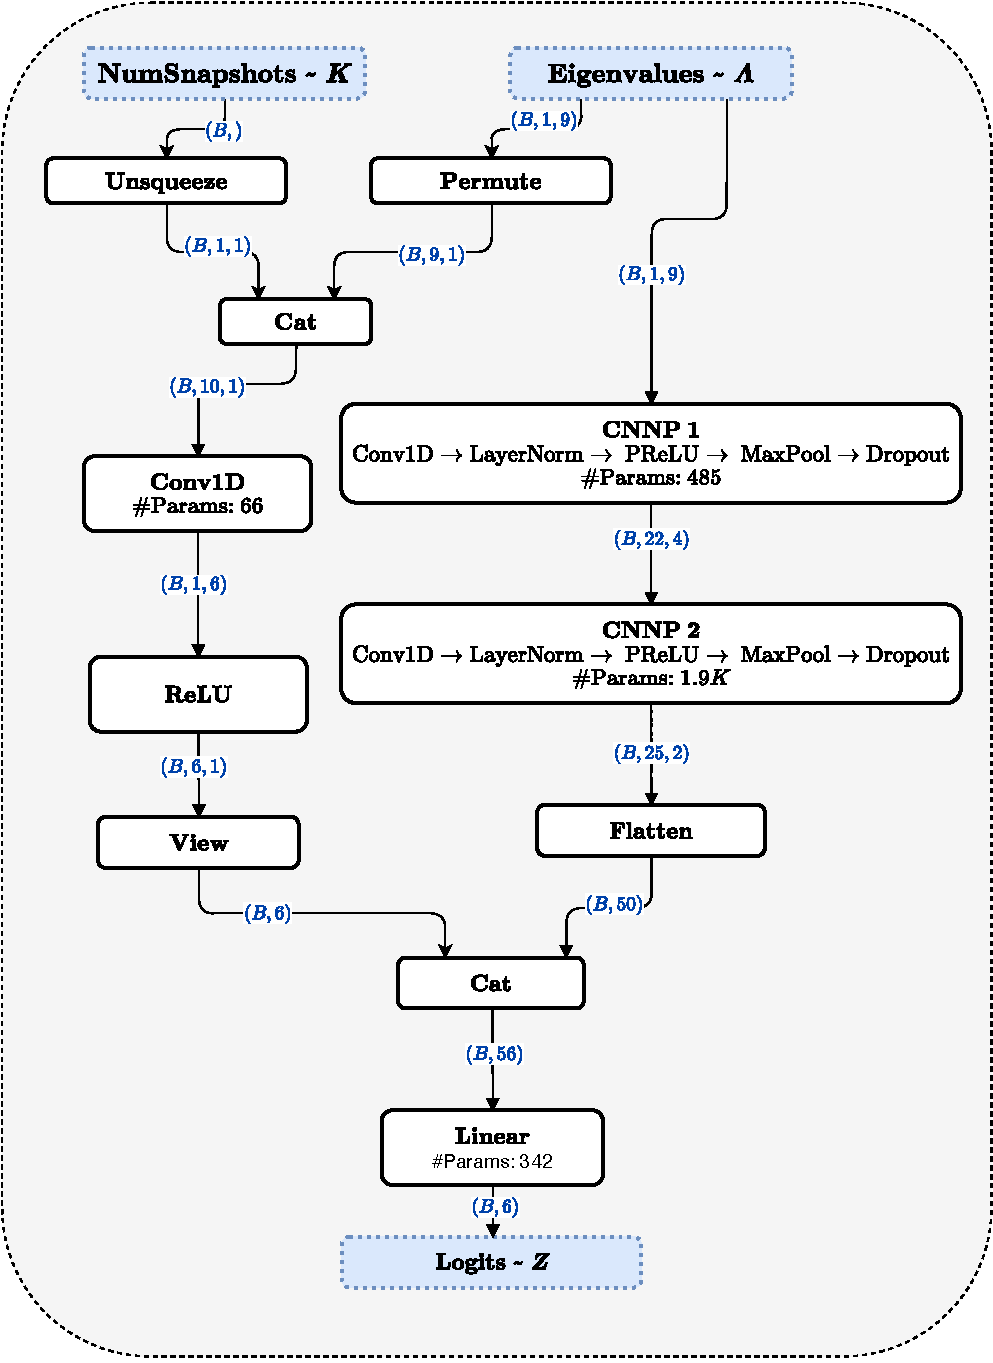
\includegraphics[width=0.44\textwidth]{figures/06_ModelExploration/4_CNN/cnn+.pdf}}}
    \caption{Schematic of the \gls{cnn} (a) and its variable snapshot adaptation (b).}
    \label{fig:cnn_architecture}
\end{figure}

The decision to employ a series connection of two \texttt{CNNP}'s in the ``main'' path can be attributed to the length
of the input sequence \( L_{\text{seq}} = M\), which is short enough, such that two \texttt{CNNP} blocks with kernel
sizes of three in combination with the adaptive max pooling%
\footnote{The dimensional reductions are denoted in~\autoref{tab:cnn_summary}}
layers can effectively capture relevant features at all spatial scales. \\
Experimental evaluations indicated that the addition of a third \texttt{CNNP} block without intermediate pooling did not
affect performance, while a singular \texttt{CNNP} block increased validation loss.

Detailed hyperparameters and layer configurations that underpin the network's structure and training methodology are
summarized in~\autoref{tab:cnn_summary}.

\begin{table}[H]
    \centering
    \caption{Summary of Hyperparameters and Layer Configurations}
    \label{tab:cnn_summary}
    \resizebox{\textwidth}{!}{%
    \begin{tabular}{@{}lll@{}}
    \textbf{Block / Module}               & \textbf{Child}        & \textbf{Parameters / Value}            \\ \midrule
    \multicolumn{3}{l}{\textbf{Modules}}                                                     \\ \midrule
    \multirow{7}{*}{\texttt{CNNP} Block 1}
                                         & \texttt{nn.Conv1d}           & Channels: \(1 \rightarrow 22\), Kernel Size: 3, Padding: \texttt{reflect} \\
                                         &                              & \#Params \( = C_{\text{in}} \times C_{\text{out}} \times k + C_{\text{out}} = 88\) \\
                                         & \texttt{nn.Layer Norm}        & \#Params \( = 2 \times C_{\text{out}} \times L_{\text{seq}} = 396 \) \\
                                         & \texttt{nn.PReLU}                & \#Params = 1            \\
                                         & \texttt{AdaptiveMaxPool1d}&  \(L_{\text{seq}} : 9 \rightarrow 4 \)                   \\
                                         & \texttt{nn.Dropout}          & Rate: 0.06                      \\
                                         & \( \Sigma \) \#Params                  &  \( 1 \times 22 \times 3 + 2 + 2 \times 22 \times 9 + 1 = 485 \)\\\midrule
    \multirow{7}{*}{\texttt{CNNP} Block 2}
                                         & \texttt{nn.Conv1d}           & Channels: \(22 \rightarrow 25\), Kernel Size: 3, Padding: \texttt{reflect} \\
                                         &                              & \#Params \( = C_{\text{in}} \times C_{\text{out}} \times k + C_{\text{out}} = 1675\) \\
                                         & \texttt{nn.Layer Norm}        & \#Params \( = 2 \times C_{\text{out}} \times L_{\text{seq}} = 200 \)                       \\
                                         & \texttt{nn.PReLU}                & \#Params = 1            \\
                                         & \texttt{nn.AdaptiveMaxPool1d}& \(L_{\text{seq}} : 4 \rightarrow 2 \)                   \\
                                         & \texttt{nn.Dropout}                   & Rate: 0.06                      \\
                                         & \( \Sigma \) \#Params                & \( 22 \times 25 \times 3 + 25 + 2 \times 25 \times 4 + 1 = 1876 \) \\\midrule
    \multirow{3}{*}{Skip Connection}     & \texttt{nn.Conv1d}          & Channels: \(9 \rightarrow 5\), Kernel Size: 1 \\
                                         &                              & \#Params \( = C_{\text{in}} \times C_{\text{out}} + C_{\text{out}} = 50 \) \\
                                         & \texttt{nn.ReLU}                &             \\ \midrule
    Head                                 & \texttt{nn.Linear}          & \#Params = \( (2 \times 25 + 5) \times \| \NSet \| + \| \NSet \| = 336 \) \\
    \midrule[0.1pt]
    \addlinespace[0.5cm]
    \( \Sigma \) \#Params                & \texttt{ConvNet8} & 2747 \\
    \bottomrule

    \addlinespace[1cm]
    \multicolumn{3}{l}{\textbf{Non-Layer Hyperparameters}}                                       \\ \midrule
    Optimizer                            &                           & \texttt{optim.AdamW} \\
    Batch Size                           &                           & 512                       \\
    Learning Rate                        &                           & 0.002                     \\
    Weight Decay                         &                           & 0.01685                   \\
    LR Scheduler                         &                           & \texttt{lr\_scheduler.ReduceLROnPlateau}\\
    Precision                            &                           & \texttt{32-true}     \\
    \bottomrule
    \end{tabular}%
    }
\end{table}

\autoref{tab:cnn_summary} presents the chosen hyperparameters, notably including the \texttt{AdamW} optimizer. \\
This optimizer modifies the \texttt{Adam} algorithm by applying weight decay directly to the model weights instead of
incorporating it into the gradient updates. This approach allows \texttt{AdamW} to achieve more effective regularization,
enhancing the model's generalization capabilities by decoupling weight decay from the learning rate's adaptive adjustments~\cite{loshchilov2019decoupled}.

While a batch size of 1024 was used during the optimization process, the final model was trained with a batch size of 512%
\footnote{A short optimization run yielded a batch size of \( \B = 504 \) as optimal value.},
as the latter yielded a lower validation loss. This can be attributed to the fact that lower batch sizes intorduce more noise
to the optimization process, which can be beneficial to escape sharp local minima, and thus improve the generalization capabilities.

Furthermore, we employed \texttt{ReduceLROnPlateau} as a learning rate scheduler.
A comparison with other suitable
learning rate schedulers, such as \texttt{CyclicLR}, \texttt{OneCycleLR}, and
\texttt{CosineAnnealingLR}, did not yield actionable insights, as the number of steps per epoch
was too high to effectively utilize any of these schedulers. \\
An effective way to overcome this issue will be introduced in~\autoref{subsub:training_data}.

The learning rate, weight decay and dropout rate have also been optimized. The results of this optimization process can
be found in the appendix -- see Figures~\ref{fig:dropout_cnn},~\ref{fig:lr_cnn}, and~\ref{fig:wd_cnn}. \\
The weight decay parameter was optimized solely for the \gls{cnn} and was uniformly applied to all yet to be introduced
models.

\newpage{}

\section{Multilayer Perceptron}
\label{sec:mlp}

Advancements in the field of deep learning over the past decade have underscored the superiority of convolutional
and recurrent neural networks over traditional feedforward architectures, such as the \glsfirst{mlp}.\\
This superiority largely stems from CNNs' and RNNs' inherent abilities to capture spatial and temporal dependencies within
data.
Additionally, both CNNs and RNNs employ parameter sharing mechanisms -- across space for CNNs, and across time for \glspl{rnn}
-- decreasing their susceptibility to overfitting.\\

Nonetheless, the \gls{mlp} remains a foundational architecture worth exploring. This is especially true for tasks of low
complexity, where the risk of overfitting is low and the data not inherently spatially or temporally dependent.\\
However, the \gls{mlp} architecture has not been explored as extensively as the \gls{cnn} and \gls{rnn} architectures, and
is mostly an analogue to the previously introduced \gls{cnn} architecture.\\
Hence, the deep feed forward architecture will be a composite of \texttt{MLPBlock}s, each consisting of a linear layer,
followed by a normalization layer, a non-linear activation function, and finally a dropout layer. \\

\subsection{Hyperparameter Optimization}


\subsubsection{Number of Features}
\begin{figure}[H]
    \centering
    \subfloat[\texttt{MLPBlock 1}]{{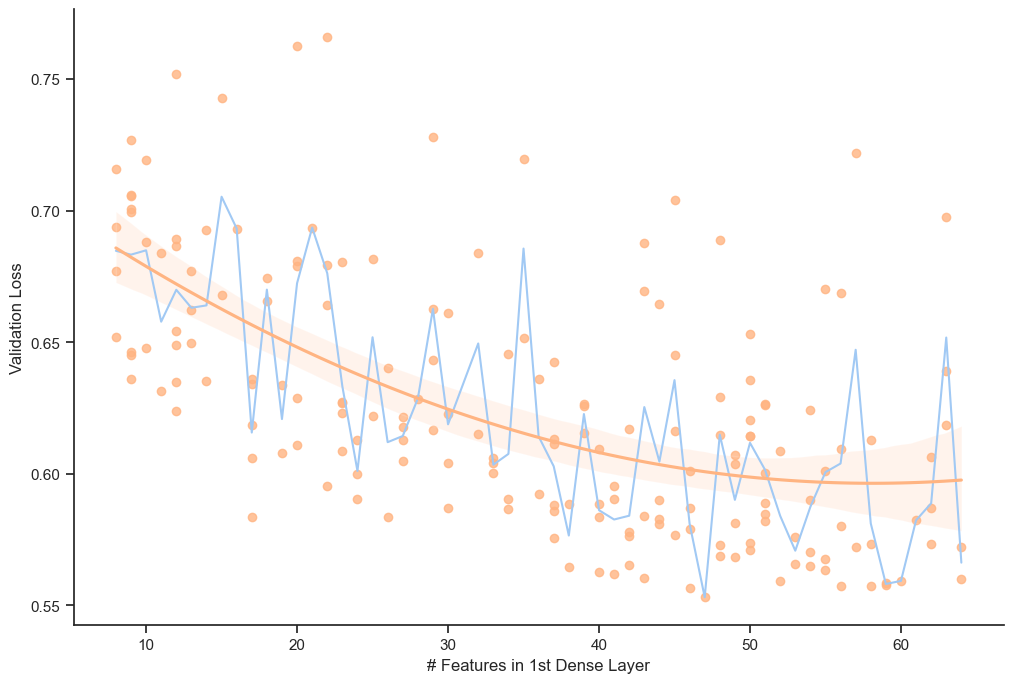
\includegraphics[width=0.33\textwidth]{figures/06_ModelExploration/5_MLP/ch1.png
    }}}
    \subfloat[\texttt{MLPBlock 2}]{{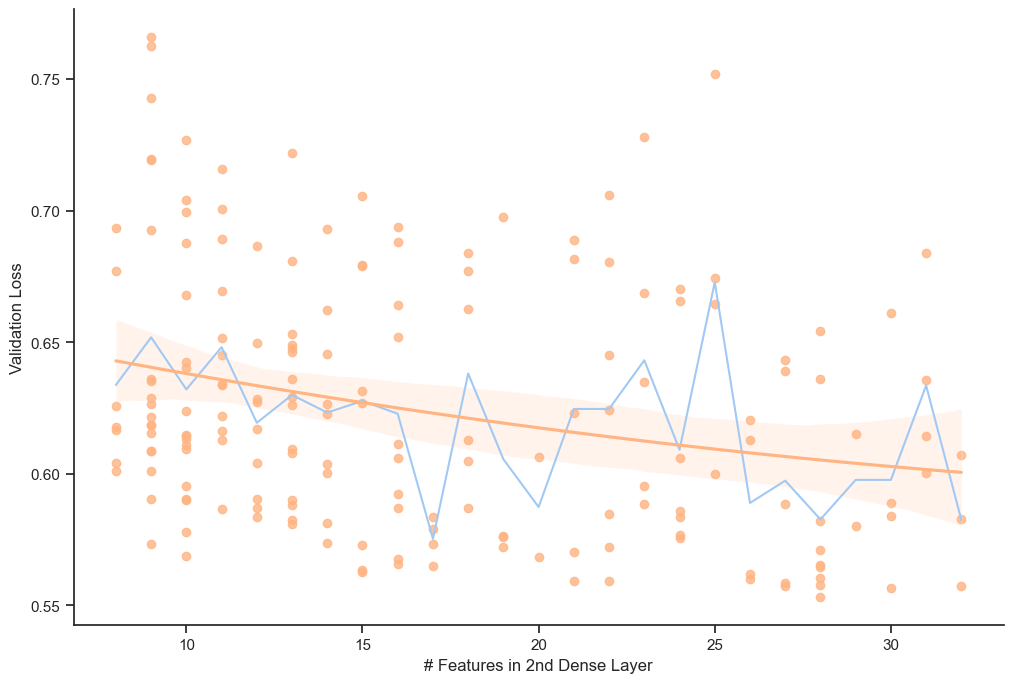
\includegraphics[width=0.33\textwidth]{figures/06_ModelExploration/5_MLP/ch2.png
    }}}
    \subfloat[\texttt{MLPBlock 3}]{{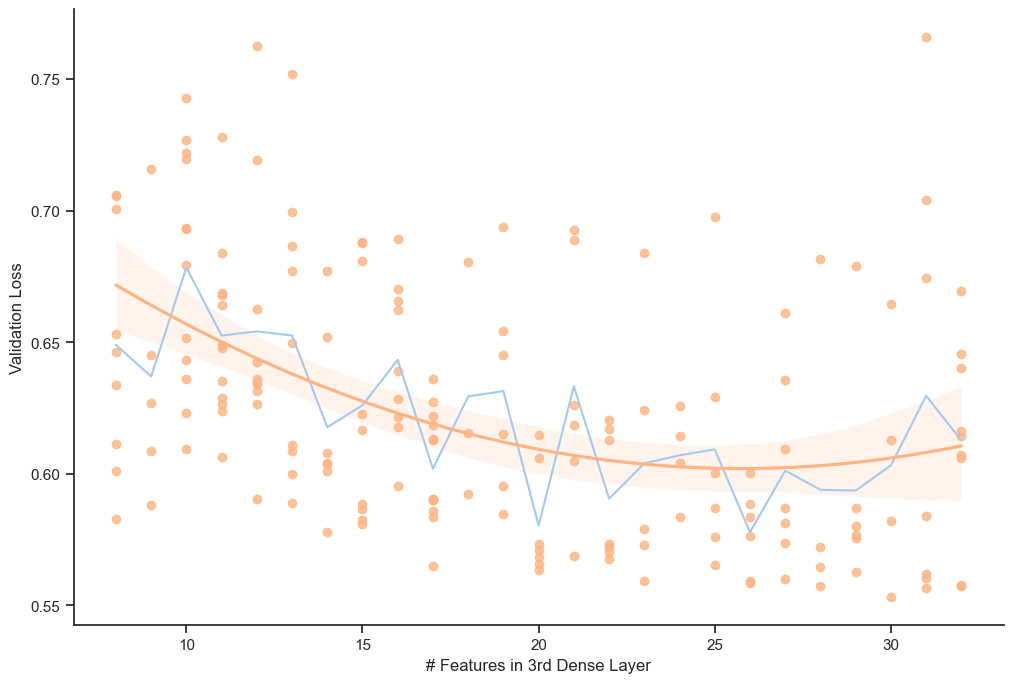
\includegraphics[width=0.33\textwidth]{figures/06_ModelExploration/5_MLP/ch3.png
    }}}
    \caption{Regression plots of the \( \lossCEVal \) for different numbers of features in the three \texttt{MLPBlock}s.}
    \label{fig:mlp_features}
\end{figure}

The exploration of the optimal number of features in the \texttt{MLPBlock}s, as depicted in \autoref{fig:mlp_features},
revealed a monotonically decreasing trend in validation loss with an increase in feature numbers for the second block, while
the first and third blocks each exhibited a local optimum within the explored range. \\
This observation suggests a higher feature count could potentially enhance model performance.
However, considering the stronger relative influence of the number of features in the first and third layers, the
feature count for the second \texttt{MLPBlock} was set to a rather conservative value of 20, to mitigate model complexity and
potential overfitting.

In retrospect, this decision seems doubious, as the subsequent \texttt{MLPBlock} contains four more features than block
two. This might cause an unwanted bottleneck effect and make some information in the last block redundant.\\


\subsubsection{Normalization and Residual Connection}

\begin{table}[H]
    \centering
    \caption{Comparison of MLP Variants}
    \label{tab:mlp_variants}
    \begin{tabular}{@{}lccccc@{}}
    \toprule
    Configuration & \multicolumn{2}{c}{\( \meanLossCEVal \)} & \multicolumn{2}{c}{\( \meanAccVal \)} \\
    \cmidrule(lr){2-3} \cmidrule(lr){4-5}
                  & \( \nu \) & \( \%\Delta \) & \( \nu \) & \( \%\Delta \) \\
    \midrule
    \multicolumn{5}{l}{Normalization} \\
    False          & 0.657 & - & 0.696 & - \\
    Batch Norm     & 0.656 & \gnbx{-0.208} & 0.706 & \gnbx{1.429} \\
    Instance Norm  & 0.621 & \gnbx{-5.567} & 0.717 & \gnbx{3.011} \\
    Layer Norm     & 0.596 & \gnbx{-9.245} & 0.728 & \gnbx{4.594} \\
    \midrule
    \multicolumn{5}{l}{Skip Connection} \\
    False          & 0.657 & - & 0.695 & - \\
    Skip           & 0.611 & \gnbx{-7.078} & 0.723 & \gnbx{4.067} \\
    \bottomrule
    \end{tabular}
\end{table}


The examination of normalization methods and skip connections within the MLP architecture reveals that both modifications
significantly influence model performance.\\
Normalization, particularly Layer Norm, markedly enhances model accuracy and reduces validation loss,
highlighting its role in stabilizing the training process and improving generalization.
Since the \gls{mlp}'s internal tensors do not exhibit separate spacial or temporal dimensions together with a channel
dimension, Instance Norm and Batch Norm aggregate their statistics in the same manner. Their difference lies in the
subsequent scaling and shifting operations.\\
While Layer Norm uses individual scaling and shifting parameters (\( \bfm{\gamma}, \bfm{\beta} \)) for each feature,
it was not possible to instantiate Instance Norm with the inclusion of the subsequent affine transformation.

The integration of skip connections also shows a notable positive effect on the model's performance.
The linear transformation within the skip branch, designed to align the feature count with the final \texttt{MLPBlock}, is then
added to the last \texttt{MLPBlock}'s output.
This addition introduces only a marginal increase in model complexity, with \( 9 \times ( 24 + 1) = 225 \) additional parameters.\\


\subsection{Resulting Architecture}
\label{sub:mlp_architecture}

The \gls{mlp} model used for testing and final comparative analysis is visualized in \autoref{fig:mlp_model}.\\
Unfortunately, the skip connection, which is highlighted in purple in the diagram, was not implemented into the final model as initially intended.

\begin{figure}[H]
    \centering
    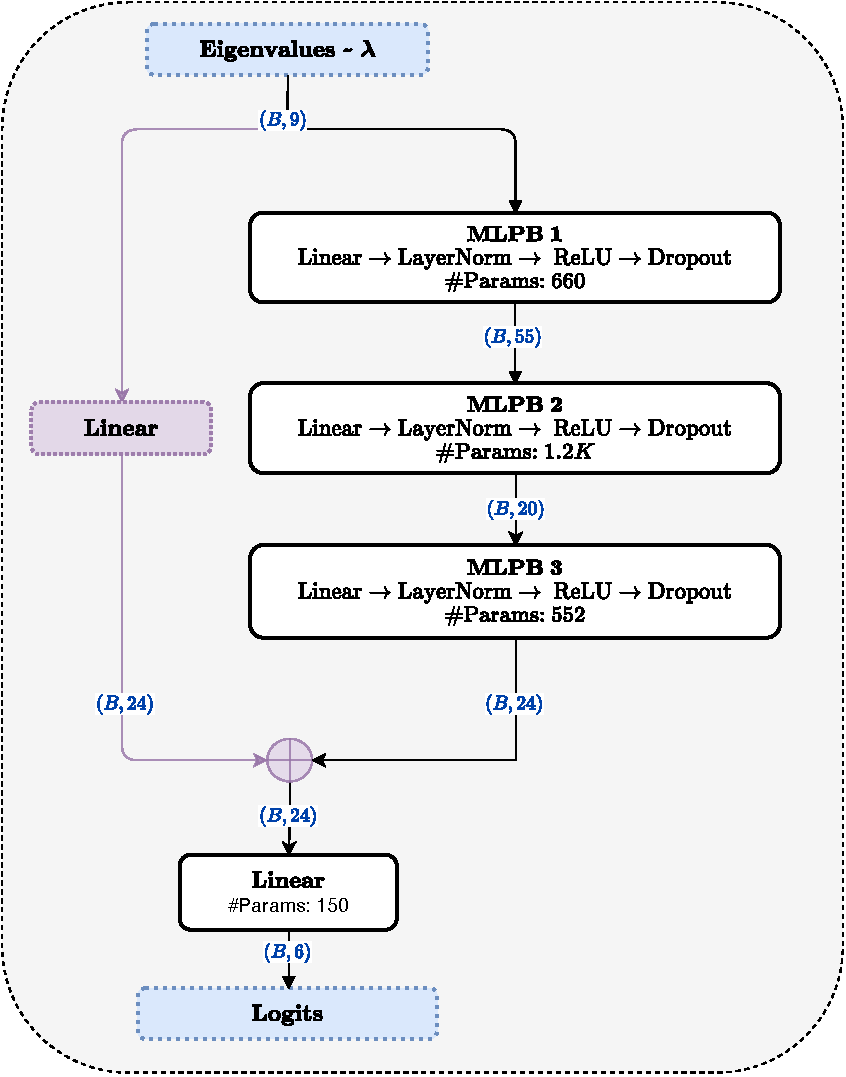
\includegraphics[width=0.45\textwidth]{figures/06_ModelExploration/mlp.pdf}
    \caption{Flowchart of the MLP architecture.}
    \label{fig:mlp_model}
\end{figure}

The architecture, as depicted, encapsulates a sequential arrangement of three \texttt{MLPBlock}s, each comprising essential
components for a feedforward network: linear transformation, normalization, activation, and regularization through
dropout.\\

\autoref{tab:mlp_summary} summarizes the hyperparameters and layer configurations of the final \gls{mlp} model.

\begin{table}
    \centering
    \caption{Summary of Hyperparameters and Layer Configurations for DenseNet}
    \label{tab:mlp_summary}
    \small
    \begin{tabular}{@{}lll@{}}
    \toprule
    \textbf{Block / Module}               & \textbf{Child}        & \textbf{Parameters / Value}            \\ \midrule
    \multicolumn{3}{l}{\textbf{Modules}}                                                     \\ \midrule
    \multirow{7}{*}{\texttt{MLPBlock} 1} & \texttt{nn.Linear}           & Features: \(9 \rightarrow 55\) \\
                                         &                              & \#Params \( = 9 \times 55 + 55 = 550\) \\
                                         & \texttt{nn.LayerNorm}        & \#Params \( = 2 \times 55 = 110\) \\
                                         & \texttt{nn.ReLU}             & \\
                                         & \texttt{nn.Dropout}          & Rate: 0.06                      \\
                                         & \( \Sigma \) \#Params        & 660 \\ \midrule
    \multirow{6}{*}{\texttt{MLPBlock} 2} & \texttt{nn.Linear}           & Features: \(55 \rightarrow 20\) \\
                                         &                              & \#Params \( = 55 \times 20 + 20 = 1120\) \\
                                         & \texttt{nn.LayerNorm}        & \#Params \( = 2 \times 20 = 40\) \\
                                         & \texttt{nn.ReLU}             & \\
                                         & \texttt{nn.Dropout}          & Rate: 0.06                      \\
                                         & \( \Sigma \) \#Params        & 1160 \\ \midrule
    \multirow{6}{*}{\texttt{MLPBlock} 3} & \texttt{nn.Linear}           & Features: \(20 \rightarrow 24\) \\
                                         &                              & \#Params \( = 20 \times 24 + 24 = 504\) \\
                                         & \texttt{nn.LayerNorm}        & \#Params \( = 2 \times 24 = 48\) \\
                                         & \texttt{nn.ReLU}             & \\
                                         & \texttt{nn.Dropout}          & Rate: 0.06                      \\
                                         & \( \Sigma \) \#Params               & 552 \\ \midrule
    Head                                 & \texttt{nn.Linear}           & \#Params \( = 24 \times \| \NSet \| + \| \NSet \| = 150\) \\
                                         &                              & \#Params = 150 \\
    \midrule[0.1pt]
    \addlinespace[0.5cm]
    \( \Sigma \) \#Params                & \texttt{DenseNet} & 2522 \\
    \bottomrule

    \addlinespace[1cm]
    \multicolumn{3}{l}{\textbf{Non-Layer Hyperparameters}}                                       \\ \midrule
    Optimizer                            &                           & \texttt{optim.AdamW} \\
    Batch Size                           &                           & 512                       \\
    Learning Rate                        &                           & 0.005                     \\
    Weight Decay                         &                           & 0.01685                   \\
    LR Scheduler                         &                           & \texttt{lr\_scheduler.ReduceLROnPlateau}\\
    Precision                            &                           & \texttt{32bit-true}     \\
    \bottomrule
    \end{tabular}
\end{table}

Without any further hyperparameter optimization, the learning rate of the final model was set to a value of
\( \alpha = 0.005 \)%
\footnote{Retrospectively, this value seems to be too high, as argumented in~\autoref{subsub:considerations_nn}.}.
The weight decay, as well as the dropout rate have been adapted from the convolutional model.\\

\subsubsection{Future Improvements}

Given the freedom of choice with respect to the number of features in the \texttt{MLPBlock}s, an adaptation worth considering
would be to align the feature count in the second \texttt{MLPBlock} to match the third could mitigate potential information
bottlenecking and enable the model to leverage a broader feature representation. This adjustment might not only harmonize
the flow of information across the layers but could also pave the way for implementing a true residual connection,
paralleling the final \texttt{MLPBlock}, to further enhance the model's learning capacity without substantially increasing its complexity.

Should the model be considered for further development, it would also be interesting to explore the impact of pruning
techniques on the model's performance.\\

The observed slight performance improvements through the use of \gls{prelu} over \gls{relu} in the convolutional model
suggest that these findings could be transferred to the \gls{mlp} model.\\

Moreover, considering the future development of the model, the application of pruning techniques could be investigated
to refine the network's architecture by identifying and eliminating redundant units or connections, thereby streamlining
the model for improved efficiency.

\section{Recurrent Neural Network}

\subsection{Hyperparameter Optimization}

This section explores the architecture of \glspl{rnn} tailored for our task. RNNs excel in processing sequential data,
making them an intuitive architectural choice under the assumption that the ordered eigenvalues should contain ``temporal'' information.\\
The section aims to investigate various architectural choices, including cell type, sequence order, and bidirectionality, to identify the
most effective configuration for the task at hand. \\
The iterative application of the same weights across sequence elements aligns well with the potential goal of using the
model in an \gls{fpga} implementation, where weight sharing can lead to significant efficiency gains.\\

Since a detailed theoretical introduction to \glspl{rnn} would be helpful for the following consideration of the effects of
certain RNN specific architecture decisions, but would
exceed the scope of this work, we refer to the literature~\cite[Chapter 10.2 ff.]{dlbook} for a comprehensive introduction to
\glspl{rnn} or to~\cite{dlcheatsheet} for a more compact overview.\\

\subsubsection{Selection of the RNN Cell Type}

Among the various \gls{rnn} cell types, the classic \gls{rnn} cell was chosen over \gls{lstm} and \gls{gru} cells. This
decsision will be substantiated through the combination of empirical findings and theoretical considerations, which will
be presented in this section.\\

\begin{figure}[H]
    \centering
    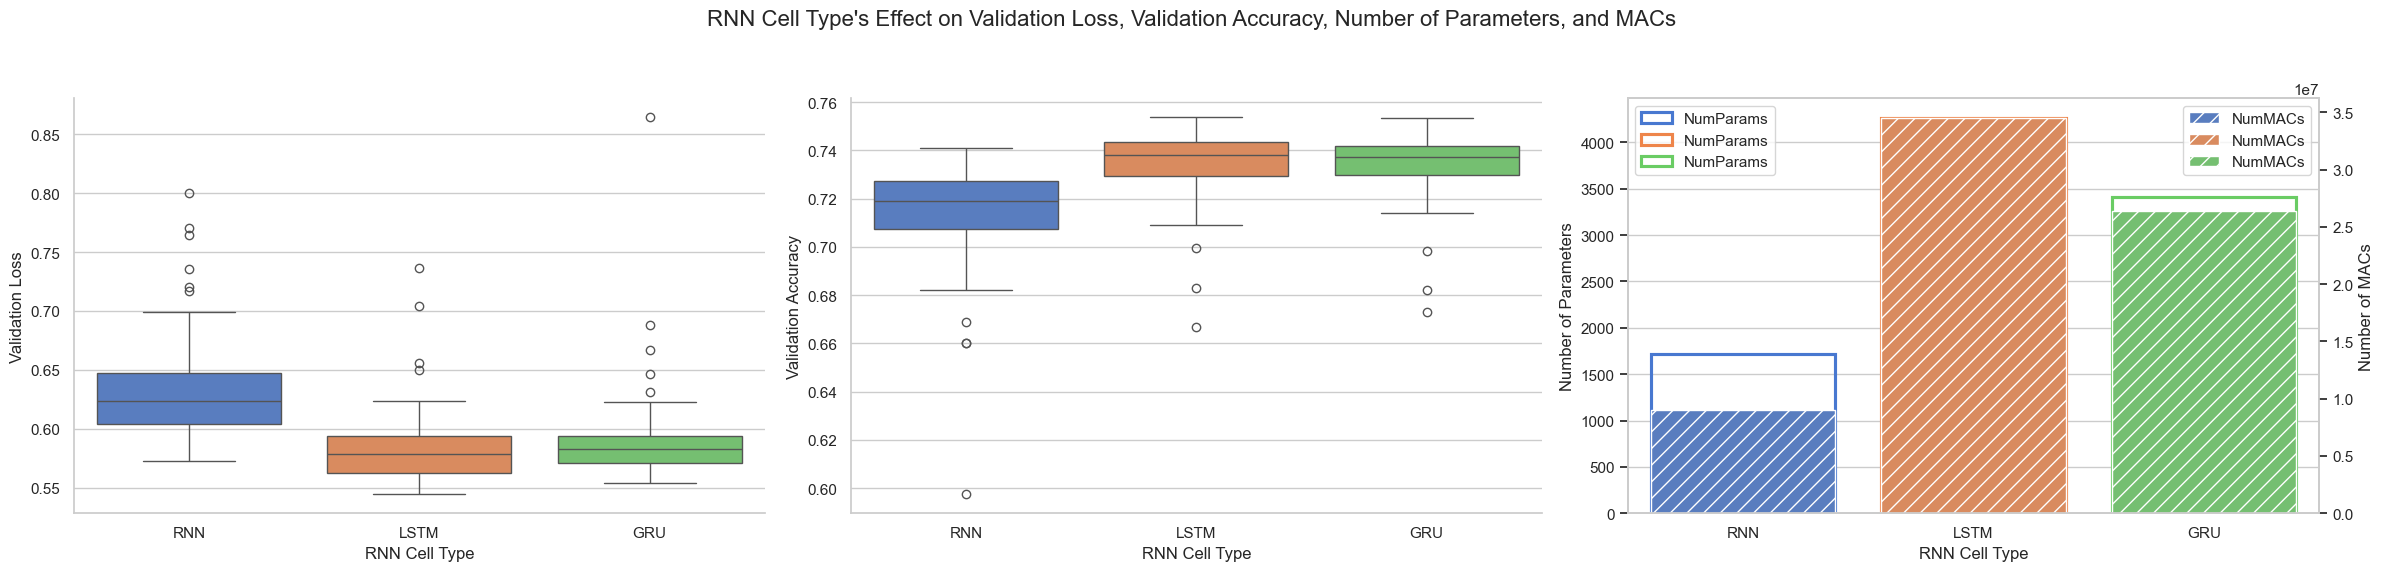
\includegraphics[width=1\textwidth]{figures/06_ModelExploration/RNN/rnn_cell_types.png}
    \caption{Comparison of RNN cell types with respect to validation loss, validation accuracy, and computational complexity.}
    \label{fig:rnn_cell_types}
\end{figure}

\begin{table}[H]
    \centering
    \caption{Comparison of Different RNN Cell Types}
    \label{tab:rnn_cell_types}
    \begin{tabular}{@{}lcccccccc@{}}
    \toprule
    & \multicolumn{2}{c}{\( \meanLossCEVal \) } & \multicolumn{2}{c}{ \( \meanAccVal \) } & \multicolumn{2}{c}{\#Params} & \multicolumn{2}{c}{\#MACs} \\
    \cmidrule(lr){2-3} \cmidrule(lr){4-5} \cmidrule(lr){6-7} \cmidrule(lr){8-9}
    RNN Cell Type & \( \nu \) & \( \%\Delta \) & \( \nu \) & \( \%\Delta \) & \( \nu \) & \( \%\Delta \) & \( \nu \) & \( \%\Delta \) \\
    \midrule
    RNN  & 0.634 & —             & 0.714 & —            & 1718 & —          & 8784  & —           \\
    GRU  & 0.591 & \gnbx{-6.72}  & 0.734 & \gnbx{2.76} & 3414 & \rdbx{98.7} & 25780 & \rdbx{193}\\
    LSTM & 0.585 & \gnbx{-7.78}  & 0.734 & \gnbx{2.84} & 4262 & \rdbx{148}  & 33700 & \rdbx{283}\\
    \bottomrule
    \end{tabular}
\end{table}

This choice is substantiated by the empirical findings presented in~\autoref{tab:rnn_cell_types} and~\autoref{fig:rnn_cell_types},
which compare the cell types based on performance and computational demands, revealing the traditional RNN cell as the most balanced option.\\
The significantly lower computational complexity of the RNN cell, compared to GRU and LSTM cells, stems from its simpler
structure without gating mechanisms. Each gate in GRU and LSTM cells—two for GRU and three for LSTM—requires its own
set of parameters and non-linear operations, specifically \( \operatorname{sigmoid} \) and \( \operatorname{tanh} \) functions.
In contrast, the traditional RNN relies on a single \( \operatorname{tanh} \) activation function, markedly reducing the
number of parameters and computational operations required.

The purpose of the gating mechanisms in GRU and LSTM cells is to manage the temporal flow of information, allowing the model to
retain or discard information as needed. This capability is particularly beneficial for long sequences with high complexity, where the
incorporation of dependencies over extended temporal horizons with varying correlations is an intricate task. Furthermore, the
vanishing gradient problem is more likely to compromise the model's ability to capture long-term dependencies.\\
However, the relatively short sequence length, determined by the number of antennas \( M \), and low complexity of our input data,
alleviate concerns related to the vanishing gradient problem or dependencies with temporal dispersion, making the traditional
RNN cell a suitable choice for the given tasks.\\

\subsubsection{Further Architectural Considerations}

The exploration of the hyperparameter space for the RNN architecture extends beyond the selection of the cell type.\\
Further architectural considerations include the sequence order, bidirectionality, and the integration of convolutional
layers for enhanced feature extraction.\\
Additionally, a fine-tuning of hyperparameters, such as the number of hidden units and learning rate was conducted. \\


\begin{figure}[H]
    \centering
    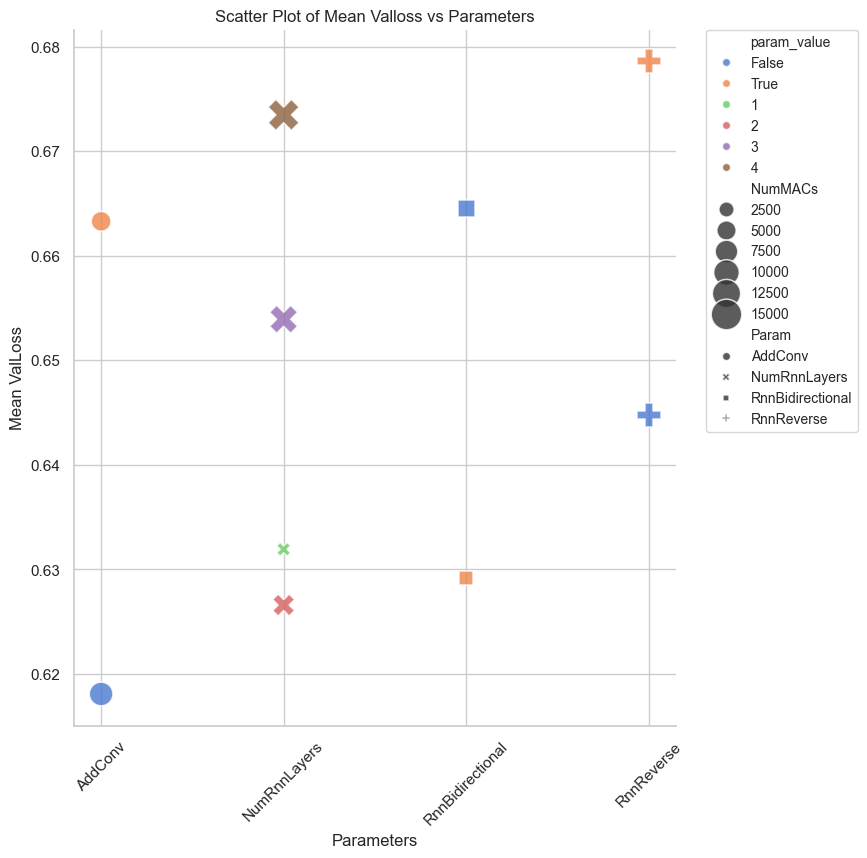
\includegraphics[width=0.6\textwidth]{figures/06_ModelExploration/RNN/rnn_scatter.png}
    \caption{Comparison of various hyperparameters with respect to the mean validation loss.}
    \label{fig:rnn_scatter}
\end{figure}

\autoref{fig:rnn_scatter} illustrates the impact of different hyperparameters on the mean validation loss \( \meanLossCEVal \) and
also aims to deliver a rather qualitative dependence of the model complexity in terms of \glspl{mac} by the marker sizes.\\
The impacts of theses architectural considerations depicted in~\autoref{fig:rnn_scatter} are furthermore gathered in~\autoref{tab:model_variants}:

\begin{table}[H]
    \centering
    \caption{Comparison of Model Variants}
    \label{tab:model_variants}
    \begin{tabular}{@{}lcccccccc@{}}
    \toprule
    & \multicolumn{2}{c}{\( \meanLossCEVal \) } & \multicolumn{2}{c}{ \( \meanAccVal \) } & \multicolumn{2}{c}{\#Params} & \multicolumn{2}{c}{\#MACs} \\
    \cmidrule(lr){2-3} \cmidrule(lr){4-5} \cmidrule(lr){6-7} \cmidrule(lr){8-9}
    Configuration & \( \nu \) & \( \%\Delta \) & \( \nu \) & \( \%\Delta \) & \( \nu \) & \( \%\Delta \) & \( \nu \) & \( \%\Delta \) \\
    \midrule[0.2pt]
    One Layer  & 0.632 &   —            &  0.717&   —            & 638  &   —           &  1830 &   —  \\
    Two Layers & 0.627 &   \gnbx{-0.844}&  0.718&   \gnbx{0.192}&  1470 &   \rdbx{130}&  6948 &   \rdbx{280}   \\
    \midrule[0.2pt]
    Without \texttt{CNNP} & 0.618 & —             & 0.724 & —             & 1287 & —       & 5308        &     — \\
    With \texttt{CNNP}    & 0.663 & \rdbx{7.31}    & 0.701  & \rdbx{-3.19}   & 1503 & \rdbx{17.6} & 8304 & \rdbx{56.4} \\
    \midrule[0.2pt]
    Unidirectional  & 0.665 & —             & 0.701 & —             & 1256 & —       & 5728 & — \\
    Bidirectional   & 0.629 & \gnbx{-5.32}   & 0.718 & \gnbx{2.34}    & 1648 & \rdbx{31.2} & 8707 & \rdbx{52.0} \\
    \midrule[0.2pt]
    Descending Order & 0.645 & —             & 0.710   & —             & 1701 & —       & 8825 & — \\
    Ascending Order  & 0.679 & \rdbx{5.24}    & 0.695 & \rdbx{-2.07}   & 1610 & — & 8624 & — \\
    \bottomrule
    \end{tabular}
\end{table}

\paragraph{Vertical Depth}
The vertical depth of an RNN refers to the number of recurrent cells stacked on top of each other to form a
deeper network architecture. Each non-final layer's output constitutes the input to the subsequent layer.\\
This concept should become clear through the consideration of~\autoref{fig:rnn_architecture}, which depicts the unrolled
architecture of the fineal RNN model. The RNN cell \( \mathrm{RNN}^{\rightarrow}_{t, 1} \) is the first layer of the RNNs
forward path, and its output is subsequently fed into the second RNN cell \( \mathrm{RNN}^{\rightarrow}_{t, 2} \). \\
Both cells exhibit their own set of weights, biases and hidden states.\\
The addition of a second RNN layer yields a marginal improvement, whereas the inclusion of further
layers causes the model to overfit on the training data. Although, the additional computational complexity introduced by
the additional layer can \emph{not} be justified by the marginal performance gain, it was unfortunately decided to utilize a
two-layered RNN architecture in the final model. \\
This decision can be attributed to an incorrect initial assessment of this hyperparameters impact on the model's performance.\\


\paragraph{Hybrid Architecture} The integration of a \texttt{CNNP} block from~\autoref{sec:cnn} was considered as an
initial feature extraction step. \\
The \texttt{CNNP}'s output \( \bfm{X} \in \mathbb{R}^{\B \times C_{\text{out}} \times 3} \) was permuted accordingly to~\autoref{eq:transposition_rnn}
and subsequently fed into the RNN. \\
However, empirical results indicated a performance detriment rather than a benefit, suggesting that direct processing of
the sequence by the RNN is more suitable.

\paragraph{Bidirectional Configuration}
The bidirectional RNN outperforms the unidirectional RNN in terms of validation loss and accuracy. \\
In a bidirectional RNN, the input sequence is processed by two separate RNN layers simultaneously—one moving
forward from the start to the end of the sequence and the other moving backward from the end to the start~\cite[Chapter 10.3]{dlbook}.
The outputs from these two layers at each time-step, capturing the respective past and future contextual information,
are combined by concatenation to form a single output that represents the full contextual understanding at
that point in the sequence.
This consolidated output is then utilized by subsequent layers in the network -- in our case, the fully connected classification head.


\paragraph{Sequence Order}
The model's performance is influenced by the order in which eigenvalues are presented in the input tensor.
Using \( \bfLT^{(\text{RNN})}_{:,::-1,:} \) to present eigenvalues in ascending order, akin to the approach of the \gls{eft} algorithm,
results in poorer performance. \\
This observation can be rationalized by considering that the most critical attributes are encapsulated within the signal
eigenvalues \( \bfL_{S} \) and their comparative magnitude relative to the smaller eigenvalues associated with noise.
By arranging the eigenvalues in descending order for input into the model, it ensures that these pivotal features are
introduced to the model at the outset. This arrangement guarantees that the RNN layers subject these significant features
to a more thorough processing over time, enhancing the model's ability to focus on and leverage these key elements for
improved performance.


\paragraph{Number of Hidden Units}
\begin{figure}[H]
    \centering
    \includegraphics[width=0.5\textwidth]{figures/06_ModelExploration/RNN/rnn_num_hidden.png}
    \caption{Evaluation of the number of hidden units with respect to the mean validation loss.}
    \label{fig:rnn_hidden_units}
\end{figure}

The number of hidden units, denoted as \(H\), defines the dimensionality of the hidden state vector \(\bfm{h}_t\) at
each time step \(t\).\\
The impact of varying the number of hidden units on the mean validation loss, \(\meanLossCEVal\),
is illustrated in~\autoref{fig:rnn_hidden_units}.
A clear correlation between the number of hidden units and the mean validation loss is not evident. This observation led
to the selection of a conservative twelve hidden units -- \( \meanLossCEVal \) happens to exhibit a local minimum at this point.

The computation of the hidden state \(\bfm{h}_t\) at time step \(t\) is articulated by the following equation, which
integrates the influence of both the previous hidden state \(\bfm{h}_{t-1}\) and the current input \(\bfL_t\)~\cite{dlcheatsheet}:

\begin{equation}
    \bfm{h}_t = \operatorname{g}(\bfm{W}_{hh} \bfm{h}_{t-1} + \bfm{W}_{h\lambda} \bfL_t + \bfm{b}_h), \quad \operatorname{g} \in \{\operatorname{tanh}, \operatorname{ReLU}\}
    \label{eq:rnn_hidden_state}
\end{equation}

Here, \(\bfm{W}_{hh} \in \mathbb{R}^{H \times H}\) and \(\bfm{W}_{h\lambda} \in \mathbb{R}^{H \times M}\),
are the weight matrices, \( M \) is the dimensionality of the input vector containing the eigenvalues \( \bfL \), and
\(H\) is the number of hidden units.

\paragraph{Activation Function} The selection of non-linearities (\( g \)) for RNN cells in \textsc{PyTorch} is confined to
the \(\operatorname{tanh}\) and \(\operatorname{ReLU}\) functions. \\
The \(\operatorname{tanh}\) function has been chosen as the activation function for RNN cells, as it is the default option
for \emph{deep} RNN architectures since it tends to produce fewer dead neurons compared to the \(\operatorname{ReLU}\) function in \emph{deep} networks~\cite{lecun1998}. \\
While \(\operatorname{tanh}\) mitigates the risk of exploding gradients, \(\operatorname{ReLU}\) diminishes the likelihood of
vanishing gradients~\cite{pascanu2013difficulty}.\\
Given the shallowness of the RNN architecture, \(\operatorname{ReLU}\) might present a viable alternative to \(\operatorname{tanh}\),
and would be worth further investigation in future work.

\subsection{Resulting Architecture}

\begin{figure}[H]
    \centering
    \includegraphics[width=1\textwidth]{figures/06_ModelExploration/RNN/rnn.pdf}
    \caption{Architecture of the unrolled bidirectional deep RNN.}
    \label{fig:rnn_architecture}
\end{figure}

The finalized architecture, as depicted in \autoref{fig:rnn_architecture}, embodies a deep, bidirectional RNN. \\
It leverages the capacity of bidirectional processing to capture the temporal dependencies from both forward \( \bullet^{\rightarrow} \)
and backward directions \( \bullet^{\leftarrow} \) of the input sequence.  \\
The deep structure, with two RNN layers (\( \mathrm{RNN}_{t,1} \rightarrow \mathrm{RNN}_{t,2} \)), enhances the model's
ability to abstract higher-level features, while maintaining computational efficiency.

This architecture is ``unrolled'' in the sense that it showcases each time step in the processing sequence, elucidating
the flow of data through the RNN cells. The input sequence is transposed to align the data for the bidirectional layers.\\
The RNN's output tensor has a shape of
\[
    (\B, L, D \cdot H), \quad \text{where}\: L = M, \: H = 12, \: D = \begin{cases}
                                                                    2 & \text{if bidirectional} \\
                                                                    1 & \text{otherwise.}
                                                                \end{cases}
\]
The output tensor is subsequently flattened and fed into a fully connected layer for the final classification. \\

The final model's hyperparameters and layer configurations are summarized in~\autoref{tab:rnn_summary}.
\begin{table}[H]
    \centering
    \caption{Summary of Hyperparameters and Layer Configurations for RNN Model}
    \label{tab:rnn_summary}
    \small
    \begin{tabular}{@{}lll@{}}
    \textbf{Block / Module}               & \textbf{Child}        & \textbf{Parameters / Value}            \\ \midrule
    \multicolumn{3}{l}{\textbf{Modules}}                                                     \\ \midrule
    \multirow{7}{*}{RNN Cell}
    & \texttt{nn.RNN} & Input Size: 1, Hidden Units: 12 \\
    & & Layers: 2, Bidirectional: \texttt{True}, Dropout: 0.06 \\
    & & Non-Linearity: \texttt{tanh}, \#Params: 1.3K \\
    & & \\
    & \texttt{nn.LSTM} & Input Size: 1, Hidden Units: 12 \\
    & & Layers: 2, Bidirectional: \texttt{True}, Dropout: 0.06 \\
    & & \#Params: 5.1K \\
    \midrule
    \multirow{2}{*}{Head}
    & \texttt{nn.Flatten}          &             \\
    & \texttt{nn.Linear}          & Features: \( 216 \rightarrow 6\), \#Params: 1302 \\
    \midrule[0.1pt]
    \addlinespace[0.5cm]
    \( \Sigma \) \#\(\text{Params}_{\text{RNN}}  \)               & & 2.6k\\
    \( \Sigma \) \#\(\text{Params}_{\text{LSTM}}  \)               & & 6.4k\\
    \bottomrule

    \addlinespace[1cm]
    \multicolumn{3}{l}{\textbf{Non-Layer Hyperparameters}}                                       \\ \midrule
    Optimizer                            &                           & \texttt{optim.AdamW} \\
    Batch Size                           &                           & 512                       \\
    Learning Rate                        &                           & 0.005                     \\
    Weight Decay                         &                           & 0.01685                   \\
    LR Scheduler                         &                           & \texttt{lr\_scheduler.ReduceLROnPlateau}\\
    Precision                            &                           & \texttt{32-true}     \\
    \bottomrule
    \end{tabular}%
\end{table}
The learning rate was chosen based on the results of an optimization study, as depicted in~\autoref{fig:rnn_lerning_rate}.
The dropout rate and weight decay were carried over from the \gls{cnn} architectures, and should be optimized for the RNN if
the model is to be further refined.\\

\subsubsection{Future Improvements}
\label{subsub:future_improvements_rnn}

While the current implementation utilizes all hidden states for the
final output, future versions could explore using only the last hidden state or selective slices of the sequence to
reduce the complexity of the dense layer.\\
Some units in the RNN's output layer might not carry relevant information. Especially the first units belonging to the
backward RNN might carry less relevant information that could be discarded.\\
This could be done by utilizing a pruning technique based on the resulting weights in the final layer.

Application of normalization techniques, such as layer normalization, could be beneficial to the RNN's performance, but
require a departure from the standard \texttt{nn.RNN} module to a custom implementation.\\

Without being able to provide a comprehensive analysis of the exploding or vanishing gradient problem, it is likely that
the occurrence of this issue is rather unlikely given the limited sequence length. Hence, the application of \texttt{ReLU}
as the activation function might be a viable alternative to \texttt{tanh} in future work.\\

The deployment of a deep \gls{rnn} architecture with two layers has shown a marginal improvement in performance metrics.
However, this negligible performance gain cannot be justified by the additional computational complexity.\\
Hence, it would be worthwhile to investigate the performance of a shallow \gls{rnn} architecture without having to anticipate
a significant performance loss.\\
Alternatively, the employment of a shallow \gls{gru} or \gls{lstm} architecture with an optimized number of hidden
units would be a more resource-conscious approach.\\


% END OF CHAPTER 6
\chapter{Evaluation and Results}
\label{ch:evaluation_results}

\section{Introduction}
This chapter aims to provide a comprehensive analysis of all employed model order estimation methods and deep learning models.
The evaluation is predominantly conducted on the \( \DMain_{(\text{test})} \) dataset, which was introduced in~\autoref{ch:dataset_generation}.
The effect of a varying number of snapshots \( K \) on the model performance is also scrutinized in \autoref{sec:influence_num_snapshots}, where
the dataset\( \DKvar \) is employed.


\section{Overall Performances}
For an initial comparative analysis, we consider aggregated measures of accuracy, \gls{rmse}, bias, and variance to
evaluate the performance of each model order estimation method. \\
Whereas the accuracy provides the most intuitive measure of the models' performances, the \gls{rmse} provides a more
precise measure of the magnitude of the errors. The bias and variance, on the other hand, provide a more nuanced perspective
that can be interpreted as an indicator for the models' capabilities to capture the underlying features of the data and
their generalization abilities.

\begin{figure}[H]
    \centering
    \includegraphics[width=1\textwidth]{figures/07_Evaluation/global_metrics_acc,bias,var.png}
    \caption{Accumulated accuracy, \gls{rmse}, bias, and variance of the model order estimation methods.}
    \label{fig:global_metrics}
\end{figure}
\autoref{fig:global_metrics} visually encapsulates these metrics, demonstrating a distinct advantage of the deep
learning approaches (\gls{lstm}, \gls{rnn}, \gls{cnn}, and \gls{mlp}) over the conventional
\glspl{ic} (\gls{aic} and \gls{mdl}) in terms of accuracy, \gls{rmse}, and bias.\\
The \gls{eft} demonstrates an intermediate performance, outpacing traditional methods while trailing
behind deep learning models in terms of accuracy and RMSE but exhibits the highest overall
variance. \\
The thin black lines on the bar graphs within~\autoref{fig:global_metrics} represent the 95\% confidence intervals
for each metric. These intervals are computed by collating the metrics for all true model orders \(N\) and then averaging
them across the entire dataset. \\

The contents of \autoref{fig:global_metrics} are gathered in \autoref{tab:global_metrics}, which also includes the
relative changes in metrics with respect to the most accurate model, the \gls{lstm}.
The green and red boxes highlight the best and worst performers for each metric. \\

\begin{table}[H]
    \centering
    \caption{Performance Comparison of Estimators on \( \DMain_{(\text{test})} \)}
    \label{tab:global_metrics}
    \begin{tabular}{@{}lcccccccc@{}}
    \toprule
    & \multicolumn{2}{c}{Accuracy} & \multicolumn{2}{c}{RMSE} & \multicolumn{2}{c}{Bias} & \multicolumn{2}{c}{Variance} \\
    \cmidrule(lr){2-3} \cmidrule(lr){4-5} \cmidrule(lr){6-7} \cmidrule(lr){8-9}
    Estimator & \( \nu \) & \( \%\Delta \) & \( \nu \) & \( \%\Delta \) & \( \nu \) & \( \%\Delta \) & \( \nu \) & \( \%\Delta \) \\
    \midrule
    LSTM  & \gnbx{0.7520} & - & 0.5324 & - & -0.1130 & - & 0.3721 & - \\
    RNN   & 0.7467 & -0.7023 & 0.5250 & -1.403 & -0.1874 & 65.79 & 0.3540 & -4.858 \\
    CNN   & 0.7465 & -0.7372 & \gnbx{0.5195} & -2.421 & -0.1667 & 47.49 & 0.3522 & -5.346 \\
    MLP   & 0.7276 & -3.251 & 0.5675 & 6.589 & -0.1156 & 2.275 & 0.4716 & 26.73 \\
    EFT   & 0.6363 & -15.39 & 0.9399 & 76.52 & \gnbx{-0.0542} & -52.01 & \rdbx{0.7173} & 92.76 \\
    AIC   & 0.4959 & -34.06 & 1.0120 & 90.07 & -0.8701 & 669.8 & 0.3414 & -8.252 \\
    MDL   & \rdbx{0.4476} & -40.49 & \rdbx{1.1697} & 119.7 & \rdbx{-1.0721} & 848.6 & \gnbx{0.2711} & -27.14 \\
    \bottomrule
    \end{tabular}
\end{table}

While all estimators exhibit some bias towards underestimating the model order, the deep learning models and the \gls{eft}
show a clear advantage over the \glspl{ic} by exhibiting an up to eight times lower bias.
The seemingly low variance of the traditional \glspl{ic} should not be mistaken for a superior performance, since
the extremely high bias of the \gls{aic} and \gls{mdl} is a strong indicator of their inability to accurately estimate the
model order in plenty of scenarios. \\
High bias is usually a strong indicator of a model's inability to capture the underlying features to make accurate predictions~\cite{biasVariance}.

In terms of overall performance, the \gls{cnn} is identified as the most balanced model, demonstrating the second-lowest
bias, the lowest RMSE, as well as the lowest variance among the deep learning models. While a significant portion of the
neural networks' errors being attributed to variance might initially suggest potential overfitting, further analysis in
subsequent sections offers a more refined perspective on this potentiality.

\subsubsection{Further Considerations with Respect to the Deep Learning Models}
\label{subsub:considerations_nn}

Delving deeper into the performance specifics of the deep learning models,~\autoref{tab:global_metrics:nn}
reveals the details of the neural networks' training outcomes and computational complexities.

\begin{table}[H]
    \centering
    \caption{Further Metrics of the Neural Networks on \( \DMain \).}
    \label{tab:global_metrics:nn}
    \begin{tabular}{lccccccccc}
        \toprule
        & \multicolumn{4}{c}{\( \meanLossCE \) } & \multicolumn{2}{c}{\#MACs / \(10^3\)}& \multicolumn{2}{c}{\#Params / \(10^3\)} & \multicolumn{1}{c}{\#Epochs}  \\
        \cmidrule(lr){2-5} \cmidrule(lr){6-7} \cmidrule(lr){8-9} \cmidrule(lr){10-10}
         & \multicolumn{2}{c}{Train} & \multicolumn{2}{c}{Val} & & & & & \\
        \cmidrule(lr){2-3} \cmidrule(lr){4-5}
        Model& \( \nu \) & \( \%\Delta \) & \( \nu \) & \( \%\Delta \) & \( \nu \) & \( \%\Delta \) & \( \nu \) & \( \%\Delta \) & \( \nu \)  \\
        \midrule
        LSTM    & 0.527 & -     & 0.525 & -    & 50.54  & -     & 6.4 & -     & 8 \\
        RNN     & 0.538 & \rdbx{2.18}  & 0.540 & \rdbx{2.97} & 13.18  & \gnbx{-73.9} & 2.6 & \gnbx{-59.4} & 9 \\
        CNN     & 0.542 & \rdbx{2.92}  & 0.535 & \rdbx{1.89} & 9.24   & \gnbx{-81.7} & 2.7 & \gnbx{-57.8} & 4 \\
        MLP     & 0.562 & \rdbx{6.69}  & 0.569 & \rdbx{8.46} & 2.62   & \gnbx{-94.8} & 2.5 & \gnbx{-60.9} & 8 \\
        \midrule[0.1pt]
        GRU     & 0.526 & \gnbx{-0.19} & 0.527 & \rdbx{0.44} & 9.36   & \gnbx{-81.5} & 1.9 & \gnbx{-70.3} & 7 \\
        \bottomrule
    \end{tabular}
\end{table}

The analysis reveals that the training and validation losses across all neural networks do not exhibit a significant
difference. This observation suggests that the high variance noted may not solely stem from model overfitting.
Instead, it could be attributed to the inability of the input data, the eigenvalues \( \bfL \), to encode
the desired information in certain scenarios, as initially hypothesized by~\cite{barthelme21sub} and formally introduced
in~\autoref{sec:challenges_moe}. This perspective challenges the overfitting hypothesis by highlighting data limitations
as a contributing factor to model performance issues.

Moreover, the observation that \( \meanLossCETrain < \meanLossCEVal \) for the \gls{cnn} can be attributed to the
application of regularization techniques, such as dropout and L2 regularization, exclusively during training.
These techniques are designed to mitigate overfitting by penalizing model complexity and encouraging simpler models that
generalize better to unseen data. The fact that these regularization measures are implemented only during training further
supports the argument against the overfitting hypothesis, suggesting that the model's design actively seeks to balance
bias and variance.

The \gls{cnn} model's quick convergence, achieved in just four epochs before meeting the early stopping criterion,
indicates efficient learning and optimization.
This rapid convergence is likely due to an optimized learning rate and effective gradient smoothing through layer
normalization. \\
However, this efficiency also implies that learning rate scheduling, which could further refine model performance over a
more extended training period, was not fully leveraged. \\
A logical consequence would be the adaptation of the employed datasets, so that the training process could be extended
over more epochs, as will be discussed in~\autoref{subsub:training_data}.

The \gls{mlp} model, while incorporating layer normalization to aid in training stability, might have been hindered by
an overly aggressive learning rate setting, with \( \alpha = 0.005 \). This high learning rate potentially contributed to
a less stable training process. \\
While the \gls{mlp} architecture demonstrates the lowest computational complexity in terms of \glspl{mac}, its performance
falls short of the other models. However, the performance gap might not be as significant if the skip connection had not
been omitted, as discussed in~\autoref{sub:mlp_architecture}. This adjustment would increase the \gls{mlp}'s parameter
count to around \( 2.75 \times 10^3 \).

The \gls{rnn} architecture, characterized by its relatively low parameter count, stands out as an ideal candidate for
\gls{fpga} implementations. This suitability stems from its low parameter count, which is a more critical factor than the number of \glspl{mac} in
determining the computational cost of hardware implementations. \\
Furthermore, recurrent architectures possess the largest unexplored potential and have parameter spaces that are arguably
the most amenable to pruning, as highlighted in~\autoref{subsub:future_improvements_rnn}.

The late realization of the disproportionate computational complexity, resulting from the use of a deep \gls{rnn} rather
than a shallow, single-layer architecture, led to a concise evaluation of the \gls{gru} architecture, as included
in~\autoref{tab:global_metrics:nn}. \\
Without any further optimization, the \gls{gru} architecture demonstrates a competitive performance, with a test accuracy of \( 0.76 \).
Unlike the \gls{rnn} and the \gls{lstm}, the \gls{gru} architecture features a shallow design and a hidden state comprising
only ten units. Given the data in \autoref{tab:global_metrics:nn}, these characteristics arguably render the \gls{gru}
architecture the most efficient model, thus making it the most suitable candidate for further optimization and deployment on \glspl{fpga}.

An easily identifiable trend is the marginal performance differences between the deep learning models. This observation
suggests that the models' performance might be asymptotically converging to a hard limit, which is inherent to all
eigenvalue-based model order estimation methods. \\


\section{Confusion Matrices - Influence of the Model Order}
\label{sec:confusion_matrices}
This section aims to provide a more detailed analysis of the model order estimation methods' performances by considering
the influence of the true model order \( N \) on the efficacy of the estimators. \\
Utilizing confusion matrices, we can provide a more nuanced perspective on the performance of the \gls{moe} methods by
considering specific tendencies in the predictions of each estimator. \\
The employed confusion matrices are normalized row-wise, such that the sum of prediction likelihoods for each true model
order \( N \) is equal to one.

\subsubsection{Algorithmic Estimators}

\begin{figure}[H]
    \centering
    \subfloat[]{{\includegraphics[width=0.31\textwidth]{figures/07_Evaluation/confusion_matrix/aic.png}}}
    \hfill
    \subfloat[]{{\includegraphics[width=0.31\textwidth]{figures/07_Evaluation/confusion_matrix/mdl.png}}}
    \hfill
    \subfloat[]{{\includegraphics[width=0.31\textwidth]{figures/07_Evaluation/confusion_matrix/eft.png}}}
    \caption{Confusion matrices of the \glspl{ic}: AIC (a), MDL (b), and the EFT (c).}
    \label{fig:method_conf_matrices}
\end{figure}

\autoref{fig:method_conf_matrices} illustrates a clear tendency of the conventional criteria towards underestimating
the model order, diverging from existing literature where these criteria have been shown to overestimate model order
for \emph{coherently} constructed covariance matrices~\cite{barthelme2020}. \\
These findings furthermore explain why the \gls{mdl} is the worst performing model order estimation method, when being
evaluated on the \( \DMain_{(\text{test})} \) dataset: The \gls{mdl}'s penalty term reduces its bias towards overestimation in
fully sampled scenarios~\cite{eft}, but increases the already existing bias towards underestimation in sub-sampled scenarios. \\
Notably, when the true model order \(N\) exceeds the number of RF chains (\(N > L = 3\)), the theoretical soundness of
AIC and MDL is challenged, supporting claims made in recent studies~\cite{barthelme21sub} about their inapplicability
in the context of sub-sampled covariance matrices.

The \gls{eft} on the other hand demonstrates a notable ability to differentiate between \( N \leq L \) and \( N > L \), suggesting a
superior performance in scenarios where the model order is less than or equal to the number of available RF chains. \\
Despite this, EFT exhibits a slight overestimation bias for \( \NPred = 5 \), indicating a tendency towards false
positives in case of \( N > 0 \). Furthermore, it fails more often to predict samples with \( N \leq 1 \) correctly, which
are virtually always correct when the classical \glspl{ic} are employed. \\

\subsection{Neural Network Models Analysis}
\label{sub:nn_conf_matrices}

\begin{figure}[H]
    \centering
    \subfloat[]{{\includegraphics[width=0.48\textwidth]{figures/07_Evaluation/confusion_matrix/mlp.png}}}
    \hfill
    \subfloat[]{{\includegraphics[width=0.48\textwidth]{figures/07_Evaluation/confusion_matrix/cnn.png}}}
    \\
    \subfloat[]{{\includegraphics[width=0.48\textwidth]{figures/07_Evaluation/confusion_matrix/rnn.png}}}
    \hfill
    \subfloat[]{{\includegraphics[width=0.48\textwidth]{figures/07_Evaluation/confusion_matrix/lstm.png}}}
    \caption{Confusion matrices of the neural networks: MLP (a), CNN (b), RNN (c), LSTM (d).}
    \label{fig:network_conf_matrices}
\end{figure}

As \autoref{fig:network_conf_matrices} shows, neural networks generally perform well when estimating lower model
orders (\( N \leq 3 \)). However, challenges arise with higher orders (\( N = 4 \) and \( N = 5 \)), where predictions
become less distinct. \\
This observation provides further evidence for the breakdown of the subspace decomposition, as claimed in~\cite{barthelme21sub}.

Despite having lower overall variances than the feed forward \gls{dnn}, the other three networks' exhibit a nearly uniform distribution of the
prediction likelihoods \( \Pr(\NPred=4|N=3) \approx \Pr(\NPred=4|N=4) \approx \Pr(\NPred=4|N=5) \) for \( N = 4 \).\\
This uniform distribution of predictions for \( N = 4 \) may suggest that a reasonable model order estimation
model order estimation, based on a single sample without prior knowledge of the statistical distribution,
might be inherently impossible.
This statement can be expressed as a hypothesis test, where the null hypothesis \( \mathcal{H}_0 \) is that the
prediction is independent of the eigenvalues \( \bfL \) of the sub-sampled covariance matrix \( \bfL \) and solely a function
of the statistics captured form the dataset and parametrized by the model weights \( \bfm{\omega} \). The alternative
hypothesis \( \mathcal{H}_a \) is that the prediction is still dependent on the information encoded in \( \bfL \).

\begin{equation}
    \Pr(\NPred|N>3) =
    \begin{cases}
    f(\bfL, \DTrain|N, K, \bfm{\Theta}; \bfm{\omega}), & \text{under } \mathcal{H}_0\\
    g(\DTrain|N, K, \bfm{\Theta}; \bfm{\omega}), & \text{under } \mathcal{H}_a
    \end{cases}
    \label{eq:pred_hypothesis}
\end{equation}

Interestingly, for \( N = 5 \), there is a discernible skew towards accurate predictions, contradicting the uniformity
observed for \( N = 4 \). This behavior would be in favor with the alternative hypothesis \( \mathcal{H}_a \) in~\autoref{eq:pred_hypothesis}
and may present an opportunity for refining prediction strategies through the implementation rule based on the observed
logits \( \bfm{z} \) of the neural networks, as formalized in~\autoref{eq:pred_rule}.

\begin{equation}
    \text{Choose } \NPred = \begin{cases}
    4, & \text{if logits } \bfm{z} \text{ for } \NPred \in \{3,4,5\} \text{ are uniformly distributed} \\
    5, & \text{if a bias towards } \NPred = 5 \text{ is present and } \bfm{z}_3 \approx \bfm{z}_4.
\end{cases}
\label{eq:pred_rule}
\end{equation}

However, further statistical analysis of the logits would clearly be necessary to confirm the feasibility of this approach since
a transfer of the observed prediction likelihoods on a population-wide scale to the logits in single samples might not be
valid.

Depending on the application, it might also be worthwhile to consider a merger of the classes \( N = 4 \) and \( N = 5 \) into a single class \( N > 3 \).
This would dramatically increase the prediction accuracy of the neural networks, might allow for further simplifications of
the network architectures, and would be a logical consequence of the theoretical assumptions that the subspace decomposition
loses its validity for \( N > 3 \). \\
Furthermore, this reformulation of the task might be a more meaningful approach to the problem, given that the claims made
in~\cite{barthelme21sub} suggest that the subspace decomposition is inherently flawed for \( N > 3 \), which would render
the application of \gls{music} -- even with a correct model order estimate -- meaningless.


\section{Influence of the SNR and SIR}
\label{sec:influence_snr_sir}

The impact of the \gls{snr} and \gls{sir} is pivotal in the realm of \gls{doa} and \gls{moe}. As the strength of the
signal relative to noise and interference directly affects the eigenvalues \( \bfm{\lambda} \), it is imperative to
understand how \gls{snr} and \gls{sir} influence the performance of model order estimation methods as well as the
practical applicability of any eigenvalue-based method. The following subsections provide an analysis of the influence's
of \( \SNRmin \), \( \SIR \), and \( \SNRmax \) and will yield further empirical evidence regarding the validity of the
hypothesis defined in~\autoref{eq:pred_hypothesis}.\\
The following effects must be considered with caution, given that extreme values of \( \SNRmin \), \( \SNRmax \), and
\( \SIR \) are significantly more likely to occur in scenarios with a higher model order, since the individual \( \SNR_i \)
for \( i \in \{0, \ldots, N\} \) are independently drawn from a uniform distribution \( \mathcal{U}(l,u) \),
where \( l \) and \( u \) are the lower and upper bounds, respectively.\\

Additionally, the definition of SIR inherently necessitates the presence of more than one signal source to hold significance,
which means that the overall accuracy in terms of \( \SIR \) is inherently lower than the accuracy in terms of \( \SNR \).
Although it's challenging to completely eliminate the profound influence of the model order on the subsequent analysis,
we provided a brief discussion on how the model order \( N \) shapes the density estimates of \( \SNRmin \), \( \SNRmax \), and \( \SIR \). \\
These correlations between the model order \( N \) and the \gls{snr} and \gls{sir} in context of the utilized datasets
have been discussed in~\autoref{subsub:snr_sir_distrib} and should be taken into account when interpreting the following
results. \\
To simplify the interpretation of these interactions,~\autoref{app:sec:FurtherMOE} provides further density estimates of
the \gls{snr} and \gls{sir} for each method, differentiating color-wise between the true, under-, and overestimated model orders
and splitting the results into different plots for cases where \( N \leq 3 \) and \( N \leq 5 \).

We will begin with a comparative analysis of all \gls{moe} methods and neural networks before providing a more detailed
analysis of the influence of \( \SNRmin \), \( \SIR \), and \( \SNRmax \) through a separation of the model orders into
individual traces in each subplot.

\subsection{Signal-to-Interference Ratio}
\label{subsec:sir}

Considering the density estimates of the \gls{sir} for the different model orders \( N \) in~\autoref{fig:sir_pdf}, it is
obvious that the \( \SIR \) still holds a significant influence on the performance of the model order estimation methods.

\begin{figure}[H]
    \centering
    \subfloat{{\includegraphics[width=0.5\textwidth]{figures/07_Evaluation/snr_sir/sir_acc_all.png} }}%
    \subfloat{{\includegraphics[width=0.5\textwidth]{figures/07_Evaluation/snr_sir/sir_bias_all.png} }}%
    \caption{Accuracy (a) \& bias (b) against \( \SIR \).}%
    \label{fig:sir_all_acc_bias}
\end{figure}

At high \gls{sir} levels, the disparity between signal eigenvalues may obscure the relative gap separating the smaller
signal eigenvalues \( \bfL_S \) from the noise eigenvalues \( \bfL_{\eta} \).
Hence, an underestimation of the
model order is more likely to occur in high \gls{sir} scenarios.

\subsection{Minimum SNR}
\label{subsec:min_snr}
Conversely, low \gls{snr} scenarios present a challenge where the
intrinsic variance within noise eigenvalues can render the distinction between the lower signal eigenvalues and noise eigenvalues untenable,
leading to overestimation of the model order when \( \SNRmin \) through false negatives when \( \SNRmin \) is low. \\
The dependence on the true model order is evident in the conventional \glspl{ic}'s extreme correlation with \( \SNRmin \) --
as \( \SNRmin \) increases, the likelihood of facing higher model orders decreases. \\


\begin{figure}[H]
    \centering
    \subfloat{{\includegraphics[width=0.5\textwidth]{figures/07_Evaluation/snr_sir/snr_min_acc_all.png}}}%
    \subfloat{{\includegraphics[width=0.5\textwidth]{figures/07_Evaluation/snr_sir/snr_min_bias_all.png}}}%
    \caption{\( \meanAccTest \) (a) \& bias (b) against \( \SNRmin \).}%
    \label{fig:snr_min_all_acc_bias}
\end{figure}

What might appear being a clearly identifiable causal relationship between \( \SNRmin \) and the performance of the estimators,
is in fact a more complex correlation, higher \( \SNRmin \) are significantly more likely to occur in scenarios with a lower
model order --~\autoref{subsub:snr_sir_distrib}.


\subsection{Maximum SNR}
\label{subsec:max_snr}

\begin{figure}[H]
    \centering
    \subfloat{{\includegraphics[width=0.5\textwidth]{figures/07_Evaluation/snr_sir/snr_max_acc_all.png} }}%
    \subfloat{{\includegraphics[width=0.5\textwidth]{figures/07_Evaluation/snr_sir/snr_max_bias_all.png} }}%
    \caption{\( \meanAccTest \) (a) \& bias (b) against \( \SNRmax \).}%
    \label{fig:snr_max_all_acc_bias}
\end{figure}

At high \gls{snr} levels, the limited numerical precision can lead to problems due to restricted dynamic ranges,
resulting in poor noise resolution. This issue becomes more pronounced with an increased number of snapshots \( K \),
as it leads to the accumulation of numerical errors when computing the sampled covariance matrix by averaging over the
\( K \) snapshots.\\
This effect significantly impacts practical applications; however, it is unlikely that numerical effects have as severe
an influence on the eigenvalues \( \bfL \) in the utilized simulation environment. \\
However, as depicted in~\autoref{fig:snr_max_noise_var}, the distribution of the noise eigenvalues \( \bfL_{\eta} \) is
influenced by \( \SNRmax \) in a way that can neither be explained by the data model nor the correlation with the model
order \( N \), which also heavily influences the distribution of the noise eigenvalues.
The latter argument is supported by the observation that the distribution of the noise eigenvalues \( \bfL_{\eta} \) does
not exhibit a complementary behavior with respect to the \( \SNRmin \).

\begin{figure}[H]
    \centering
    \subfloat{{\includegraphics[width=0.45\textwidth]{figures/07_Evaluation/snr_sir/mean_var_noise_snr_max.png} }}%
    \subfloat{{\includegraphics[width=0.45\textwidth]{figures/07_Evaluation/snr_sir/mean_var_noise_snr_min.png} }}%
    \caption{Mean (blue) and variance (red) of \( \bfL_{\eta} \) against \( \SNRmax \) (a) and \( \SNRmin \) (b).}%
    \label{fig:snr_max_noise_var}
\end{figure}

The low tendency of the neural networks towards underestimation of the model order for low \( \SNRmax \) levels is an expected
behavior, as this means that the relative differences between the signal and noise eigenvalues is less pronounced.


\paragraph{Concluding Remarks}
The graphical analysis presented in Figures~\ref{fig:sir_all_acc_bias},~\ref{fig:snr_min_all_acc_bias},and~\ref{fig:snr_max_all_acc_bias}
highlights the varying performance across different \gls{snr} and \gls{sir} conditions.
In all scenarios, deep learning approaches like \gls{lstm} and \gls{cnn} generally demonstrate robustness against \gls{snr}
and \gls{sir} variations, whereas traditional criteria like \gls{aic} and \gls{mdl} exhibit a stronger correlation with these parameters.
The \gls{eft} holds its ground, only marginally leading behind the deep learning models in terms of accuracy.

\subsection{Individual Evaluations}

The following figures provide a more detailed individual analysis of the influence of \( \SNRmin \), \( \SIR \), and \( \SNRmax \) through
a separation of the model orders into individual traces in each subplot.
These figures provide a \( 3 \times 3 \) grid of subplots, where each subplot depicts the accuracy, bias, and variance
of the model order estimation methods for a specific model order \( N \) given \( \SNRmin \), \( \SIR \), and \( \SNRmax \).

\subsubsection{Algorithmic MOEs}
\begin{figure}[H]
    \centering
    \includegraphics[width=\textwidth]{figures/07_Evaluation/snr_sir/eft_3x3.png}
    \caption{Accuracy, bias, and variance of the \gls{eft} given \( \SNRmin \), \( \SIR \) \& \( \SNRmax \).}
    \label{fig:eval_grids/eft}
\end{figure}
The incontinuity of the \gls{eft}'s accuracy and bias for \( N = 1 \) in particular, is another indicator that either the algorithm
was not implemented correctly, that the employed thresholds were not correctly chosen. \\
Another notable observation is the strongly increasing variance of the \gls{eft} for increasing \( \SNRmin > 25 \si{\decibel} \), whereas
all other \gls{moe} methods exhibit reciprocal behavior. \\


\begin{figure}[H]
    \centering
    \includegraphics[width=\textwidth]{figures/07_Evaluation/snr_sir/aic_3x3.png}
    \caption{Accuracy, bias, and variance of the \gls{aic} given \( \SNRmin \), \( \SIR \) \& \( \SNRmax \).}
    \label{fig:eval_grids/aic}
\end{figure}
\begin{figure}[H]
    \centering
    \includegraphics[width=\textwidth]{figures/07_Evaluation/snr_sir/mdl_3x3.png}
    \caption{Accuracy, bias, and variance of the \gls{mdl} given \( \SNRmin \), \( \SIR \) \& \( \SNRmax \).}
    \label{fig:eval_grids/mdl}
\end{figure}

Figures~\ref{fig:eval_grids/aic} and~\ref{fig:eval_grids/mdl} illustrate a strong negative correlation between the conventional
\glspl{ic}' bias and the \( \SIR \). \\
Once the \( \SIR \) exceeds \( 10 \si{\decibel} \), the accuracy of the \gls{mdl} plummets towards zero. The~\gls{aic} shows
analogue behavior with the drop occurring at \( \SIR = 15 \si{\decibel} \). \\
This trend can be observed more clearly in the figures~\ref{fig:aic_pred_hist} and~\ref{fig:mdl_pred_hist}.

\subsubsection{Neural Networks}
\begin{figure}[H]
    \centering
    \includegraphics[width=\textwidth]{figures/07_Evaluation/snr_sir/lstm_3x3.png}
    \caption{Accuracy, bias, and variance of the \gls{lstm} given \( \SNRmin \), \( \SIR \) \& \( \SNRmax \).}
    \label{fig:eval_grids/lstm}
\end{figure}
\begin{figure}[H]
    \centering
    \includegraphics[width=\textwidth]{figures/07_Evaluation/snr_sir/rnn_3x3.png}
    \caption{Accuracy, bias, and variance of the \gls{rnn} given \( \SNRmin \), \( \SIR \) \& \( \SNRmax \).}
    \label{fig:eval_grids/rnn}
\end{figure}
\begin{figure}[H]
    \centering
    \includegraphics[width=\textwidth]{figures/07_Evaluation/snr_sir/cnn_3x3.png}
    \caption{Accuracy, bias, and variance of the \gls{cnn} given \( \SNRmin \), \( \SIR \) \& \( \SNRmax \).}
    \label{fig:eval_grids/cnn}
\end{figure}
\begin{figure}[H]
    \centering
    \includegraphics[width=\textwidth]{figures/07_Evaluation/snr_sir/mlp_3x3.png}
    \caption{Accuracy, bias, and variance of the \gls{mlp} given \( \SNRmin \), \( \SIR \) \& \( \SNRmax \).}
    \label{fig:eval_grids/mlp}
\end{figure}

It is an interesting observation that the accuracies and biases of all neural networks for \( N = 5 \) exhibit a
clear correlation with the \( \SNRmax \). This can be interpreted as evidence in favor of the hypothesis
\( \mathcal{H}_a \) in~\autoref{eq:pred_hypothesis}, as \( \mathcal{H}_0 \) does not explain any correlation between
the prediction likelihoods and any of the examined parameters of the signal model. \\
Considering that no complementary trend to this behavior can be observed when analyzing the variance with respect to the
\( \SNRmax \), it is reasonable to assume that the variance of the neural networks is directly influenced by the
\( \SNRmin \) instead of this effect being a result of the model order \( N \).

The visible negative correlation between the \( \SNRmin \) and the variance of the neural networks for all model orders \( N \)
might just be a result of the decreasing density of samples with higher \( N \) for increasing \( \SNRmin \). \\

Another clear trend is the increasing bias towards underestimating the model order with increasing \( \SIR \).
This observation is in line with intuition, as the increasing \( \SIR \) leads to a more pronounced distinction between
individual signal eigenvalues, which outshines the relative gap to the noise eigenvalues \( \bfL_{\eta} \).
Considering that even samples with \( N \in \{4,5\} \) display a bias which is negatively correlated with the \( \SIR \), counts as
another indicator in favor of \( \mathcal{H}_a \) in~\autoref{eq:pred_hypothesis}.

The unimodal trajectory of all variances with respect to the \( \SNRmax \) cannot be explained.


\section{Loss of positive definiteness}
The loss information about the underlying model order seems to arise continuously with a decreasing value of the smallest
eigenvalue \( \widehat{\lambda}_{\min} \) of the sub-sampled covariance matrix \( \C \). \\
As argued in~\cite{barthelme21sub} the loss of positive definiteness seems to be closely related with the loss of information,
encoded in the eigenstructure of the covariance matrix \( \C \), as the subspace decomposition becomes increasingly flawed
with decreasing \( \widehat{\lambda}_{\min} \).

\begin{figure}[H]
    \centering
    \includegraphics[width=0.6\textwidth]{figures/07_Evaluation/min_eigval/accuracy_ditrib.png}
    \caption{Mean accuracy of the neural networks superimposed with the PDF of \( \widehat{\lambda}_{\min} \).}
    \label{fig:min_eigval/accuracy_ditrib}
\end{figure}
\autoref{fig:min_eigval/accuracy_ditrib} shows the mean accuracy of the neural networks superimposed by the \gls{pdf} density
estimate of \( \widehat{\lambda}_{\min} \) evaluated on \( \DMain_{(\text{test})} \). \\
The displayed accuracy of an ensemble of \glspl{dnn} can be interpreted as a function of \( \widehat{\lambda}_{\min} \) that
quantifies the eigenvalues' ability to encode the coveted information about the underlying model order. \\

For reference, the \gls{pdf} of \( \widehat{\lambda}_{\min} \), evaluated on \( \DCoh \), is depicted in~\autoref{fig:min_eigval/pdf_min_eigval_coh}.
\begin{figure}[H]
    \centering
    \includegraphics[width=0.6\textwidth]{figures/07_Evaluation/min_eigval/neg_eigvasls_distrib_coherent.png}
    \caption{PDF of \( \widehat{\lambda}_{\min} \) evaluated on \( \DCoh \).}
    \label{fig:min_eigval/pdf_min_eigval_coh}
\end{figure}
While the \gls{pdf} of \( \widehat{\lambda}_{\min} \), evaluated on \( \DCoh \), does not exhibit any negative eigenvalues
and shows a stronger differentiation between the smallest eigenvalues for different model orders \( N \), the distribution
of \( \widehat{\lambda}_{\min} \) does not align with the theoretical expectations as per~\autoref{eq:eigval_superimposed}.
The reason for this discrepancy is not clear at this point.

\begin{figure}[H]
    \centering
    \subfloat[]{{\includegraphics[width=0.5\textwidth]{figures/07_Evaluation/min_eigval/accuracy.png}}}
    \subfloat[]{{\includegraphics[width=0.5\textwidth]{figures/07_Evaluation/min_eigval/rmse.png}}}
    \caption{Accuracy (a) and RMSE (b) of the model order estimation methods vs.\ \( \widehat{\lambda}_{\min} \).}
    \label{fig:min_eigval/accuracy_rmse}
\end{figure}
\autoref{fig:min_eigval/accuracy_rmse} shows the mean accuracy and \gls{rmse} of each model order estimation method
against \( \widehat{\lambda}_{\min} \). \\
To allow a meaningful interpretation of the displayed results, the first three quantiles of the \( \widehat{\lambda}_{\min} \)
distribution are marked as vertical lines in the subplots. \\

\section{Influence of the number of snapshots}
\label{sec:influence_num_snapshots}

This section delves into the impact of the number of snapshots \( K \) on the performance of the various algorithms and
neural networks previously introduced. To allow this comparison we will utilize the \( \DKvar_{(\text{test})} \) dataset.
The evaluation on this dataset should be considered with caution, as not all methods had prior knowledge of the number of
snapshots \( K \) and / or were trained on \( \DKvar_{(\text{train})} \).
\begin{itemize}
    \item AIC, MDL, EFT, CNN+: Had prior knowledge of the number of snapshots \( K \).
    \item CNN (retrained), CNN+: Trained and tested on a \( 60:20:20 \) split of the dataset, and were thus tested on a subset of the full dataset.
    \item CNN, MLP, RNN, LSTM: Did not have prior knowledge of \( K \) and were trained on \( \DMain_{(\text{train})} \) with \( K = 100 \).
\end{itemize}

Notably, the \( [1,5] \) was unintentionally omitted from the subset used for training and testing CNN+ and CNN (retrained).

\autoref{fig:var_num_snapshots/accuracy} shows the mean accuracy of the neural networks and the \gls{moe} algorithms given
the number of snapshots \( K \) on the logarithmicly scaled x-axis.

\begin{figure}[H]
    \centering
    \includegraphics[width=0.8\textwidth]{figures/07_Evaluation/num_snapshots/accuracy+.png}
    \caption{Test accuracies of all model order estimation methods given the number of snapshots \( K \).}
    \label{fig:var_num_snapshots/accuracy}
\end{figure}

It is worth mentioning that all neural networks, which have not seen \( \DKvar \) during training, exhibit
a local optimum at around \( K = 200 \) snapshots.

All methods with prior knowledge or training on \( \DKvar_{(\text{test})} \) -- except for the \gls{eft} -- exhibit a
linear increase with respect to the logarithmicly scaled number of snapshots \( K \) on the x-axis.
This implies that the actual accuracies of these methods (\gls{aic}, \gls{mdl}, CNN+, and CNN (retrained)) are
exponentially increasing with respect to \( K \). This can also be seen as clear evidence for the assertion that the
incoherent covariance matrix \( \Csub \) indeed converges to the true covariance matrix-\( \Csub \rightarrow \bfm{C}_x \) as \( K \rightarrow \infty \),
which was claimed in~\cite{meyer}.

Furthermore, it is interesting to note that the \gls{eft} is on par with the \gls{aic} and \gls{mdl} for \( K < 50 \),
before its performance increases with a much more significant slope in the range \(50 \leq K \leq 100\) and subsequently
returns to its initial slope for \( K > 100 \), where it asymptotically converges to the performance of the neural networks
which have been trained on \( \DKvar_{(\text{train})} \).

The subtle advantage of the models which have only been exposed to \( \DMain \) around \( K = 100 \) is a strong indicator
that the two models which were trained on \( \DKvar_{(\text{test})} \) could benefit from further training on a slightly
larger dataset.


\begin{figure}[H]
    \centering
    \subfloat[]{{\includegraphics[width=0.5\textwidth]{figures/07_Evaluation/num_snapshots/bias+.png}}}
    \subfloat[]{{\includegraphics[width=0.5\textwidth]{figures/07_Evaluation/num_snapshots/variance+.png}}}
    \caption{Bias (a) and variance (b) of the model order estimation methods against the number of snapshots \( K \).}
    \label{fig:var_num_snapshots/bias_var}
\end{figure}

The overall low bias of CNN+ and CNN (retrained) is a strong indicator that the model complexity is sufficiently high
to capture the underlying relationships in the data, while still generalizing well to unseen data. Their bias seems
relatively stable across the entire range of \( K \).

While all networks which were solely trained on \( \DMain_{(\text{train})} \) exhibited a minor bias towards underestimating
the model order, they all tended to overestimation of the model order for \( K < 40 \), then a local minimum in terms
of bias around \( K \approx 60 \), where the bias is slightly negative, and a subsequent increase in bias for \( K > 60 \).

Most of the irreducible error of the neural networks seems to manifest in the variance, as the variance of the models which
were trained on \( \DKvar_{(\text{train})} \) exhibits a clear negative correlation with the number of snapshots.

The negative correlation between the variance and the number of snapshots \( K \) is a strong indicator


\section{Conclusion}

Although some evidence for the hypothesis \( \mathcal{H}_a \) in~\autoref{eq:pred_hypothesis} has been found, it does not
seem to be sufficient to draw any meaningful conclusion in favor of the employment of eigenvalue-based model order estimation
methods when the true model order \( N \) exceeds the number of RF chains. \\


\chapter{Conclusion \& Outlook}
\label{ch:conclusion_outlook}

\section{Considerations on the feasibility of eigenvalue based methods}
Considering the evidence collected in the previous chapter, it seems clear that eigenvalue based methods for \gls{moe}
lose their applicability when the model order exceeds the number of RF-paths in a sub-sampled \gls{ddf} system.
- it is unlikely that \gls{music} would perform adequately, even if the model order was estimated correctly, given that
the entire subspace decomposition loses its theoretical soundness.
- scenarios with \( N > L \) might be unlikely in practice, hence the
The overall low bias of the neural networks, can be considered as a strong indicator that improvement could if only be achieved
though the application of models with even lower complexity. This statement however conflicts with the fact that the model
architectures are the results of extensive hyperparameter optimizations; simpler models generally performed worse than
the selected architectures. \\
This contradiction solidifies the assertion that the eigenvalue based.



\subsubsection{Replacement of the MDL}
Considering the \gls{mdl}'s underwhelming performance and strong bias for underestimation even for \( 2 \leq N \leq 3 \),
a replacement of the \gls{mdl} with a more reliable \gls{moe} method should be considered for employment in sub-sampled \gls{ddf}
systems as a mid-term goal. \\





\section{Conclusion on the EFT}

The \gls{eft} marks a paradigmatic advancement in \gls{moe}, and provides a systematic approach in maintaining a balance
between false positive and negative rates.
This is achieved through careful threshold adjustments and by directly identifying a gap between the signal and noise eigenvalues. \\
Unlike traditional parameter-free \glspl{ic}, the \gls{eft} effectively controls bias, preventing over- or underestimation.
However, this advantage comes at the cost of an increased sensitivity to noise and single eigenvalues. \\
Future work should aim to enhance the precision of the \gls{eft} by focusing on the optimization process. This process
should consider both the balance between false positive and negative rates and the overall performance of the estimator,
as well as mitigating the increased checking frequency of higher-index eigenvalues.

The \gls{eft}'s computational efficiency, notably superior to the \gls{aic} and \gls{mdl}, is highlighted by its minimal
runtime computations. However, it is noteworthy that all estimators require an eigenvalue decomposition, which overshadows
the subsequent computations in terms of complexity.

Despite its efficacy with incoherent sources, the original \gls{eft} as proposed in~\cite{eft}, is not applicable to scenarios
with coherent sources or multipath interference. % TODO: is this a limitation of all eigenvalue-based methods?

Implementation challenges, particularly the ambiguity in calculating the decay coefficient \( q \) and estimating the noise
variance, underscore the necessity for further research and optimization of the \gls{eft}.

\subsubsection{Future Improvements of the EFT}
In essence, the \gls{eft} offers a promising approach to \gls{moe} through careful threshold optimization and bias control.
Future research should not only aim to optimize threshold values and clarify implementation methods but also explore the
proposed modifications to the \gls{eft} in~\cite{costa2007} and~\cite{costa2009}. \\
The changes suggested in~\cite{costa2007} consider the iterative estimation of the noise variance \( \hat{\sigma}^2_{\eta} \).
They proposed a solution for the aforementioned ambiguity, by estimating \( \hat{\sigma}^2_{\eta} \) from the set of the
\( p \) smallest eigenvalues as per~\autoref{eq:eft_predicted_eigenvalue_corrected}, instead of the \( p + 1 \) smallest eigenvalues
as denoted in~\autoref{eq:eft_predicted_eigenvalue}.

\begin{equation}
    \hat{\lambda}_{M-p} = \gnbxeq{(P+1)}\frac{1 - q(\gnbxeq{P+1}, K)}{1 - {q(\gnbxeq{P+1}, K)}^{p + 1}} \cdot \gnbxeq{\frac{1}{p}}\sum_{i=0}^{\gnbxeq{p-1}}\lambda_{M-i}
    \label{eq:eft_predicted_eigenvalue_corrected}
\end{equation}

All changes to~\autoref{eq:eft_predicted_eigenvalue} as formalized in~\autoref{eq:eft_predicted_eigenvalue_corrected} are
encapsulated in green boxes.

Moreover,~\cite{costa2007} computed the decay coefficients \( q \) based on the value of the respective candidate noise
subspace dimension \( p \), using \( q(p+1, K) \) instead of \( q(M, K) \).
This adjustment can be implemented by replacing \( M \) with \( p+1 \) in~\autoref{eq:eft_decay_coefficient}. \\
However, this modification does not align with our observations that the decay coefficients \( q(p+1, K) \)
lead to rather unexpected exponential eigenvalue profiles, as illustrated in~\autoref{fig:eft_coeff_comparison}.

Another noteworthy modification proposed in~\cite{costa2009} is the calculation of the \gls{eft}'s thresholds.
The authors proposed that the thresholds \( \bfm{\tau} \) should be calculated based on the conditional probability of false
alarm as \( \Pr_{\text{fa}}(p) = \Pr(\widetilde{\mathcal{H}}_{p+1}| \mathcal{H}_2, \ldots, \mathcal{H}_p) \), which expresses
the probability of detecting a signal for the \( (M - p - 1) \)-th
eigenvalue conditioned on the fact that the smallest \( p \) eigenvalues are correctly identified as noise.

In addition to these modifications,~\cite{costa2007} proposed to employ forward-backward smoothing as a pre-processing step to cope with limited
numbers of snapshots \( K \) by virtually doubling the number of available snapshots without sacrificing array aperture.
\begin{equation}
    \bfm{Z}= \left[\begin{array}{ll} \mathbf{X} & \mathbf{\Pi}_M \mathbf{X}^+ \mathbf{\Pi}_K\end{array}\right], \quad \bfm{X} \in \mathbb{C}^{M \times K}, \:\bfm{Z} \in \mathbb{C}^{M \times 2 K}
\end{equation}

In this equation, \( \Pi_n \) denotes the \(n \times n \) exchange matrix, which contains ones on its anti-diagonal and
zeros elsewhere.~\( \bfm{X} \) refers to the measurement matrix as defined in~\autoref{eq:MeasMatSingle}, and \( \bullet^+ \)
signifies the Moore-Penrose pseudo inverse of \( \bullet \).

%%%%%%%%%%%%%%%%%%%%%%%%%%%%%%%%%%%%%%%%%%%%%%%%%%%%%%%%%%%%%%%%%%%%%%%%%%%%%%%%%%%%%%%%%%%%%%%%%%%%%%%%%%%%%%%%%%%%%%%%
\section{Conclusion on the Explored DNNs}
Various forms of input data and preprocessing strategies have been considered in the context of this thesis.
Without considerations with respect to the theoretical soundness of the subspace decomposition, the eigenvalues \( \bfL \)
emerged as the most suitable input, offering an optimal balance between information encapsulation and computational
feasibility.

The thesis provided insights into numerous architectural nuances of the three explored \glspl{dnn} and their impact on
model performance and computational cost.

The \glspl{cnn} have demonstrated balanced and robust performance, highlighting the effects of normalization layers
on model generalization and the advantages of \gls{prelu} over \gls{relu} activations. \\
Their performance and training dynamics might be improved by employing residual connections, bypassing the
\( \{\texttt{Conv1D} \rightarrow \texttt{BatchNorm1D} \rightarrow \texttt{PReLU}\} \) layers, which might provide
some gain without increasing the model's complexity prohibitively. This is of course only possible, for layers whose
number of output channels matches the number of input channels. \\

The exploration of \glspl{mlp} has underscored the importance of model depth in capturing essential features and the potential
efficacy of simple architectural features such as the \gls{mlp}'s skip connections.
The feed forward model has shown the worst performance among the explored models, as well as the strongest susceptibility
to overfitting, but has had slight disadvantages during training and evaluation, as was pointed out in~\autoref{sec:mlp}. \\

The recurrent neural networks have shown the most promising results and have the highest potential for improvement.\\
The best overall accuracy has been achieved by a \gls{gru} based \gls{rnn} with a mostly unexplored hyperparameter space.
The \glspl{rnn}' suitability for \gls{fpga} implementations due to their low parameter count, which emerges from their
parameter sharing over time, has been highlighted. \\
The implementations of the bidirectional \glspl{rnn} forward the outputs of each time step to the subsequent fully connected
layer for the final classification, which presumably results in a reduced information density in the feed forward layer's input.
This, supposedly, should allow easy pruning of the network by removing the least significant connections in the final layer or
by forwarding only a selection of the output neurons to the final layer. \\


The low variance in the performances of the different neural networks implies that any further improvement would come
at a substantial cost. This implies that subsequent optimization efforts should be focused on reducing the complexities
of the models while maintaining their performance, rather than on improving their performance.

The performance evaluation further revealed relatively high variances in the models' performance, indicating that the challenges
in eigenvalue-based \gls{moe} extend beyond overfitting, implicating the intrinsic limitations of input data in encoding
the coveted model order information.


\paragraph{Outlook}
Looking ahead, the study suggests several critical areas for future research to further harness the capabilities of DNNs
in model order estimation:
\begin{itemize}
    \item Optimizing regularization strategies, including dropout and L2 regularization, to refine their application for
    improved model generalization and overfitting mitigation.
\end{itemize}


%%%%%%%%%%%%%%%%%%%%%%%%%%%%%%%%%%%%%%%%%%%%%%%%%%%%%%%%%%%%%%%%%%%%%%%%%%%%%%%%%%%%%%%%%%%%%%%%%%%%%%%%%%%%%%%%%%%%%%%%
\section{Outlook on Improvements to the Data Model}
\subsubsection{Multi-Path Propagation}
The inclusion of coherent signals into the data model would provide a valuable enhancement to generate a greater variety
of possible signal scenarios. This would further close the gap between reality and simulation environment and would allow
future deep learning models to learn more features with relevance in practical applications.

\subsubsection{Noise Floor}
The utilized Python environment does currently not support varying noise floors and introduces randomness in terms of magnitues
only through the \glspl{snr}. Considering the strong
relation between the noise floor and the behavior of the eigenvalues, this feature should be considered as a future extension.

\subsubsection{Varying Numbers of Snapshots}
Including \( K \) as a new possible parameter into the Mote-Carlo simulation, which is being used to generate the datasets,
instead of generating datasets with varying numbers of snapshots, such as \( \DKvar \), instead of wrapping the modules
for dataset generation and performing a sweep over \( K \) followed by a subsequent concatenation of the data-frames, should
be considered to improve reproducibility.

\section{Outlook on Covariance Matrix-based DNNs}

Future research should focus on developing covariance matrix-based networks specifically tailored for both \gls{moe} and
\gls{doa} estimation in \gls{ddf} systems with sub-array sampling. \\
These networks should utilize the \( J \) sub-array covariance matrices \( \C^{j} \in \mathbb{C}^{L \times L} \) as input data,
aiming to leverage intrinsic dependencies between sub-arrays and mitigating information loss due to the sub-sampling process
as formulated in~\autoref{eq:sub_sampled_covmat}. \\
\begin{equation}
    \bfm{\Gamma} \in \mathbb{R}^{\B \times J  \times 2 \times \frac{L(L+1)}{2}}
    \label{eq:cov_tensor1}
\end{equation}

The tensor \( \bfm{\Gamma} \) in~\autoref{eq:cov_tensor1} represents the structure of the input data. \\
The first dimension corresponds to the batch size \( B \).
The second dimension corresponds to each of the \( J \) sub-array covariance matrices.
The tensor has two channels for the real and imaginary parts of the covariance matrices --
\( \left[ \Re\{\bullet\} \; \Im\{\bullet\} \right] \).
Lastly, the elements from the upper triangle and diagonal of the \(L \times L\) covariance matrices are extracted to reduce redundancy -- \( \bfm{C}_{ij} = \bfm{C}_{ji} \).
This preprocessing step aims to reduce the networks' complexity and proneness to overfitting but comes at the cost of yielding
a tensor which does not exhibit a rectangular shape anymore. Utilizing convolutional layers in the initial layers of the network architecture
would thus require padding. Nonetheless, the resulting heterogeneous information distribution might also be rather non-ideal. \\
Reshaping the reduced spatial dimension into a rectangular shape would be another option; however,
this would corrupt the spatial correlation within the covariance matrices. \\
Hence, various strategies for handling the input data should be explored. \\
Additionally, these networks could be extended to utilize the covariance matrices from all \( K \) snapshots, thus providing
a more comprehensive representation of the signal environment by capturing temporal dependencies and mitigating the negative
effects arising from averaging over the snapshots. \\

\begin{equation}
    \bfm{\Gamma}' \in \mathbb{R}^{\B \times K \times J \cdot 2 \cdot \frac{L(L+1)}{2}}
    \label{eq:cov_tensor2}
\end{equation}

The tensor \( \bfm{\Gamma}' \) in~\autoref{eq:cov_tensor2} could be input into a recurrent neural network, treating
the second dimension as the temporal dimension and \( J \cdot 2 \cdot \frac{L(L+1)}{2} \) as the input size of the
recurrent layer. \\
A data representation that adheres to the different dimensions as per~\autoref{eq:cov_tensor1} might be more appropriate
for the task at hand and should be able to better leverage weight sharing, but it would not be compatible with standard recurrent layers.\\
To overcome this, it would be beneficial to investigate the effectiveness of initial convolutional layers, perhaps using
asymmetric convolutional kernels, such as \( 1 \times 3 \) and \( 3 \times 1 \), spanning over the \( J \cdot 2 \) input
channels of the reduced and padded or ``full'' \( L \times L \) covariance matrices. \\
Alternatively, the dimension accounting for the different sub-arrays could be treated independently, and the
results could then be concatenated -- the kernels would only extend over \( 2 \) input channels.

Considering the increased complexity of the data, the complexity, and sophistication of potential \glspl{dnn}, would have to
be scaled accordingly to allow a sufficient feature extraction and subsequent prediction. \\
Given that the entirety of the coveted information for both \gls{doa} estimation and \gls{moe} can be extracted from the individual sub-array covariance matrices
\( \C^{j<k>} \), it would be worthwhile to consider networks whose task is not only model order estimation, but also \gls{doa}
estimation. \\
This could be achieved by utilizing a mutual backbone for feature extraction, followed by two distinct networks for
the distinct tasks. The model order estimate might then be embedded in the \gls{doa} estimation network.

Other potential forms of input data could be explored:
\begin{itemize}
    \item The number of snapshots \( K \) could allow application of the same network and weights to scenarios with different numbers of snapshots.
    \item The estimated noise variance \( \hat{\sigma}^2_{\eta} \) could provide useful information to the network.
\end{itemize}


\section{Outlook: Optimized Training Data Utilization}
\label{subsub:optimized_training_data_utilization}
Training the final models on the \(\num{1.2e6}\) samples from \( \DMain_{(\text{train})} \) with a batch size
\( \B = 512 \) revealed suboptimal training dynamics.
Through the high cardinality of the training set, most models managed to achieve most of their training progress in the first epoch,
whereas the subsequent epochs yielded only marginal performance improvements.\\

The use of synthetic data offers a unique advantage in training \glspl{dnn}, allowing for the continuous
introduction of previously unseen data throughout the training process.
This approach eliminates the need for repetitive epochs traditionally required to achieve convergence, enabling a more
dynamic and efficient learning process. \\
However, distributing the training data across multiple ``epochs'' could allow for the effective use of learning rate
schedulers and other validation-based callbacks, such as early stopping. Such a strategy would enable a more nuanced
exploration of the parameter space, potentially leading to more robust and generalizable model performance.
Moreover, the employment of normalization layers independent of batch size, coupled with a reduction in batch size, might
synergize to enhance the model's learning process.
Smaller batch sizes introduce variability in the gradient estimations, acting as a form of regularization that can
inadvertently aid in better generalization to unseen data by preventing the model from learning noise present in the
training set too meticulously. \\
Additionally, smaller batches facilitate more frequent updates to the model's parameters, granting it numerous opportunities
to adjust and refine its learning based on a broader spectrum of data instances within the training set.


\section{Outlook: Utilization of Real-World Data}
The generalizability of the introduced deep learning methodologies to real-world scenarios warrants thorough investigation.
Currently, the absence of labeled real-world datasets poses a significant challenge to validating the practical applicability
of the methods presented in this thesis. \\
Furthermore, exploring the real-world relevance of the thesis's findings, including the
impact of \gls{snr} on \gls{moe} performance, as well as yet unexplored effects of limited resolutions and
the use of fixed-point arithmetic, are essential for the development of reliable and accurate \gls{moe} methodologies.

Exploring auxiliary \gls{moe} techniques that remain theoretically sound in sub-sampled contexts where the model order
surpasses the number of available RF-paths could pave the way for their application in analyzing recorded real-world data for
\gls{doa} estimation and model order determination. \\
These predictions of these presumably more complex methods could be performed in post-processing, thus allowing the acquisition
of ``labeled'' real-world data in a semi-supervised manner. \\
Possible methods are the conventional \gls{mle}, as well as more sophisticated methods such as the \gls{sml}, \gls{gls}, or
\gls{ssr} methods. \\
The subsequent development of auxiliary deep learning models such as transformer-based networks, which could be trained on synthetic data
and real-world data, labeled by the aforementioned methods, could provide a powerful tool for generating real-world datasets
with higher-quality labels. \\
The eventual acquisition of labeled real-world data, where the signal model is truly known a priori, could then be utilized
for testing these auxiliary methods. \\
These computational expensive methods could than be used to generate significantly larger datasets for training and testing
of more complex \glspl{dnn}.
% \chapter{Outlook}
\label{ch:outlook}


%%%%%%%%%%%%%%%%%%%%%%%%%%%%%%%%%%%%%%%%%%%%%%%%%%%%%%%%%%%%%%%%%%%%%%%%%%%%%%%%

\textbf{Multi path propagation:} Can eigenvalue based methods even deal with coherent signals?\\


\section{Sub Array Sampling}


- SSR Sparse Signal Representation\\
- GLS Generalized Least Squares\\

\subsection{Maximum Likelihood Estimation}


\subsubsection{Deterministic Maximum Likelihood}
\begin{itemize}
    \item assumes a deterministic data model.
    \item maximizes the likelihood of the observed signal given the deterministic model parameters.
\end{itemize}
Since in general \( \bfm{A}(\bfT) \) does not have full column rank for \( N \ge M \) , there is a manifold of solutions for \( \bfT \) and \( s[n] \) that
give the same distribution for \( x[n] \), i.e., \( \bfT \) cannot be uniquely
estimated with the DML model [26].

\subsubsection{Stochastic Maximum Likelihood:}
\begin{itemize}
    \item SML assumes \( s(t) \sim V\mathcal{N}(0,\bfm{C}_S) \),V is denoted as C in the paper!, s narrow-band transmit signal
    \item requires covariance matrix matching instead of likelihood maximization
\end{itemize}

\begin{equation}
\bfm{C}_{\boldsymbol{x}}^{(l)}=\boldsymbol{G}^{(l)} \boldsymbol{A}(\bfT) \boldsymbol{C}_{\boldsymbol{s}} \boldsymbol{A}^{\mathrm{H}}(\bfT) \boldsymbol{G}^{(l), \mathrm{T}}+\sigma_\eta^2 \bfm{I}_M
\end{equation}


\begin{equation}
\hat{\boldsymbol{R}}_{\boldsymbol{y}}^{(k)}=\frac{1}{N} \sum_{n=1}^N \boldsymbol{y}^{(k)}(n) \boldsymbol{y}^{(k), \mathrm{H}}(n)
\label{eq:sub_sample_covariance}
\end{equation}

\subsection{Generalized Least Squares Estimation}
\begin{itemize}
    \item Uses a covariance matrix matching criterion.
    \item Works together with \textbf{S}parse \textbf{S}ignal \textbf{R}epresentation
\end{itemize}

\begin{equation}
    \min _{\boldsymbol{\theta}, \boldsymbol{R}_{\boldsymbol{s}} \geq \bfm{0}, \sigma_\eta^2 \geq 0} \sum_{k=1}^K\left\|\boldsymbol{T}^{(k)}\left(\hat{\boldsymbol{R}}_{\boldsymbol{y}}^{(k)}-\boldsymbol{R}_{\boldsymbol{y}}^{(k)}\right) \boldsymbol{T}^{(k), \mathrm{H}}\right\|_{\mathrm{F}}^2
\end{equation}
\( T^{(k)} \) is a whitening filter. \( T^{(k)} \approx \left(\boldsymbol{R}_{\boldsymbol{y}}^{(k)}\right)^{-1 / 2} \)\\

\subsection{Sparse Signal Representation Estimation}
\begin{itemize}
    \item Uses a sparse signal representation criterion - phase offsets between the subarrays are not estimated.
    \item Covariance matching
    \item SSR methods can handle coherent and incoherent signals
    \item SSR have been shown to outperform traditional estimators with less computational cost
\end{itemize}


\section{Model Order Estimation}
In the fully sampled case, the likelihood function can be reparameterized by the eigenvalues of the sample covariance
matrix. This leads to a very convenient expression for the value of the likelihood function that depends only on these
eigenvalues and no longer on the DoA estimates for each considered model order [39]. Therefore, the computational load
is basically reduced to an eigenvalue decomposition in contrast to evaluating ML estimates for very high model orders up
to \( N_{\max} \). Unfortunately, this reparameterization%
\footnote{Replacing ML estimation with eigenvalue decomposition and application on criterion based on the eigenvalues, AIC \& MDL are derived from ML estimation.}
is no longer available when we consider systems with subsampling.
This is made visible by looking at eigendecompositions of the sample covariances \( \Csub \), where the true model order \( N \) is larger
than the number of RF chains \( L \). Here, the eigenspace can no longer be decomposed into a signal and noise subspace.\\

Instead, we can replace the ML estimates of the model parameters in (22) by the GLS estimates, as has been proposed in [23].
Applying the same rational, the SSR estimator or any hybrid version can be used to evaluate the IC.

\section{Data Driven Approach}
\begin{enumerate}
 \item Pass the sample covariance matrices to the NN \autoref{eq:sub_sample_covariance}. How to encode \( k \)? \( \implies \) Transformer / Attention.

 \item
\end{enumerate}


\subsection{Deep Learning Models}


\subsection{Other}
- In [22], it is shown that in the fully sampled case a NN-based model order selection approach can outperform classical
IC in exactly this region, while simultaneously performing equally for high SNR and many snapshots. Therefore, we follow
the lines of [22] and discuss a similar NN, to which we refer to as CovNet, for model order selection for systems with subsampling.

\subsection{Inclusion of Real World Data}
- build an auxiliary network to learn a mapping from MUSICs quality metric, spectrum, number of snapshots, covariance matrix, eigenvalues,
predicted model order, eigenvectors, measurement vector, calibrated array manifold to predict the model order but also
DOA estimates.\\
Train that auxiliary network, then inference the model on real-world data.

%--------------------------------------------

% \input{chapters/07_Methodology.tex}
% \chapter{Methodology}
% \section{PyTorch Lightning Framework}
% \section{Custom Metrics}

% % \input{chapters/08_AnalysisOfEigenvalues.tex}
% \chapter{Analysis of Eigenvalues}
% \section{Introduction}
% \section{Different Scenarios}

% % \input{chapters/09_ModelArchitectures.tex}
% \chapter{Model Architectures}
% \section{Introduction}

% \section{Noise Estimator}
% \section{Optuna for Architecture Search}
% \section{Advantages and Disadvantages of Models}

% % \input{chapters/10_Evaluation.tex}
% \chapter{Evaluation}
% \section{Evaluation Metrics}
% \section{Testing}
% \section{Results \& Performance Comparison}
% \section{Computational Complexity}

% % \input{chapters/11_Conclusion.tex}
% \chapter{Conclusion and Outlook}
% \section{Summary}
% \section{Challenges and Limitations}
% \section{Outlook and Future Work}
% \input{chapters/0X_Example.tex}
%--------------------------------------------
%| APPENDIX                                 |
%--------------------------------------------
\appendix

\appendix
\chapter{Appendix}

\section{Influence of Aperture}
\label{app:sec:ApertureInfluence}

The aperture \( D \) of a \gls{uca} is defined as
\[
    D = \frac{d_{\text{Ant}}}{\lambda_C} = \frac{f_C}{c_0} d_{\text{Ant}},
\]
has a significant impact on the array's performance~\cite{meyer,tuncer.ch2,tuncer.ch6}. It affects angular resolution,
directivity, sensitivity, and the operational frequency range. Specifically, a larger \( D \) enhances the system's
ability to resolve closely spaced sources, focus on specific directions, detect weak signals, and operate over a wider
frequency range. However, as demonstrated in~\cite[Chapter 8.3]{meyer}, an increased \( D \) also introduces more ambiguities
in the manifold, potentially reducing detection probability.

\section{General Form of a Covariance Matrix}
\label{app:sec:GeneralCovMatrix}
The covariance matrix, denoted as \( \bfm{C}_x \), is a crucial concept in statistical signal processing and machine
learning. It encapsulates the second-order statistics of a dataset, which comprise the means and variances of the
variables, as well as the covariances between each pair of variables.

\[
    \bfm{C}_x =
    \begin{bmatrix}
        \operatorname{Var}[x_1]    & \operatorname{Cov}[x_1, x_2] & \cdots & \operatorname{Cov}[x_1, x_n] \\
        \operatorname{Cov}[x_2, x_1] & \operatorname{Var}[x_2]    & \cdots & \operatorname{Cov}[x_2, x_n] \\
        \vdots            & \vdots            & \ddots & \vdots            \\
        \operatorname{Cov}[x_n, x_1] & \operatorname{Cov}[x_n, x_2] & \cdots & \operatorname{Var}[x_n]
    \end{bmatrix}
\]

The diagonal elements \( \sigma^2_{x_i} \) represent the variances of the respective variables \( x_i \).
The off-diagonal elements \( \sigma_{x_i, x_j} \) represent the covariances between each pair of variables
\( x_i \) and \( x_j \).

\section{Distribution of the noise eigenvalues}
\label{app:sec:NoiseEigvalDistrib}
\begin{figure}[H]
    \centering
    \subfloat[]{{\includegraphics[width=0.5\textwidth]{figures/04_ModelOrderEstimation/noise_eigval_distrib.png}}}
    % \hspace{0.5cm}
    \subfloat[]{{\includegraphics[width=0.5\textwidth]{figures/04_ModelOrderEstimation/noise_eigval_distrib_sub.png}}}
    \caption{Density estimates of noise eigenvalues of the full (a) and sub-sampled (b) covariance matrices, and \( K = 100 \).}
    \label{fig:noise_eigval_distrib}
\end{figure}

\autoref{fig:noise_eigval_distrib} depicts the density estimates of noise eigenvalues for both full and sub-sampled
covariance matrices, given a set number of snapshots \( K = 100 \).
The dataset was generated with a specified noise level of \( P_\eta = -120 \, \si{\deci\bel}_{(\si{\micro\volt})} \),
equating to a noise variance of \( \sigma^2_\eta = 1 \si{\micro\volt\squared} \). This baseline allows for an expectation
where noise eigenvalues ideally cluster around the noise variance as per the theoretical prediction (\autoref{eq:eigval_superimposed}).
In the noise-only case, where no signals are present (\( N = 0 \)), the orange distribution indeed aligns with this prediction.
However, the blue distribution, representing scenarios with one to five signals (\( N \in \{1, \ldots, 5\} \)), deviates
from this pattern.

\begin{figure}[H]
    \centering
    \includegraphics[width=0.45\textwidth]{figures/04_ModelOrderEstimation/noise_eigval_distrib_100k.png}
    \caption{Distribution of noise eigenvalues for \( K = 1e5 \).}
    \label{fig:noise_eigval_distrib_100k}
\end{figure}
Notably, with an increased snapshot count (\( K = 1e5 \)), depicted in \autoref{fig:noise_eigval_distrib_100k}, the
central tendency of the noise eigenvalues for \( N = 0 \) shifts closer to \( \sigma^2_\eta \) which is
in line with expectations. However, the separation between the two clusters—one corresponding to the noise-only case and
the other where signals are present— cannot be explained by the theoretical expectations.
One must consider whether this bifurcation is a characteristic of the data and model or, potentially a ``bug'', within
the Python environment used for analysis.


\section{Employed Boxplots}
\label{app:sec:Boxplot}

\begin{figure}[H]
    \centering
    \includegraphics[width=0.7\textwidth]{figures/Appendix/boxplot.pdf}
    \caption{Visual explanation of a boxplot.}
    \label{fig:boxplot}
\end{figure}

\begin{itemize}
    \item \textbf{Middle Line:} Indicates the median, dividing the box into segments representing the middle 50\% data spread.
    \item \textbf{Box:} Represents the middle 50\% of the data, spanning from the first to the third quartile, enclosing the IQR.
    \item \textbf{Whiskers:} Extend to 1.5 times the interquartile range (IQR) from the quartiles, marking the data range. Points beyond are outliers.
\end{itemize}

\newpage{}

\section{Further Material on the Hyperparameter Optimization of the CNN}
\label{app:sec:FurtherCNN}

\subsubsection{Dropout Rate}
\begin{figure}[H]
    \centering
    \includegraphics[width=0.6\textwidth]{figures/06_ModelExploration/4_CNN/dropout_274_18bins.png}
    \caption{Impact of the dropout rate on the validation loss \( \lossCEVal \).}
    \label{fig:dropout_cnn}
\end{figure}

\subsubsection{Learning Rate}

\begin{figure}[H]
    \centering
    \includegraphics[width=0.6\textwidth]{figures/06_ModelExploration/4_CNN/learning_rate.png}
    \caption{Impact of the learning rate on the validation loss \( \lossCEVal \).}
    \label{fig:lr_cnn}
\end{figure}

While the local minimum of the validation loss \( \lossCEVal \) w.r.t.\ the learning rate was found to be at \( \gamma \approx 0.0026 \),
the learning rate for the final model was set to \( \gamma = 0.002 \) to account for the reduced batch size and longer training time.

\subsubsection{Weight Decay}

\begin{figure}[H]
    \centering
    \includegraphics[width=0.6\textwidth]{figures/06_ModelExploration/4_CNN/conv_weighdecay_bin64_roll7_valloss.png}
    \caption{Impact of the weight decay on the validation loss \( \lossCEVal \).}
    \label{fig:wd_cnn}
\end{figure}
Additionally, to~\autoref{fig:wd_cnn} being created by binning the weight decay values into 64 bins, a rolling mean with
a window size of 7 was applied to the data.

\section{Further Material on the Hyperparameter Optimization of the RNN}
\label{app:sec:FurtherCNN}
\subsubsection{Learning Rate}
\begin{figure}[H]
    \centering
    \includegraphics[width=0.6\textwidth]{figures/06_ModelExploration/RNN/rnn_learning_rate.png}
    \caption{Evaluation of the RNN's learning rate with respect to the mean validation loss.}
    \label{fig:rnn_lerning_rate}
\end{figure}

\section{Further Material on the Performance of the MOE Methods}
\label{app:sec:FurtherMOE}

This section provides histogram plots for each introduced \gls{moe} method. These plots depict the density estimates
of the true, under-, and overestimated model orders for the different \gls{snr} metrics-\( \SNRmin \), \( \SIR \), and \( \SNRmax \).
Each figure is divided into two subplots: The upper plot depicts the sample densities of three classes (correct, under-, and overestimated) of all samples in \( \DMain_{(\text{test})} \), while the
lower plot showcases the subset of \( \DMain_{(\text{test})} \) with \( N \leq 3 \). Each histogram consists of 100 bins.


\begin{figure}[H]
    \centering
    \subfloat[\( N \leq 5 \)]{{\includegraphics[width=0.9\textwidth]{figures/07_Evaluation/snr_sir/hist/all/lstm.png}}}
    \\
    \subfloat[\( N \leq 3 \)]{{\includegraphics[width=0.9\textwidth]{figures/07_Evaluation/snr_sir/hist/leq3/lstm.png}}}
    \caption{\( \SNRmin \), \( \SIR \), \( \SNRmax \) histograms for LSTM.}
    \label{fig:lstm_pred_hist}
\end{figure}

\begin{figure}[H]
    \centering
    \subfloat[\( N \leq 5 \)]{{\includegraphics[width=0.9\textwidth]{figures/07_Evaluation/snr_sir/hist/all/rnn.png}}}
    \\
    \subfloat[\( N \leq 3 \)]{{\includegraphics[width=0.9\textwidth]{figures/07_Evaluation/snr_sir/hist/leq3/rnn.png}}}
    \caption{\( \SNRmin \), \( \SIR \), \( \SNRmax \) histograms for RNN.}
    \label{fig:rnn_pred_hist}
\end{figure}

\begin{figure}[H]
    \centering
    \subfloat[\( N \leq 5 \)]{{\includegraphics[width=0.9\textwidth]{figures/07_Evaluation/snr_sir/hist/all/cnn.png}}}
    \\
    \subfloat[\( N \leq 3 \)]{{\includegraphics[width=0.9\textwidth]{figures/07_Evaluation/snr_sir/hist/leq3/cnn.png}}}
    \caption{\( \SNRmin \), \( \SIR \), \( \SNRmax \) histograms for CNN.}
    \label{fig:cnn_pred_hist}
\end{figure}

\begin{figure}[H]
    \centering
    \subfloat[\( N \leq 5 \)]{{\includegraphics[width=0.9\textwidth]{figures/07_Evaluation/snr_sir/hist/all/mlp.png}}}
    \\
    \subfloat[\( N \leq 3 \)]{{\includegraphics[width=0.9\textwidth]{figures/07_Evaluation/snr_sir/hist/leq3/mlp.png}}}
    \caption{\( \SNRmin \), \( \SIR \), \( \SNRmax \) histograms for MLP.}
    \label{fig:mlp_pred_hist}
\end{figure}

\begin{figure}[H]
    \centering
    \subfloat[\( N \leq 5 \)]{{\includegraphics[width=0.9\textwidth]{figures/07_Evaluation/snr_sir/hist/all/eft.png}}}
    \\
    \subfloat[\( N \leq 3 \)]{{\includegraphics[width=0.9\textwidth]{figures/07_Evaluation/snr_sir/hist/leq3/eft.png}}}
    \caption{\( \SNRmin \), \( \SIR \), \( \SNRmax \) histograms for EFT.}
    \label{fig:eft_pred_hist}
\end{figure}

\begin{figure}[H]
    \centering
    \subfloat[\( N \leq 5 \)]{{\includegraphics[width=0.9\textwidth]{figures/07_Evaluation/snr_sir/hist/all/aic.png}}}
    \\
    \subfloat[\( N \leq 3 \)]{{\includegraphics[width=0.9\textwidth]{figures/07_Evaluation/snr_sir/hist/leq3/aic.png}}}
    \caption{\( \SNRmin \), \( \SIR \), \( \SNRmax \) histograms for AIC.}
    \label{fig:aic_pred_hist}
\end{figure}


\begin{figure}[H]
    \centering
    \subfloat[\( N \leq 5 \)]{{\includegraphics[width=0.9\textwidth]{figures/07_Evaluation/snr_sir/hist/all/mdl.png}}}
    \\
    \subfloat[\( N \leq 3 \)]{{\includegraphics[width=0.9\textwidth]{figures/07_Evaluation/snr_sir/hist/leq3/mdl.png}}}
    \caption{\( \SNRmin \), \( \SIR \), \( \SNRmax \) histograms for \gls{mdl}.}
    \label{fig:mdl_pred_hist}
\end{figure}


% ... (include your appendices here)

%--------------------------------------------
%| LIST OF FIGURES, ETC...                  |
%--------------------------------------------
\listoffigures
\listoftables
%\lstlistoflistings

%--------------------------------------------
%| ABBREVIATIONS, BIBLIOGRAPHY              |
%--------------------------------------------
\cleardoublepage{}
\printbibliography[heading=bibintoc, title={Bibliography}]\label{app:bibliography}
% \nocite{*}  % This line will include all entries from the bib file, regardless of whether they were cited in the document.



%--------------------------------------------
%| BACK COVER                                  |lis
%--------------------------------------------
% \cleardoublepage

% COVER
\pagestyle{plain} 		% Kopfzeile ausschalten
\pagenumbering{gobble}	% Seitennummerierung ausschalten

\includepdf[pages=1]{Abbildungen/Cover/blank.pdf}

\vspace*{20.2cm}
\hspace{-1.8cm}\includegraphics[width=1.33\linewidth]{Abbildungen/Cover/BlauerStreifenUndRS_Back.pdf}









\end{document}

